\documentclass[11pt,extrafontsizes,twoside,openright,final]{memoir}

\usepackage{lettrine}		% Used for the fancy caps at each start of each chapter.
\usepackage{xspace}		% Takes care of spaces after macros
\usepackage{amsmath}		% Provides the align environment, used in chapter 13 for the notes

\usepackage[protrusion=true]{microtype}

\usepackage{fontspec}		% For the many fonts
\usepackage{xunicode}

\usepackage{xstring}

\usepackage{eso-pic,picture}

\usepackage[bookmarks=true,unicode=true,pdfborder={0 0 0},
	pdftitle={Harry Potter and the Methods of Rationality},
	pdfauthor={LessWrong}, breaklinks={true},
	pdfkeywords={Harry Potter, rationality},pdfencoding=auto
]{hyperref}

\usepackage[autostyle=false, style=english]{csquotes}
\MakeOuterQuote{"}	% Automatic curly quotes

\renewcommand{\baselinestretch}{1.1}


\fboxrule=1pt
\fboxsep=-1pt

\newcommand{\letterAddress}[1]{\pagebreak[1]\noindent{}#1\nopagebreak[4]\par}
\newcommand{\letterClosing}[2][\vskip 1\baselineskip]{\nopagebreak[4]#1\par\nopagebreak[5]\noindent#2}

\newenvironment{writtenNote}{%\parindent=1cm%
	\vskip 1\baselineskip plus 1\baselineskip minus 1\baselineskip%
	\begin{adjustwidth}{\parindent}{\parindent}%
	\par\noindent\itshape}
	{\end{adjustwidth}\vskip 1\baselineskip plus 1\baselineskip minus 1\baselineskip}

\newcommand{\shout}[1]{{\scshape #1}}
\newcommand{\scream}[1]{\MakeUppercase{#1}}
\newcommand{\abbrev}[1]{{\scshape \MakeLowercase{#1}}}
\newcommand{\headline}[1]{\begin{center}\scshape #1\end{center}}
\newcommand{\inlineheadline}[1]{{\scshape #1}}

\newcommand{\prophecy}[1]{\shout{#1}}

\newenvironment{headlines}{
  \newcommand{\header}[1]{\begin{SingleSpace}\upshape ##1\end{SingleSpace}}
  \let\hmorSavedLabel\label
  \renewcommand{\label}[1]{{\upshape\itshape ##1}}%[1]{\emph{##1})
  \begin{Spacing}{0.75}
  \begin{center}
  \scshape
  \nonzeroparskip
}{
  \end{center}
  \end{Spacing}
  \let\label\hmorSavedLabel
  %~ \SingleSpacing
}

\newcommand{\accronym}[1]{#1}

\newcommand{\emcap}[1]{#1}

\newcommand{\AM}{{\scshape am}\xspace}
\newcommand{\PM}{{\scshape pm}\xspace}
\def\tq{{\small\raise1ex\hbox{3}\normalsize\kern-.2ex/\small\kern-.45ex\lower.1ex\hbox{4}\normalsize\spacefactor1000 }\xspace}% 
%\newcommand{\st}{$^\mbox{st}$\xspace}

\newcommand{\superscript}[1]{\ensuremath{^{\textrm{#1}}}}
\newcommand{\subscript}[1]{\ensuremath{_{\textrm{#1}}}}

%\newcommand{\St}[0]{\superscript{st}\xspace}
%\newcommand{\Nd}[0]{\superscript{nd}\xspace}
%\newcommand{\Rd}[0]{\superscript{rd}\xspace}
%\newcommand{\Th}[0]{\superscript{th}\xspace}
\newcommand{\St}[0]{{st}\xspace}
\newcommand{\Nd}[0]{{nd}\xspace}
\newcommand{\Rd}[0]{{rd}\xspace}
\newcommand{\Th}[0]{{th}\xspace}

\newcommand{\SPHEW}{{\abbrev{SPHEW}}\xspace}

% \partschapter{The Stanford Prison Experiment}{TSPE}{XIII}{Aftermaths}
% TOC: TSPE part XIII: Aftermaths
% Page header: The Stanford Prison Experiment XIII: \\? Aftermaths
% Title: The Stanford Prison Experiment, Part XIII: \\? Aftermaths
\newcommand{\namedpartchapter}[4]{%
	\chapter[%
			\texorpdfstring{%
				\abbrev{#2, part #3}: #4}{%
				#2, part #3: #4}][%
			\mbox{#1 #3:} \mbox{#4}]{%
			#1, Part~#3:\protect\linebreak[1] #4}%
}

\newcommand{\partchapter}[2]{%
	\chapter[\texorpdfstring{#1, \abbrev{part #2}}{#1, part #2}]%
		[#1 #2]{#1, Part~#2}}
		
\newcommand{\partschapter}[2]{\chapter[#1, \texorpdfstring{\abbrev{parts #2}}{parts #2}][#1 #2]{#1, Parts~#2}}


% 1 - picture filename
% 2 - arguments for includegraphics
% 3 - text snippet for refererence
% 4 - author’s title
% 5 - author’s name
% 6 - url
\newcommand{\illustration}[6]{%
%~ \begin{center}%
%~ \phantomsection\label{fa:p\thepage}\nopagebreak%
%~ \hyperref[illustrations]{\includegraphics[#2]{#1}}%
%~ \pagenote[#3]{\textit{#4}, by \textsc{#5}, from \protect\par\url{#6}}%
%~ \end{center}
}
%~ \newfontface\miscfont[ExternalLocation]{Miscelanea.ttf}
%~ \def\ztar{\ \kern-.5ex\lower.5ex\hbox{\miscfont\large *}}

% Draws a “magic star”, used as a decoration
\newcommand{\Star}{{\fontspec[ExternalLocation]{Miscelanea.ttf}*}}

% Draws three “magic stars”, used as a decoration everywhere
\def\Stars{{\large\Star\kern-.6ex\lower1.3ex\hbox{\large\Star}\kern-.1ex\raise.2ex\hbox{\tiny\Star}\spacefactor1000}}

% \sbreak makes the text break with centered stars in it, used as a separator in many chapters
\def\sbreakit{\leavevmode\unskip\unskip\unskip\unskip\unskip
	\mbox{}\nobreak\hfill\mbox{}\allowbreak\rule{.60\textwidth}{.0pt}\par%
	\vskip 0pt plus 2\baselineskip\noindent{%
		\parbox[c][0pt][c]{\textwidth}{%
			\hfil \hbox{\lower14pt\hbox{\normalsize\Stars}}%
		}%
	}%
	\vskip 0pt plus 2\baselineskip%
	\par\rule{.5\textwidth}{.0pt}\vskip1pt\noindent}
  
\def\sbreak{\unskip\unskip\unskip\unskip\unskip
	\mbox{}\nobreak\hfill\mbox{}\allowbreak\rule{.60\textwidth}{.0pt}\par%
	\vskip 0pt plus 2\baselineskip\noindent{%
		\parbox[c][0pt][c]{\textwidth}{%
			\hfil \hbox{\lower14pt\hbox{\normalsize\Stars}}%
		}%
	}%
	\vskip 0pt plus 2\baselineskip%
	\par\rule{.5\textwidth}{.0pt}\vskip1pt\noindent}



\newcommand{\hackChXV}{{\centering \MakeUppercase{Transfiguration is not permanent!}}}

\renewcommand{\hackChXV}[1]{
\vskip 0pt plus .5cm
\begin{center}
\Large
\fontspec[ExternalLocation,Color=AA0000]{Whiteboard}
\MakeUppercase{#1}
\settowidth{\versewidth}{\Large \MakeUppercase{Transfiguration is not permanent!}}
\vskip -1ex
\addfontfeature{Color=2020FF}
\resizebox{\versewidth}{.6ex}{\rotatebox{90}{I}}
\end{center}
\vskip 0pt plus .5cm
}

\newcommand{\hackChDXIV}[2]{%
%~ \vskip 0\baselineskip plus 1\baselineskip
\noindent\hfill\scalebox{#2}{#1}\hfill\mbox{}%
\vskip 1\baselineskip plus 1\baselineskip
}

\newlength{\Auxa}
\newcommand{\hackChDXIVa}{
\fontspec[ExternalLocation]{RingBearer}
\settowidth{\versewidth}{\mbox{the}}
Lord\scalebox{.40}{\parbox[b]{\versewidth}{
	\centering of\\\nointerlineskip\vskip 4pt the}}Ratîonalît\raisebox{-.32ex}{Y}
}

\newcommand{\hackChDXIVb}{
\fontspec[ExternalLocation]{NarniaBLL}
456}

\newcommand{\hackChDXIVd}{
\fontspec[ExternalLocation]{Thundercats}
ThunderSmarts}

\newcommand{\hackChDXIVh}{
\fontspec[ExternalLocation]{Twilight}
Utilitarian Twilight}

\newenvironment{underfull}{\hbadness=10000}{\hbadness=1000}

\hbadness=10000
%
% In cases where the original text didn’t line-break nicely, I did (minimal) rewordings. This
% macro was used to mark them. The first argument is the original text (ignored), and the
% second holds the replacement.
%
\newcommand{\replacement}[2]{#2}
\newcommand{\splitment}[3]{\discretionary{#1}{#2}{#3}}



% This file includes all the generic formatting for HPatMoR. This mostly entails configuring
% the memoir package, though “configuring” on occasion means “completely messing it up”.

\RequirePackage{ucntn} % Provides \NUMTONAME, for all-caps output
%~ \RequirePackage{hp-hacks}
\RequirePackage{calc}

%
% Set-up page sizes
%
\setstocksize{9in}{6in}
\settrimmedsize{\stockheight}{\stockwidth}{*}
\settypeblocksize{\topskip + 36\baselineskip}{4.6in}{*}
\setlrmargins{*}{*}{0.8}
\setulmargins{*}{*}{0.8}
\setheadfoot{\topskip + \baselineskip}{2\baselineskip}
\checkandfixthelayout[fixed]

\fixdvipslayout % fix for xelatex

%
% Fonts used generally (specific fonts used only once or twice are not here).
%

\setmainfont[
, Numbers=OldStyle
, Ligatures={Common,TeX}
, Extension=.ttf
, UprightFont=*-Regular
, ItalicFont=*-Italic
, BoldFont=*-Medium
, BoldItalicFont=*-Medium-Italic
]{GaramondNo8}

\newfontface\hp[ExternalLocation, LetterSpace=18.0, WordSpace=1.5]{Lumos}
\newcommand{\lumos}[1]{{\hp\MakeUppercase{#1}}}
\newfontface\hpchap[ExternalLocation, LetterSpace=96.0, WordSpace=2.5]{Lumos}

\newfontface\abysmal[ExternalLocation, Ligatures={Common,TeX}]{AlegreyaSans-LightItalic}
\newcommand\parsel[1]{{\abysmal #1}}

%
% Page numbering/footer
%
\def\pageInFooter{{\small\Star\ \makebox[2em][c]{\thepage}\Star}}
\makeevenfoot{plain}{}{\pageInFooter}{}
\makeoddfoot{plain}{}{\pageInFooter}{}
\makeevenfoot{headings}{}{\pageInFooter}{}
\makeoddfoot{headings}{}{\pageInFooter}{}


%
% Custom chapter style
%
\makeatletter 
\makechapterstyle{evans}{%
	\renewcommand*{\chapnamefont}{\hpchap\normalsize}
	\renewcommand*{\chapnumfont}{\chapnamefont\normalsize}
	\renewcommand*{\chaptitlefont}{\hp\Large}
	
	\setlength{\beforechapskip}{2\baselineskip plus 1\baselineskip minus 1\baselineskip }
	\setlength{\midchapskip}{0pt}
	\setlength{\afterchapskip}{1\baselineskip}
	
	\renewcommand*{\printchapternum}{%
		\begin{center} \chapnumfont \hyperref[contents]{CHAPTER \NUMTONAME{\thechapter}\end{center}
%\IfInteger{\thechapter}{\NUMTONAME{\thechapter}}{\thechapter}
}}
	% \renewcommand*{\printchapternonum}{%
		% \chapnumfont \hyperref[contents]{Something no num}}
	
	\renewcommand*{\printchaptername}{%
%		\centering \chapnamefont \hyperref[contents]{\MakeUppercase{\@chapapp}}
	}
	
	\renewcommand*{\printchaptertitle}[1]{%
		\vskip 1cm 
		\begin{center}\chaptitlefont \MakeUppercase{##1}\end{center}\par
		\vskip 1cm
	}
	
	\renewcommand*{\chaptermark}[1]{
		\markboth{
                  \MakeUppercase{##1}
                }{
		  \MakeUppercase{\chaptername}~
%                  \IfInteger{\thechapter}{
%                    \NUMTONAME{\thechapter}
%                    spell: \thechapter
%                  }{
                    \NUMTONAME{\thechapter}
%                  }
                }
        }

	\renewcommand*{\tocmark}{\markboth{}{\MakeUppercase{Contents}}}
	
	\renewcommand{\tocheadstart}{\chapterheadstart}
	\renewcommand{\aftertoctitle}{\thispagestyle{empty}\afterchaptertitle}

  % \renewcommand*{\afterchapternum}{\par\nobreak\vskip 25pt} 
  % \def\chapterheadstart{\vspace*{\beforechapskip}}%
  % \def\printchaptername{\chapnamefont \@chapapp}%
  % \def\chapternamenum{\space}%
  % \def\printchapternum{\chapnumfont \thechapter}%
  % \def\afterchapternum{\par\nobreak\vskip \midchapskip}%
  % \def\printchapternonum{}%
  % \def\printchaptertitle##1{\chaptitlefont ##1}%
  % \def\afterchaptertitle{\par\nobreak\vskip \afterchapskip}%
}
\makeatother
\chapterstyle{evans}

\def\chapterheadstart{\vspace*{-1\baselineskip}\vspace*{-1\topskip}\vspace*{\beforechapskip}}

%
% Subsection
%
\setsubsecheadstyle{\scshape}
%\bottomsectionskip=0pt plus 1fill
%~ \raggedbottomsection
%\subsecindent %            heading indent
\beforesubsecskip=1.5\baselineskip %        skip before the heading
\aftersubsecskip=.5\baselineskip plus .5\baselineskip %         skip after the heading
\setsubsechook{\nopagebreak\vskip 0pt plus 3\baselineskip}

%
% Lettrine font pick
%
\renewcommand{\LettrineFontHook}{\hp}
\renewcommand{\LettrineTextFont}{}

\newcommand\lettrinemph[3][]{\lettrine[#1]{#2}{\emph{#3}}}
% \setcounter{DefaultLines}{1}
\renewcommand{\DefaultLoversize}{0.4}
\renewcommand{\DefaultLraise}{0}

%
% Epigraph configuration
%
\setlength{\epigraphwidth}{\textwidth}

\epigraphtextposition{flushleftright}
\epigraphfontsize{\footnotesize}
\setlength{\epigraphrule}{0pt}
\setlength{\beforeepigraphskip}{0pt}
\setlength{\afterepigraphskip}{\baselineskip}

\makeatletter
\renewcommand{\epigraph}[2]{%
	\vspace{\beforeepigraphskip}%
	{%
		\epigraphsize%
		\begin{\epigraphflush}%
			\begin{minipage}{\epigraphwidth}%
				\centering\emph{#1}%
			\end{minipage}%
		\end{\epigraphflush}%
	}%
	\mbox{}\sbreak%
}
\makeatother

%
%
%
\usepackage{graphicx} % for \reflectbox
\makeevenhead{headings}{\Stars}{
	\hp\hyperref[contents]{\rightmark}}{\reflectbox{\Stars}}
\makeatletter
\makeoddhead{headings}{\Stars}{\parbox{97mm}{\centering\hp\leftmark}}{\reflectbox{\Stars}}

\copypagestyle{cleared}{empty}
\makepsmarks{headings}{%
\createmark{chapter}{right}{shownumber}{\@chapapp\ }{. \ }}
\makeatother


%%%%%%%%%%%%%
\setlength{\emergencystretch}{.06\textwidth}

\clubpenalty=50
\widowpenalty=100
\brokenpenalty=10000

% Allow linebreaks after em-dash and hyphens, except when they’re followed by punctuation

\newXeTeXintercharclass \punctuationClass

\XeTeXcharclass `\’ \punctuationClass
\XeTeXcharclass `\‘ \punctuationClass
\XeTeXcharclass `\“ \punctuationClass
\XeTeXcharclass `\” \punctuationClass
\XeTeXcharclass `\. \punctuationClass
\XeTeXcharclass `\, \punctuationClass
\XeTeXcharclass `\: \punctuationClass
\XeTeXcharclass `\? \punctuationClass
\XeTeXcharclass `\! \punctuationClass
\XeTeXcharclass `\: \punctuationClass

\newXeTeXintercharclass \digitClass
\XeTeXcharclass `\0 \digitClass
\XeTeXcharclass `\1 \digitClass
\XeTeXcharclass `\2 \digitClass
\XeTeXcharclass `\3 \digitClass
\XeTeXcharclass `\4 \digitClass
\XeTeXcharclass `\5 \digitClass
\XeTeXcharclass `\6 \digitClass
\XeTeXcharclass `\7 \digitClass
\XeTeXcharclass `\8 \digitClass
\XeTeXcharclass `\9 \digitClass

\newXeTeXintercharclass \dashClass
\XeTeXcharclass `\— \dashClass % em
\XeTeXcharclass `\– \dashClass % en

\newXeTeXintercharclass \hyphenClass
\XeTeXcharclass `\- \hyphenClass % hyphen

\XeTeXinterchartokenstate = 1

\def\morhyphenpenalty{75}
\exhyphenpenalty=10000

\XeTeXinterchartoks \hyphenClass 0 = {\hskip 0pt\penalty \morhyphenpenalty}

\XeTeXinterchartoks \dashClass 0 = {\,}
\XeTeXinterchartoks 0 \dashClass = {\,}
\XeTeXinterchartoks \dashClass 255 = {\,}
\XeTeXinterchartoks 255 \dashClass = {\,}

%
% Adjust space around lists
%
\setlength{\topsep}{.5\baselineskip plus 1\baselineskip minus .5\baselineskip}
\setlength{\partopsep}{.5\baselineskip plus 1\baselineskip minus .5\baselineskip}

\usepackage[normalem]{ulem}

\usepackage{xfrac}

\usepackage{censor}

\usepackage[useregional]{datetime2}


\hyphenation{Her-mi-o-ne Gran-ger bru-shes Gryf-fin-dor Le-strange 
some-where which-ev-er Hog-warts re-pli-cat-ed ran-dom sta-tis-ti-cal 
Wi-zen-gam-ot an-aly-se an-aly-sis remem-ber}

\newcommand{\BBref}[1]{69}

% Disable textls, doesn’t work with xetex
\renewcommand{\textls}[2][ignore]{
	#2
}



\begin{document}
{
\pagestyle{empty}

\newcommand{\hpBookNo}{5}
\newcommand{\hpBookChar}{Harry James Potter-{\kern 2pt}Evans-{\kern 4pt}Verres}
\newcommand{\hpBookTitle}{Last Enemy}
\newcommand{\hpBookChapters}{Chapters 86--99}
\newcommand{\hpBookOther}{}
\cleartorecto

\begin{center}
\thispagestyle{empty}

\Huge\lumos{Harry Potter}\vspace*{0.5cm}

\large\lumos{and the}

\Large\lumos{Methods of Rationality} \vspace*{.5cm}

\begin{vplace}
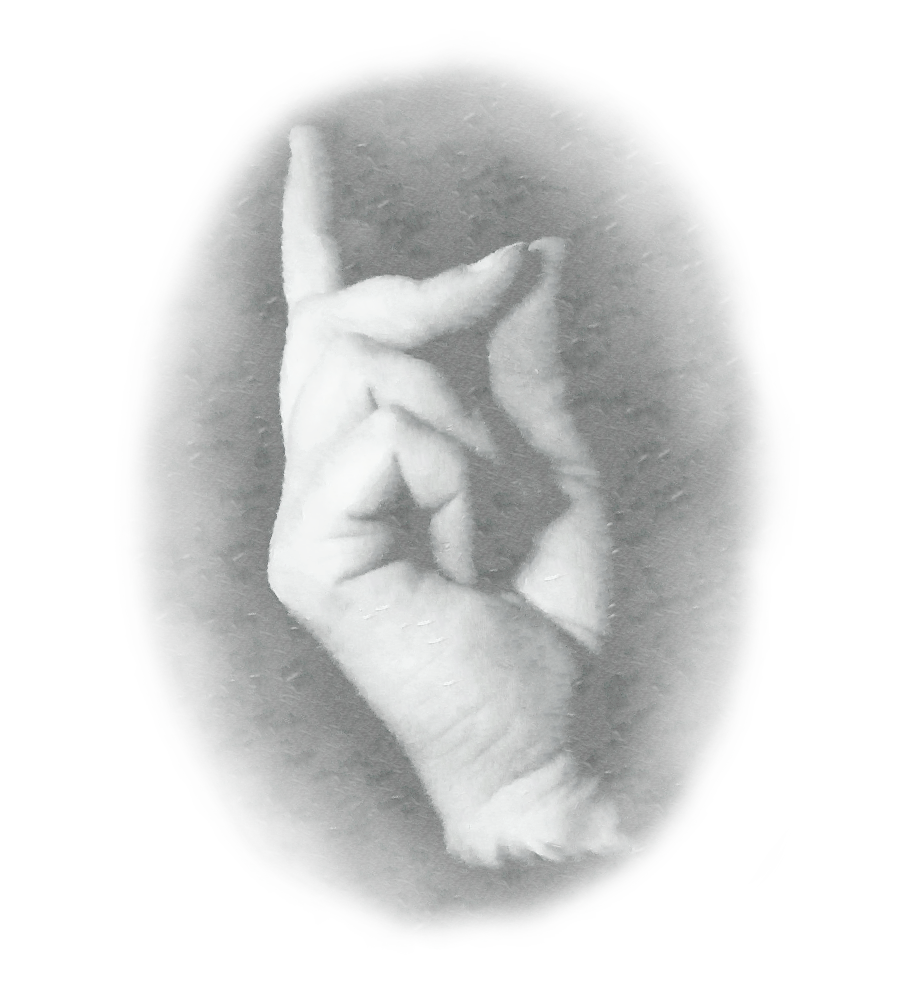
\includegraphics[scale=0.5]{bubble0.png} 
\end{vplace}

\vspace*{.5cm}
\LARGE\lumos{Eliezer\ \ \ Yudkowsky}
\normalsize


\vspace{2cm}
Find the original text at:\\
\url{http://hpmor.com} \\

\end{center}

% Begin subbook title

\cleartorecto
\begin{center}
\thispagestyle{empty}

\huge\lumos{Book\ \ }
\Huge\lumos{\hpBookNo} \vspace*{1cm}

\normalsize\lumos{\hpBookChar} \vspace*{0.2cm}

\footnotesize\lumos{and the}

\large\lumos{\hpBookTitle} \vspace*{0.5 cm}

\begin{vplace}
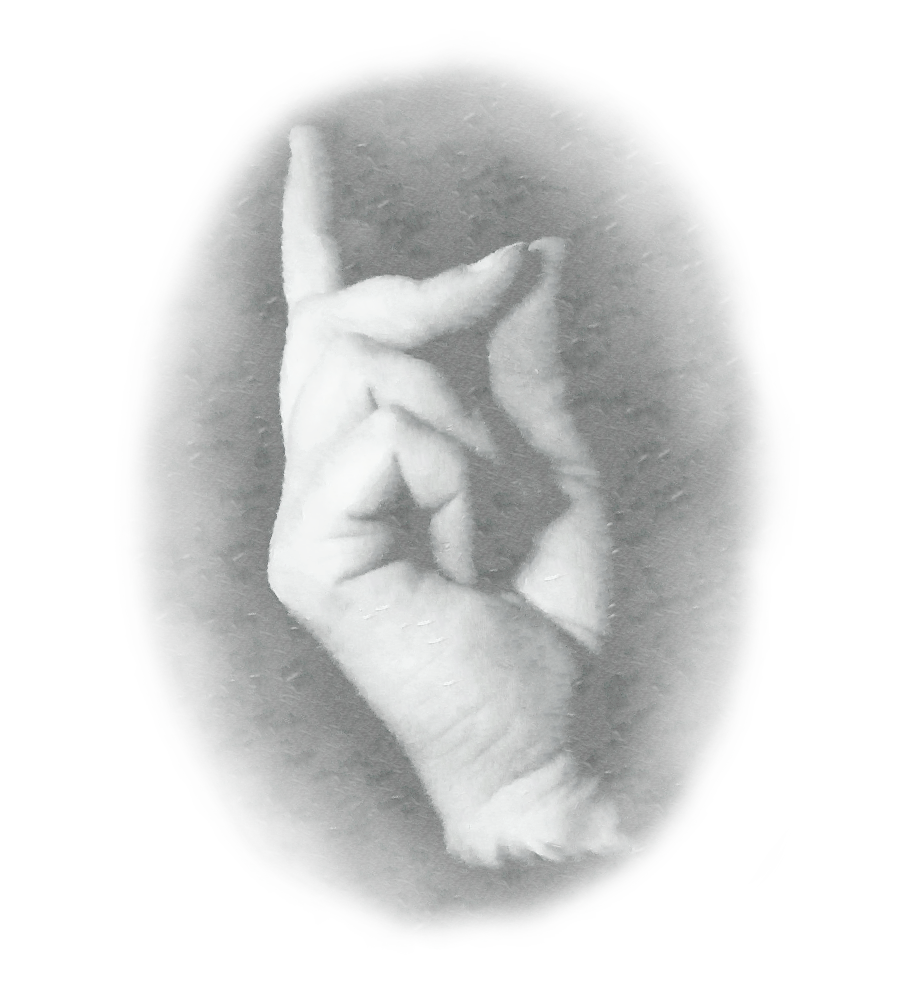
\includegraphics[scale=0.4]{bubble0.png} 
\end{vplace}

\vspace*{.5cm}
\LARGE\lumos{Eliezer\ \ \ Yudkowsky}
\normalsize

\vspace{2cm}
\mbox{\,}\\ \hpBookChapters

\end{center}

% End subbook title


\pagenumbering{gobble}
\cleartorecto
\renewcommand*{\hpmorchapbreak}{\ } % Prevent linebreaks in TOC
\renewcommand*{\printtoctitle}[1]{\centering\huge{\hp\MakeUppercase{#1}}}
\setlength{\cftbeforechapterskip}{.5\baselineskip plus 12pt minus 3pt}
\renewcommand*{\cftchapterleader}{\space—\space}
\renewcommand*{\cftchapterfillnum}[1]{%
 {\cftchapterleader}\nobreak%
 %\hbox to 1.5em{\cftchapterpagefont #1\hfil}%
 {#1}%
 \cftchapterafterpnum\par}
\setrmarg{0em}
\setlength\cftchapterindent{0pt}
\setlength\cftchapternumwidth{0pt}
\renewcommand*{\cftchapterafterpnum}{\cftparfillskip}
\renewcommand*{\cftchapterfont}{}%\small}

\renewcommand\chapternumberline[1]{\hfil\thispagestyle{empty}{\hp{\IfInteger{#1}{\NUMTONAME{#1}}{Appendix #1}}}\hfil\strut\par\nopagebreak\hfil}

\settocdepth{chapter}
\phantomsection
\label{contents}

\thispagestyle{empty}

\tableofcontents*

\clearpage
\thispagestyle{empty}
\hbox{}
\renewcommand*{\hpmorchapbreak}{\linebreak} % Restore previous functionality
\cleartoverso

% Headlines
\begin{Spacing}{0.95}
(International news headlines of April 7th, 1992:)
\vspace{1cm}

\emph{Toronto Magical Tribune:}

\headline{Entire British Wizengamot Reports Seeing\\
`Boy-Who-Lived' Frighten a Dementor}

\headline{Expert on Magical Creatures:\\
``Now You're Just Lying''}

\headline{France, Germany Accuse Britain\\
of Making the Whole Thing Up}

\emph{New Zealand Spellcrafter's Diurnal Notice:}

\headline{What Drove British Legislature Insane?\\
Could Our Government Be Next?}

\headline{Experts List Top 28 Reasons\\
To Believe It's Already Happened}

\emph{American Mage:}

\headline{Werewolf Clan to Become\\
First Inhabitants of Wyoming}

\emph{The Quibbler:}

\headline{Malfoy Flees Hogwarts\\
As Veela Powers Awaken}

\emph{Daily Prophet:}

\headline{Legal Tricks Free\\
``Mad Muggleborn''\\
As Potter Threatens Ministry\\
With Attack on Azkaban}
\end{Spacing}

% End headlines
\cleartorecto

}
\pagenumbering{arabic}
\setcounter{page}{1}

\chapter{Multiple Hypothesis Testing}

\subsection{Hypothesis: Voldemort\\
(April 8th, 1992, 7:22\PM)}

\lettrine{T}{he} four of them gathered once more around the ancient desk of the Headmaster
of Hogwarts, with its drawers within drawers within drawers, wherein all the
past paperwork of the Hogwarts School was stored; legend had it that
Headmistress Shehla had once gotten lost in that desk, and was, in fact, still
there, and wouldn't be let out again until she got her files organized. Minerva
didn't particularly look forward to inheriting those drawers, when she
inherited that desk someday—if any of them survived.

Albus Dumbledore was seated behind his desk, looking grave and composed.

Severus Snape was standing next to the dead Floo and its ashes, hovering
ominously like the vampire that students sometimes accused him of pretending to
be.

Mad-Eye Moody had been meant to join them, but was yet to arrive.

And Harry{\el}

A boy's small, thin frame, perched on the arm of his chair, as though the
energies running through him were too great to allow ordinary seating. Set
face, sweaty hair, intent green eyes, and within it all, the jagged
lightning-bolt of his never-healing scar. He seemed grimmer, now; even compared
to a single week earlier.

For a moment Minerva flashed back to her trip to Diagon Alley with Harry, what
seemed like ages and ages ago. There'd been this somber boy \emph{inside} that
Harry, somehow, even then. This wasn't entirely her own fault, or Albus's
fault. And yet there was something almost unbearably sad about the contrast
between the young boy she'd first met, and what magical Britain had made of
him. Harry had never had much of an ordinary childhood, she'd gathered; Harry's
adoptive parents had said to her that he'd spoken little and played less with
Muggle children. It was painful to think that Harry might have had only a few
months of playing beside the other children in Hogwarts, before the war's
demands had stripped it all away. Maybe there was another face that Harry
showed to the children his own age, when he wasn't staring down the Wizengamot.
But she couldn't stop herself from imagining Harry Potter's childhood as a heap
of firewood, and herself and Albus feeding the wooden branches, piece by piece,
into the flames.

"Prophecies are strange things," said Albus Dumbledore. The old wizard's eyes
were half-lidded, as though in weariness. "Vague, unclear, meaning escaping
like water held between loose fingers. Prophecy is ever a burden, for there are
no answers there, only questions."

Harry Potter was sitting tensely. "Headmaster Dumbledore," said the boy with
soft precision, "my friends are being targeted. Hermione Granger almost went to
Azkaban. The war has begun, as you put it. Professor Trelawney's prophecy is
key information for weighing up the balance of my hypotheses about what's going
on. Not to mention how silly it is—and \emph{dangerous}—that the Dark Lord
knows the prophecy and \emph{I don't}."

Albus looked a grim question at her, and she shook her head in reply; in
whatever unimaginable way Harry had discovered that Trelawney had made the
prophecy and that the Dark Lord knew of it, he hadn't learned that much from
her.

"Voldemort, seeking to avert that very prophecy, went to his defeat at your
hands," the old wizard said then. "His knowledge brought him only harm. Ponder
that carefully, Harry Potter."

"Yes, Headmaster, I do understand that. My home culture also has a literary
tradition of self-fulfilling and misinterpreted prophecies. I'll interpret with
caution, rest assured. But I've already guessed quite a bit. Is it safer for me
to work from partial guesses?"

Time passed.

"Minerva," said Albus. "If you would."

"The one{\el}" she began. The words came falteringly to her throat; she was
no actress. She couldn't imitate the deep, chilling tone of the original
prophecy; and yet somehow that tone seemed to carry all the \emph{meaning.}
"The one with the power to vanquish the Dark Lord approaches{\el} born to
those who have thrice defied him, born as the seventh month dies{\el}"

"\prophecy{And the Dark Lord shall mark him as his equal,}" came Severus's voice,
making her jump within her chair. The Potions Master loomed tall by the
fireplace. "\prophecy{But he shall have power the Dark Lord knows not{\el} and
either must destroy all but a remnant of the other, for those two different
spirits cannot exist in the same world.}"

That last line Severus spoke with so much foreboding that it chilled her bones;
it was almost like listening to Sybill Trelawney.

Harry was listening with a frown. "Can you repeat that?" said Harry.

"\prophecy{The one with the power to vanquish the Dark Lord approaches, born to
those who have thrice defied him, born as the seventh month}—"

"Actually, hold on, can you write that down? I need to analyze this
\emph{carefully}—"

This was done, with both Albus and Severus watching the parchment hawklike, as
though to make sure that no unseen hand reached in and snatched the precious
information away.

"Let's see{\el}" Harry said. "I'm male and born on July 31st, check. I did
in fact vanquish the Dark Lord, check. Ambiguous pronoun in line two{\el}
but I wasn't born yet so it's hard to see how my parents could have thrice
defied \emph{me.} This scar is an obvious candidate for the mark{\el}" Harry
touched his forehead. "Then there's the power the Dark Lord knows not, which
probably refers to my scientific background—"

"No," said Severus.

Harry looked at the Potions Master in surprise.

Severus's eyes were closed, his face tightened in concentration. "The Dark Lord
could obtain that power by studying the same books as you, Potter. But the
prophecy did not say, \emph{power the Dark Lord has not.} Nor even, \emph{power
the Dark Lord cannot have.} She spoke of \emph{power the Dark Lord knows
not}{\el} it will be something stranger to him than Muggle artifacts.
Something perhaps that he cannot comprehend at all, even having seen it{\el}"

"Science is not a bag of technological tricks," Harry said. "It's not just the
Muggle version of a wand. It's not even knowledge like memorizing the periodic
table. It's a different way of \emph{thinking.}"

"Perhaps{\el}" the Potions Master murmured, but his voice was skeptical.

"It is hazardous," Albus said, "to read too far into a prophecy, even if you
have heard it yourself. They are things of exceeding frustration."

"So I see," Harry said. His hand rose up, rubbed the scar on his forehead.
"But{\el} okay, if \emph{this} is really all we know{\el} look, I'll just
put it bluntly. How do you \emph{know} that the Dark Lord actually survived?"

"\emph{What?}" she cried. Albus just sighed and leaned back in the vast
Headmaster's chair.

"Well," Harry said, "imagine how this prophecy sounded back when it was made.
You-Know-Who learns the prophecy, and it sounds like I'm destined to grow up
and overthrow him. That the two of us are meant to have a final battle where
either of us must destroy all but a remnant of the other. So You-Know-Who
attacks Godric's Hollow and \emph{immediately} gets vanquished, leaving behind
\emph{some} remnant which may or may not be his disembodied soul. Maybe the
Death Eaters are his remnant, or the Dark Mark. This prophecy could already be
fulfilled, is what I'm saying. Don't get me wrong—I do realize that my
interpretation sounds stretched. Trelawney's phrasing doesn't seem natural for
describing \emph{only} the events that historically happened on October 31st,
1981. Attacking a baby and having the spell bounce off, isn't something you'd
normally call `the power to vanquish'. But if you think of the prophecy as
being about \emph{several} possible futures, only \emph{one} of which was
actually realized on Halloween, then the prophecy could already be complete."

"But—" Minerva blurted. "But the raid on Azkaban—"

"\emph{If} the Dark Lord survived, then sure, he's the most likely suspect for
the Azkaban breakout," Harry said reasonably. "You could even say that the
Azkaban breakout is Bayesian evidence for the Dark Lord surviving, because an
Azkaban breakout is more likely to happen in worlds where he's alive than
worlds where he's dead. But it's not \emph{strong} Bayesian evidence. It's not
something that \emph{can't possibly happen} unless the Dark Lord is alive.
Professor Quirrell, who \emph{didn't} start from the assumption that
You-Know-Who was still around, had no trouble thinking of his own explanation.
To him, it was obvious that some powerful wizard might want Bellatrix Black
because she knew a secret of the Dark Lord's, like some of his magical
knowledge that he'd told to only her. The priors against anyone surviving their
body's death are very low, even if it's magically possible. \emph{Most} times
it doesn't happen. So if it's \emph{just} the Azkaban breakout{\el} I'd have
to say formally that it isn't enough Bayesian evidence. The improbability of
the evidence assuming that the hypothesis is false, is not commensurate with
the prior improbability of the hypothesis."

"No," Severus said flatly. "The prophecy is not yet fulfilled. I would know if
it were."

"Are you \emph{sure} of that?"

"Yes, Potter. If the prophecy had already come true, I would \emph{understand}
it! I heard Trelawney's words, I remember Trelawney's voice, and if I knew the
events that matched the prophecy, I would \emph{recognize} them. What has
already happened{\el} does \emph{not} fit." The Potions Master spoke with
certainty.

"I'm not really sure what to do with that statement," Harry said. His hand rose
up, absently rubbed at his forehead. "Maybe it's just what you \emph{think}
happened that doesn't fit, and the true history is different{\el}"

"Voldemort \emph{is} alive," Albus said. "There are other indications."

"Such as?" Harry's reply was instant.

Albus paused. "There are terrible rituals by which wizards have returned from
death," Albus said slowly. "That much, anyone can discern within history and
legend. And yet those books are missing, I could not find them; it was
Voldemort who removed them, I am sure—"

"So you \emph{can't} find any books on immortality, and that proves that
You-Know-Who has them?"

"Indeed," said Albus. "There is a certain book—I will not name it
aloud—missing from the Restricted Section of the Hogwarts library. An ancient
scroll which should have been at Borgin and Burkes, with only an empty place on
a shelf to show where it was—" The old wizard stopped. "But I suppose," the
old wizard said, as though to himself, "you will say that even if Voldemort
tried to make himself immortal, it does not prove that he succeeded{\el}"

Harry sighed. "Proof, Headmaster? There are only ever probabilities. If there
are known, particular books on immortality rituals which are missing, that
increases the probability that someone attempted one. Which, in turn, raises
the prior probability of the Dark Lord surviving his death. This I concede, and
thank you for contributing the fact. The question is whether the prior
probability goes up \emph{enough.}"

"Surely," Albus said quietly, "if you concede even a \emph{chance} that
Voldemort survived, that is worth guarding against?"

Harry inclined his head. "As you say, Headmaster. Though once a probability
drops low enough, it's also an error to go on obsessing about it{\el} Given
that books on immortality are missing, and that this prophecy would sound
\emph{somewhat} more natural if it refers to the Dark Lord and I having a
future battle, I agree that the Dark Lord being alive is a probability, not
just possibility. But other probabilities must \emph{also} be taken into
account—and in the probable worlds where You-Know-Who is \emph{not} alive,
someone else framed Hermione."

"Foolishness," Severus said softly. "Utter foolishness. The Dark Mark has not
faded, nor has its master."

"See, \emph{that's} what I mean by formally insufficient Bayesian evidence.
Sure, it sounds all grim and foreboding and stuff, but is it \emph{that}
unlikely for a magical mark to stay around after the maker dies? Suppose the
mark is certain to continue while the Dark Lord's sentience lives on, but
\emph{a priori} we'd only have guessed a twenty percent chance of the Dark Mark
continuing to exist after the Dark Lord dies. Then the observation, `The Dark
Mark has not faded' is five times as likely to occur in worlds where the Dark
Lord is alive as in worlds where the Dark Lord is dead. Is that really
commensurate with the prior improbability of immortality? Let's say the prior
odds were a hundred-to-one against the Dark Lord surviving. If a hypothesis is
a hundred times as likely to be false versus true, and then you see evidence
five times more likely if the hypothesis is true versus false, you should
update to believing the hypothesis is twenty times as likely to be false as
true. Odds of a hundred to one, times a likelihood ratio of one to five, equals
odds of twenty to one that the Dark Lord is dead—"

"\emph{Where} are you getting all these numbers, Potter?"

"That \emph{is} the admitted weakness of the method," Harry said readily. "But
what I'm \emph{qualitatively} getting at is why the observation, `The Dark Mark
has not faded', is not adequate support for the hypothesis, `The Dark Lord is
immortal.' The evidence isn't as extraordinary as the claim." Harry paused.
"Not to mention that even if the Dark Lord is alive, he doesn't \emph{have} to
be the one who framed Hermione. As a cunning man once said, there could be more
than one plotter and more than one plan."

"Such as the Defense Professor," Severus said with a thin smile. "I suppose I
must agree that he is a suspect. It was the Defense Professor last year, after
all; and the year before that, and the year before \emph{that}."

Harry's eyes dropped back to the parchment in his lap. "Let's move on. Are
we \emph{certain} that this Prophecy is accurate? Nobody messed with Professor
McGonagall's memory, maybe edited or subtracted a line?"

Albus paused, then spoke slowly. "There is a great spell laid over Britain,
recording every prophecy said within our borders. Far beneath the Most Ancient
Hall of the Wizengamot, in the Department of Mysteries, they are recorded."

"The Hall of Prophecy," Minerva whispered. She'd read about that place, said to
be a great room of shelves filled with glowing orbs, one after another
appearing over the years. Merlin himself had wrought it, it was said; the
greatest wizard's final slap to the face of Fate. Not all prophecies conduced
to the good; and Merlin had wished for at least those spoken of in prophecy, to
know what had been spoken \emph{of} them. That was the respect Merlin had given
to their free will, that Destiny might not control them from the outside,
unwitting. Those mentioned within a prophecy would have an glowing orb float to
their hand, and then hear the prophet's true voice speaking. Others who tried
to touch an orb, it was said, would be driven mad—or possibly just have their
heads explode, the legends were unclear on this point. Whatever Merlin's
original intention, the Unspeakables hadn't let anyone enter in centuries, so
far as she'd heard. \emph{Works of the Ancient Wizards} had stated that later
Unspeakables had discovered that tipping off the subjects of prophecies could
interfere with seers releasing whatever temporal pressures they released; and
so the heirs of Merlin had sealed his Hall. It did occur to Minerva to wonder
(now that she'd spent a few months around Mr.~Potter) how anyone could possibly
\emph{know} that; but she also knew better than to ask Albus, in case Albus
tried to tell her. Minerva firmly believed that you only ought to worry about
Time if you were a clock.

"The Hall of Prophecy," Albus confirmed lowly. "Those who are spoken of in a
prophecy, may listen to that prophecy there. Do you see the implication, Harry?"

Harry frowned. "Well, I could listen to it, or the Dark Lord{\el} oh, my
\emph{parents}. Those who had thrice defied him. They were also mentioned in
the prophecy, so they could hear the recording?"

"If James and Lily heard anything different from what Minerva reported," Albus
said evenly, "they did not say so to me."

"You took James and Lily \emph{there?}" Minerva said.

"Fawkes can go to many places," Albus said. "Do not mention the fact."

Harry was staring directly at Albus. "Can \emph{I} go to this Department of
Mysteries place and hear the recorded prophecy? The original tone of voice
might be helpful, from what I've heard."

Light glinted from the reflection of Albus's half-moon glasses as the old
wizard slowly shook his head. "I think that would be unwise," Albus said. "For
reasons beyond the obvious. It is dangerous, that place which Merlin made; more
dangerous to some people than others."

"I see," Harry said tonelessly, and looked back down at the parchment. "I'll
take the prophecy as assumed accurate for now. The next part says that the Dark
Lord has marked me as his equal. Any ideas on what that means exactly?"

"Surely not," said Albus, "that you must imitate his ways, in any wise."

"I'm not \emph{dumb,} Headmaster. Muggles have worked out a thing or two about
temporal paradoxes, even if it's all theoretical to them. I won't throw away my
ethics just because a signal from the future claims it's going to happen,
because then that becomes the only reason why it happened in the first place.
Still, what \emph{does} it mean?"

"I do not know," said Severus.

"Nor I," she said.

Harry took out his wand, turned it over in his hands, gazing meditatively at
the wood. "Eleven inches, holly, with a core of phoenix feather," Harry said.
"And the phoenix whose tail feather is in this wand, only ever gave one other,
which Mr{\el} what was his name, Olive-something{\el} made into the core
of the Dark Lord's wand. \emph{And} I'm a Parselmouth. It seemed like a lot of
coincidence even then. And now I find out there's a prophecy stating that I'll
be the Dark Lord's equal."

Severus's eyes were thoughtful; the Headmaster's gaze, unreadable.

"Could it be," Minerva said falteringly, "that You-Know-Who—that
Voldemort—transferred some of his own powers to Mr.~Potter, the night he gave
him that scar? Not something he intended to do, surely. Still{\el} I don't
see how Mr.~Potter could be his \emph{equal,} if he had any less magic than the
Dark Lord himself{\el}"

"Meh," said Harry, still looking meditatively at his wand. "I'd fight the Dark
Lord without any magic at all, if I had to. \emph{Homo sapiens} didn't become
the dominant species on this planet by having the sharpest claws or hardest
armor—though I suppose some of that point may be lost on wizards. Still, it's
beneath my dignity as a human being to be scared of anything that isn't smarter
than I am; and from what I've heard, on that particular dimension the Dark Lord
wasn't very scary."

The Potions Master spoke, his voice taking on some of his customary
contemptuous drawl. "You imagine yourself more intelligent than the Dark Lord,
Potter?"

"Yes, in fact," said Harry, pulling back the left sleeve of his robes, and
rolling up the shirtsleeve beneath to expose the bare elbow. "Oh, that reminds
me! Let's make sure nobody here has the clearly visible tattoo in the standard,
easily checkable location which would mark them as a secret enemy spy."

Albus made a quieting gesture that halted the Potions Master before he could
say anything scathing. "Tell me, Harry," Albus said, "how would \emph{you} have
crafted the Dark Mark?"

"Nonstandard locations," Harry said promptly, "not easily found without
embarrassment and fuss, though of course any security-conscious person would
check anyway. Make it smaller, if possible. Overlay another non-magical tattoo
to obscure the exact shape—better yet, cover it with a layer of fake skin—"

"Cunning indeed," Albus said. "But tell me, suppose you could craft any
conditions you wished into the Mark, fading it or raising it as you wished.
What would you do then?"

"Make it completely invisible at all times," Harry said in tones of stating the
obvious. "You don't want there to be any detectable difference between a spy
and a non-spy."

"Suppose you are more cunning still," Albus said. "You are a master of
trickery, a master of deception, and you employ your abilities to the fullest."

"Well—" The boy stopped, frowning. "It seems unnecessarily complicated, more
like a tactic a villain would use in a role-playing game than something you'd
try in a real-life war. But I suppose you could put fake Dark Marks on people
who aren't really Death Eaters, and keep the Dark Marks on the real Death
Eaters invisible. But then there's the question of why people would start
believing in the first place that the Dark Mark identified a Death
Eater{\el} I'd have to think about it for at least five minutes, if I were
going to take the problem seriously."

"I ask you this," Albus said, still in that mild tone, "because I did indeed,
in the early days of the war, perform such tests as you suggested. The Order
survived my folly only because Alastor did not trust in the bare arms we saw. I
had thought, afterward, that the bearers of the Mark might hide it or show it
at their will. And yet when we hied Igor Karkaroff before the Wizengamot, that
Mark showed clear on his arm, for all that Karkaroff wished to protest his
innocence. What true rule may govern the Dark Mark, I do not know. Even Severus
is still bound by his Mark not to reveal its secrets to any who do not know
them."

"Oh, well \emph{that} makes it \emph{obvious}," Harry said promptly. "Wait,
hold on—you were a \emph{Death Eater?}" Harry transferred his stare to
Severus.

Severus returned a thin smile. "I still am, so far as they know."

"Harry," said Albus, eyes only for the boy. "What do you mean, that makes it
obvious?"

"Information theory 101," the boy said in a lecturing tone. "Observing variable
X conveys information about variable Y, if and only if the possible values of X
have different probabilities given different states of Y. The instant you hear
about anything whatsoever that varies between a spy and a nonspy, you should
immediately think of exploiting it to distinguish spies from nonspies.
Similarly, to distinguish reality from lies, you need a process which behaves
differently in the presence of truth and falsehood—that's why `faith' doesn't
work as a discriminant, while `make experimental predictions and test them'
does. You say someone with the Dark Mark can't reveal its secrets to anyone who
doesn't already know them. So to find out how the Dark Mark operates, write
down every way you can imagine the Dark Mark \emph{might} work, then watch
Professor Snape try to tell each of those things to a confederate—maybe one
who doesn't know what the experiment is about—I'll explain binary search
later so that you can play Twenty Questions to narrow things down—and
whatever he \emph{can't} say out loud is true. His silence would be something
that behaves differently in the presence of true statements about the Mark,
versus false statements, you see."

Minerva's mouth was hanging open, she realized; and she closed it abruptly.
Even Albus looked surprised.

"And after that, like I said, \emph{any} behavioral difference between spies
and nonspies can be used to identify spies. Once you've identified at least one
magically censored secret of the Dark Mark, you can test someone for the Dark
Mark by seeing if they can reveal that secret to somebody who doesn't already
know it—"

"\emph{Thank you, Mr.~Potter.}"

Everyone looked at Severus. The Potions Master was straightening, his teeth
bared in a grimace of angry triumph. "Headmaster, I can now speak freely of the
Mark. If we know we are caught for a Death Eater, before others who have not
yet seen our bare arms, our Mark reveals itself whether we will it or no. But
if they have already seen our arms bare, it does not reveal itself; nor if we
are only being tested from suspicion. Thus the Dark Mark seems to identify
Death Eaters—but only those already found, you perceive."

"Ah{\el}" Albus said. "Thank you, Severus." He closed his eyes briefly.
"That would indeed explain why Black escaped even Peter's notice{\el} ah,
well. And Harry's proposed test?"

The Potions Master shook his head. "The Dark Lord was no fool, despite Potter's
delusions. The moment such a test is suspected, the Mark ceases to bind our
tongues. Yet I could not hint at the possibility, but only wait for another to
deduce it." Another thin smile. "I would award you a good many House points,
Mr.~Potter, if it would not compromise my cover. But as you can see, the Dark
Lord was quite cunning." His gaze grew more distant. "Oh," Severus breathed,
"he was \emph{very} cunning indeed{\el}"

Harry Potter sat still for a long moment.

Then—

"No," Harry said. The boy shook his head. "No, that can't \emph{actually} be
true. First of all, we're talking about the kind of logic puzzle that would
appear in chapter \emph{one} of a Raymond Smullyan book, nowhere \emph{near}
the level of what Muggle scientists do for a living. And second, for all I
know, it took the Dark Lord five months of thinking to invent the puzzle I just
solved in five seconds—"

"Is it \emph{that} inconceivable to you, Potter, that anyone could be so
intelligent as yourself?" The Potions Master's voice held more curiosity than
scorn.

"It's called a base rate, Professor Snape. The evidence is equally compatible
with the Dark Lord inventing that puzzle over the course of five months or over
the course of five seconds, but in any given population there'll be many more
people who can do it in five months than in five seconds{\el}" Harry pasted
a hand against his forehead. "Darn it, how can I explain this? I suppose, from
your perspective, the Dark Lord came up with a clever puzzle and I cleverly
solved it and that makes us look \emph{equal}."

"I remember your first day of Potions class," the Potions Master said dryly. "I
think you have a ways still to go."

"Peace, Severus," Albus said. "Harry has already accomplished more than you
know. Yet tell me, Harry—why \emph{do} you believe the Dark Lord is less than
you? Surely he is a damaged soul in many ways. But cunning for cunning—you
are not yet ready to face him, I would judge; and I know the full tally of your
deeds."
\sbreak
The frustrating thing about this conversation was that Harry \emph{couldn't say
his actual reasons for disagreeing,} which violated several basic principles of
cooperative discourse.

He couldn't explain how Bellatrix had really been removed from Azkaban—not by
You-Know-Who in any guise, but by the combined wits of Harry and Professor
Quirrell.

Harry didn't want to say in front of Professor McGonagall that the existence of
brain damage implied that there were no such things as souls. Which made a
successful immortality ritual{\el} well, not \emph{impossible,} Harry
certainly intended to forge a road to magical immortality \emph{someday}, but
it would be a \emph{lot harder} and require \emph{much more ingenuity} than
just binding an already-existent soul to a lich's phylactery. Which no
intelligent wizard would bother doing in the first place, if they knew their
souls were immortal.

And the true and honest reason Harry knew the Dark Lord couldn't have been
\emph{that} smart{\el} well{\el} there wasn't any tactful way to say it,
but{\el}

Harry had \emph{been} to a convocation of the Wizengamot. He'd \emph{seen} the
laughable `security precautions', if you could call them that, guarding the
deepest levels of the Ministry of Magic. They didn't even have the Thief's
Downfall which goblins used to wash away Polyjuice and Imperius Curses on
people entering Gringotts. The obvious takeover route would be to Imperius the
Minister of Magic and a few department heads, and owl a hand grenade to anyone
too powerful to Imperius. Or owl them knockout gas, if you needed them alive
and in a state of Living Death to take hairs for Polyjuice potions.
Legilimency, False Memories, the Confundus Charm—it was ridiculous, the
magical world was \emph{supersaturated} with ways to cheat. Harry might not do
any of those things himself, during his own takeover of Britain, since he was
constrained by Ethics{\el} well, Harry \emph{might} do some of the lesser
ones, since Polyjuice or a temporary Confundus or read-only Legilimency all
sounded better than an extra day of Azkaban{\el} but{\el}

If Harry hadn't been constrained by Ethics, it was possible he could've wiped
out the eviller sections of the Wizengamot that day; all by himself, using only
a first-year's magical power, on account of being clever enough to figure out
Dementors. Though Harry might not have been in such a great political position
after that, the surviving Wizengamot members might've found it easy and cheap
to disavow his actions for P.R. purposes and condemn him, even if the smarter
ones realized it was for the greater good{\el} but \emph{still.}

If you were completely unrestrained by ethics, armed with the ancient secrets
of Salazar Slytherin, had dozens of powerful followers including Lucius Malfoy,
and it took you more than ten years to \emph{fail} to overthrow the government
of magical Britain, it meant you were stupid.

"How can I put this{\el}" Harry said. "Look, Headmaster, you've got ethics,
there's a lot of battle tactics you don't use because you're not evil. And you
fought the Dark Lord, a tremendously powerful wizard who wasn't so restrained,
and you held him off \emph{anyway}. If You-Know-Who had been super-smart
\emph{on top of that}, you'd be \emph{dead. All} of you. You'd have died
\emph{instantly}—"

"Harry," Professor McGonagall said. Her voice was faltering. "Harry, we almost
\emph{did} all die. More than half the Order of the Phoenix died. If not for
Albus—Albus Dumbledore, the greatest wizard in two centuries, Harry—we
surely would have perished."

Harry passed a hand across his forehead. "I'm sorry," Harry said. "I'm not
trying to minimize what you went through. I know that You-Know-Who was a
completely evil, incredibly powerful Dark Wizard with dozens of powerful
followers, and that's{\el} bad, yes, definitely bad. It's just{\el}"
\emph{All that isn't on remotely the same threat scale as the enemy being
smart, in which case they Transfigure botulinum toxin and sneak a millionth of
a gram into your teacup.} Was there any safe way to convey that concept without
citing specifics? Harry couldn't think of one.

"Please, Harry," said Professor McGonagall. "Please, Harry, I beg
you—\emph{take the Dark Lord seriously!} He is more dangerous than—" The
senior witch seemed to be having trouble finding words. "He is \emph{far} more
dangerous than Transfiguration."

Harry's eyebrows went up before he could stop himself. A dark chuckle came from
Severus Snape's direction.

\emph{Um,} said the voice of Ravenclaw within him. \emph{Um, honestly Professor
McGonagall is right, we're not taking this as seriously as we'd take a
scientific problem. The difficult thing is to react} at all \emph{to new
information, instead of just flushing it out the window. Right now it looks
like we didn't shift belief} at all \emph{after encountering an unexpected,
important argument. Our dismissal of Lord Voldemort as a serious threat}
was \emph{originally based on the Dark Mark being blatantly stupid. It would
require a focused effort to de-update and suspect the whole garden-path of
reasoning we went down based on that false assumption, and we're} not \emph{
putting in that effort right now.}

"All right," Harry said, just as Professor McGonagall seemed to be about to
speak again. "All right, to take this seriously, I need to stop and think for
five minutes."

"Please do," said Albus Dumbledore.

Harry closed his eyes.

His Ravenclaw side divided into three.

\emph{Probability estimate,} said Ravenclaw One, who was acting as moderator.
\emph{That the Dark Lord is alive, and as smart as we are, and hence a genuine
threat.}

\emph{Why aren't all his enemies already dead?} said Ravenclaw Two, who was
prosecuting.

\emph{Note,} said Ravenclaw One, \emph{we had already thought of that argument
so we can't use it to shift belief} again \emph{each time we rehearse it.}

\emph{But what's the actual flaw in the logic?} said Ravenclaw Two. \emph{In
worlds with a smart Lord Voldemort, everyone in the Order of the Phoenix died
in the first five minutes of the war. The world doesn't look like that, so we
don't live in that world. QED.}

\emph{Is that really certain?} asked Ravenclaw Three, who'd been appointed as
the defender. \emph{Maybe there was some reason Lord Voldemort} wasn't
\emph{fighting all-out back then—}

\emph{Like what?} demanded Ravenclaw Two. \emph{Furthermore, whatever your
excuse, I demand that the probability of your hypothesis be penalized in
accordance with its added complexity—}

\emph{Let Three talk,} said Ravenclaw One.

\emph{Okay{\el} look,} said Ravenclaw Three. \emph{First of all, we don't}
know \emph{that anyone can take over the Ministry just with mind control. Maybe
magical Britain is really an oligarchy and you need enough military power to
intimidate the family heads into submission—}

\emph{Imperius them too,} interjected Ravenclaw Two.

\emph{—and the oligarchs have Thief's Downfall in the entrances to}
their \emph{homes—}

\emph{Complexity penalty!} cried Ravenclaw Two. \emph{More epicycles!}

—\emph{oh, be reasonable,} said Ravenclaw Three. \emph{We haven't actually}
seen \emph{anyone taking over the Ministry with a couple of well-placed
Imperius curses. We don't} know \emph{that it can actually be done that easily.}

\emph{But,} said Ravenclaw Two, \emph{even taking that into account{\el} it
really seems like there should've been} some \emph{other way. Ten years of
failure, really? Using only conventional terrorist tactics? That's just{\el}
not even} trying.

\emph{Maybe Lord Voldemort did have more creative ideas,} replied Ravenclaw
Three, \emph{but he didn't want to tip his hand to} other \emph{countries'
governments, didn't want} them \emph{to know how vulnerable they were and
install Thief's Downfall in} their \emph{Ministries. Not until he had Britain
as a base and enough servants to subvert} all \emph{the other major governments
simultaneously.}

\emph{You're assuming he wants to conquer the whole world,} noted Ravenclaw Two.

\emph{Trelawney prophesized that he would be our equal,} intoned Ravenclaw
Three solemnly. \emph{Therefore, he wanted to take over the world.}

\emph{And if he is your equal, and you do have to fight him—}

For an instant, Harry's mind tried to imagine the specter of two
\emph{creative} wizards fighting an all-out-war against each other.

Harry had noted all the Charms and Potions in his first-year books that could
be creatively used to kill people. He hadn't been able to help himself.
Literally. He'd \emph{tried} to stop his brain from doing it each time, but it
was like looking at a fish and trying to stop your brain from noticing it was a
fish. What someone could creatively do with seventh-year, or Auror-level, or
ancient lost magic such as Lord Voldemort had possessed{\el} didn't bear
thinking about. A magically-superpowered creative-genius psychopath wasn't a
`threat', it was an extinction event.

Then Harry shook his head, dismissing the gloomy line his reasoning had been
going down. The question was whether there was a significant probability of
facing anything so terrible as a Dark Rationalist in the first place.

\emph{Prior odds that someone attempting an immortality ritual would actually
have it work{\el}}

Call it one to a thousand, at a generous overestimate; it was not the case that
roughly one wizard in a thousand survived their death. Though, admittedly Harry
didn't have data on how many had attempted immortality rituals first.

\emph{What if the Dark Lord} is \emph{as smart as us?} said Ravenclaw Three.
\emph{You know, the way Trelawney prophesied him being our} equal. \emph{Then
he would} make \emph{his immortality ritual work. P.S., don't forget that
`destroy all but a remnant of the other' line.}

Requiring that level of intelligence was an additional burdensome detail; prior
odds of a random population member being that intelligent were low{\el}

But Lord Voldemort wasn't a randomly selected wizard, he was one particular
wizard in the population who'd come to everyone's attention. The puzzle of the
Mark implied a certain minimum level of intelligence, even if (hypothetically)
the Dark Lord had taken longer to think it through. Then again, in the Muggle
world, all of the extremely intelligent people Harry knew about from history
had \emph{not} become evil dictators or terrorists. The closest thing to that
in the Muggle world was hedge-fund managers, and none of \emph{them} had tried
to take over so much as a third-world country, a point which put upper bounds
on both their possible evil and possible goodness.

There were hypotheses where the Dark Lord was smart and the Order of the
Phoenix \emph{didn't} just instantly die, but those hypotheses were more
complicated and ought to get complexity penalties. After the complexity
penalties of the further excuses were factored in, there would be a large
likelihood ratio from the hypotheses `The Dark Lord is smart' versus `The Dark
Lord was stupid' to the observation, `The Dark Lord did not instantly win the
war'. That was probably worth a 10:1 likelihood ratio in favor of the Dark Lord
being stupid{\el} but maybe not 100:1. You couldn't actually say that `The
Dark Lord instantly wins' had a probability of \emph{more} than 99 percent,
assuming the Dark Lord started out smart; the sum over all possible excuses
would be more than .01.

And then there was the Prophecy{\el} which might or might not have
\emph{originally} included a line about how Lord Voldemort would
\emph{immediately} die if he confronted the Potters. Which Albus Dumbledore had
then edited in Professor McGonagall's memory, in order to lure Lord Voldemort
to his doom. If there \emph{was} no such line, the Prophecy did sound
\emph{somewhat} more like You-Know-Who and the Boy-Who-Lived were destined to
have some later confrontation. But in \emph{that} case, it was less likely that
Dumbledore would've come up with a plausible-sounding excuse not to take Harry
to the Hall of Prophecy{\el}

Harry was wondering if he could even \emph{get} a Bayesian calculation out of
this. Of course, the point of a subjective Bayesian calculation wasn't that,
after you made up a bunch of numbers, multiplying them out would give you an
exactly right answer. The real point was that the \emph{process} of making up
numbers would force you to tally all the relevant facts and weigh all the
relative probabilities. Like realizing, as soon as you actually \emph{thought}
about the probability of the Dark Mark not-fading \emph{if} You-Know-Who
\emph{was} dead, that the probability wasn't low enough for the observation to
count as strong evidence. One version of the process was to tally hypotheses
and list out evidence, make up all the numbers, do the calculation, and then
throw out the final answer and go with your brain's gut feeling \emph{after}
you'd forced it to really \emph{weigh} everything. The trouble was that the
items of evidence weren't conditionally independent, and there were multiple
interacting background facts of interest{\el}

{\el} well, \emph{one} thing at least was certain.

If the calculation could be done at all, it was going to take a piece of paper
and a pencil.

In the fireplace at one side of the Headmaster's office, the flames suddenly
flared up, turning from orange to bright billious green.

"Ah!" said Professor McGonagall into the uncomfortable non-silence. "That would
be Mad-Eye Moody, I suppose."

"Let this matter bide for now," the Headmaster said in some relief, as he too
turned to regard the Floo. "I believe we are about to receive some news
regarding it, as well."
\sbreak
\vspace{-2\baselineskip}
\subsection{Hypothesis: Hermione Granger\\
(April 8th, 1992, 6:53\PM)}

Meanwhile in the Great Hall of Hogwarts, as the students who didn't have secret
meetings with the Headmaster bustled about their dinner around four huge
tables—

"It's funny," Dean Thomas said thoughtfully. "I didn't believe the General when
he said that what we learned would change us forever, and we'd never be able to
return to a normal life afterward. Once we knew. Once we saw what \emph{he}
could see."

"I know!" said Seamus Finnigan. "I thought it was just a joke too! Like, you
know, everything else General Chaos ever said ever."

"But now—" Dean said sadly. "We \emph{can't} go back, can we? It'd be like
going back to a Muggle school after having been to Hogwarts. We've just{\el}
we've just got to stay around each other. That's all we can do, or we'll go
crazy."

Seamus Finnigan, next to him, just nodded wordlessly and ate another bite of
veldbeest.

Around them, the conversation at the Gryffindor table continued. It wasn't as
\emph{relentless} as it'd been yesterday, but now and then the topic wandered
back.

"Well, there must've been \emph{some} sort of love triangle," said a
second-year witch named Samantha Crowley (she never answered when asked if
there was any relation). "The question is, which ways was it \emph{going}
before it all went wrong? Who was in love with who—and whether or not that
person loved them back—I don't know \emph{how} many possibilities there
are—"

"Sixty-four," said Sarah Varyabil, a blossoming beauty who probably should've
been Sorted into Ravenclaw or Hufflepuff instead. "No, wait, that's wrong. I
mean, if nobody loved Malfoy and Malfoy didn't love anyone then he wouldn't
really be part of the love triangle{\el} this is going to take Arithmancy,
could you all wait two minutes?"

"\emph{I,} for one, think it perfectly clear that Granger is Potter's moirail,
and that Potter was auspisticing between Malfoy and Granger." The witch who'd
spoken nodded with the self-satisfaction of someone who has just precisely
nailed down a complicated issue.

"Those aren't even words," objected a young wizard. "You're just making them up
as you go."

"Sometimes you can't describe a thing using \emph{real} words."

"It's so \emph{sad,}" said Sherice Ngaserin, who actually had tears in her
eyes. "They were just—they were just so \emph{obviously} meant to be
together!"

"You mean Potter and Malfoy?" said a second-year named Colleen Johnson. "I
know—their families hated each other so much, there's no way they
\emph{couldn't} fall in love—"

"No, I mean all three of them," said Sherice.

This produced a brief pause in the huddled conversation. Dean Thomas was
quietly choking on his lemonade, trying not to make any sounds as it trickled
out of his mouth and soaked into his shirt.

"\emph{Wow,}" said a dark-haired witch by the name of Nancy Hua. "That's
really{\el} \emph{sophisticated} of you, Sherice."

"Look, you all, we need to keep this realistic," said Eloise Rosen, a tall
witch who'd been General of an army and hence spoke with an air of authority.
"We \emph{know}—because she kissed him—that Granger was in love with
Potter. So the only reason she'd try to kill Malfoy is if she knew that she was
losing Potter to him. There's no need to make it all sound so
complicated—you're all acting like this is a play instead of real life!"

"But even if Granger was in love, it's still funny that she'd just \emph{snap}
like that," said Chloe, whose black robes combined with her night-black skin to
make her look like a darkened silhouette. "I don't know{\el} I think maybe
there's more to this than just a romance novel gone wrong. I think maybe most
people haven't got any idea at all what's going on."

"\emph{Yes! Thank you!}" burst out Dean Thomas. "Look—don't you
realize—like Harry Potter \emph{told} us all—if you didn't \emph{predict}
that something would happen, if it took you completely by surprise, then what
you believed about the world when you \emph{didn't} see it coming, isn't enough
to explain{\el}" Dean's voice trailed off, as he saw that nobody was
listening. "It's \emph{completely hopeless,} isn't it?"

"You hadn't figured that out yet?" said Lavender Brown, who was sitting across
the table from her two fellow former Chaotics. "How'd you ever make Lieutenant?"

"Oh, you two be quiet!" Sherice snapped at them. "It's obvious you both want
the three of them for yourselves!"

"I mean it!" Chloe said. "What if what's \emph{really} going on is different
from all the, you know, \emph{normal} things that all the \emph{ordinary}
people are talking about? What if somebody—\emph{made} Granger do what she
did, just like Potter was trying to tell everyone?"

"I think Chloe's right," said a foreign-looking boy wizard who always
introduced himself as `Adrian Turnipseed', though his parents had actually
named him Mad Drongo. "I think this whole time there's been{\el}" Adrian
lowered his voice ominously, "{\el}a \emph{hidden hand}{\el}" Adrian
raised his voice again, "shaping all that's happened. One person who's been
behind \emph{everything,} from the beginning. And I don't mean Professor Snape,
either."

"You don't mean—" gasped Sarah.

"Yes," Adrian said. "The \emph{real} one behind it all is—\emph{Tracey
Davis!}"

"That's what I think too," Chloe said. "After all—" She glanced around
rapidly. "Ever since that thing with the bullies and the ceiling—even the
trees in the forests around Hogwarts look like they're \emph{shaking,} like
they're \emph{afraid}—"

Seamus Finnigan was frowning thoughtfully. "I think I see where Harry gets
his{\el} \emph{you know{\el}} from," Seamus said, lowering his voice so
that only Lavender and Dean could hear.

"Oh, I totally know what you mean," Lavender said. She didn't bother to lower
her own voice. "It's a wonder he didn't crack and just start killing everyone
\emph{ages} ago."

"Personally," Dean said, also in a quieter voice, "I'd say the really scary
part is—that could've been \emph{us.}"

"Yeah," said Lavender. "It's a good thing \emph{we're} all perfectly sane now."

Dean and Seamus nodded solemnly.
\sbreak
\vspace{-2\baselineskip}
\subsection{Hypothesis: G. L.\\
(April 8th, 1992, 8:08\PM)}

The Floo-Fire of the Headmaster's office blazed a bright pale-green, the fire
concentrating in on itself into a spinning emeraldine whirlwind, and then
flared even brighter and spit a human figure into the air—

There was a blur of motion as the resolving figure snapped up a wand, smoothly
spinning with the Floo's momentum like a ballet dance step, so that his firing
arc covered the entire 360-degree arc of the room; and then just as abruptly,
the figure stopped in place.

In the first instant that Harry saw that man, before Harry even took in the
eye, he noticed the scars on the hands, the scars on the face, like the man had
been burned and cut over his entire body; though only the man's hands and face
were visible, of all his flesh. The rest of the man's body was hidden, encased
not in robes, but in leather that looked more like armor than clothing; dark
grey leather, matching the man's mess of greyed hair.

The next thing that Harry's vision comprehended was the brilliant blue eye
occupying the right side of the man's face.

One part of Harry's mind realized that the person whom Professor McGonagall had
named `Mad-Eye Moody' was the same as the one Dumbledore had called `Alastor',
within the memory Dumbledore had shown Harry; an image from before whatever
event had scarred every inch of the man's body and taken a chunk out of his
nose—

And another part of his mind noticed the jolt of adrenaline. Harry had drawn
his wand in sheer reflex when the man had spun out of the Floo like that,
there'd been something about it that felt like \emph{ambush,} Harry's hand had
already started to level his wand for a \emph{Somnium} before he'd managed to
stop himself. Even now the armored man was holding his wand level, not pointed
at any particular person but covering the whole room, and that wand was already
in perfect line with his eyes, like a soldier sighting down a gun. There was
danger in the man's stance and the set of his boots, danger in the leather
armor he wore and danger in that brilliant blue eye.

When the scarred man spoke, addressing the Headmaster, his voice was edged. "I
suppose you think this room is secure?"

"There are only friends here," Dumbledore said.

The man's head jerked toward Harry. "That include \emph{him?}"

"If Harry Potter is not our friend," Dumbledore said gravely, "then we are all
certainly doomed; so we may as well assume that he is."

The man's wand stayed level, not quite pointing at Harry. "Boy almost drew on
me just then."

"Er{\el}" Harry said. He noticed that his hand was still tightly holding the
wand, and consciously relaxed his hand and dropped it back to his side. "Sorry
about that, you looked a bit{\el} combat-ready."

The scarred man's wand moved slightly away from where it had almost pointed at
Harry, though it didn't lower, and the man let out a short bark of laughter.
"Constant vigilance, eh, lad?" said the man.

"It's not paranoia if they really are out to get you," Harry recited the
proverb.

The man turned fully toward Harry; and insofar as Harry could read any
expression on the scarred face, the man now looked \emph{interested}.

Dumbledore's eyes had regained some of the brilliant twinkle that they'd had
before the Azkaban breakout, a smile beneath his silver mustache as though that
smile had never left. "Harry, this is Alastor Moody, called also Mad-Eye, who
will command the Order of the Phoenix after me—if anything should happen to
me, that is. Alastor, this is Harry Potter. I have every hope the two of you
shall get along \emph{fantastically}."

"I've heard a good deal about you, boy," said Mad-Eye Moody. His one dark
natural eye stayed fixed on Harry, while the point of brilliant blue spun
frantically, seeming to rotate all the way around within its socket. "Not all
of it good. Heard they're calling you the Dementor Spooker, in the Department."

After some consideration, Harry decided to reply with a knowing smile.

"How'd you pull off that one, boy?" the man said softly. Now his blue eye was
fixed on Harry as well. "I had a little chat with one of the Aurors who
escorted the Dementor there from Azkaban. Beth Martin said it came straight
from the pit, and no-one gave it any special instructions along the way. Of
course, she could be lying."

"There wasn't any sneaky trick to that one," Harry said. "I just did it the
hard way. Of course, I could also be lying."

Dumbledore was leaning back in his chair, chuckling in the background, like he
was just another device in the Headmaster's Office and that was the sound he
made.

The scarred man turned back to face the Headmaster, though his wand stayed
pointed low and in Harry's general direction. When he spoke his voice was gruff
and businesslike. "I have a lead on a recent host of Voldie's. You're certain
his shade is in Hogwarts now?"

"Not \emph{certain}—" Dumbledore began.

"Say \emph{what?}" Harry interrupted. After having nearly concluded that the
Dark Lord didn't exist, it was a shock to hear it being discussed that
matter-of-factly.

"Voldie's host," Moody said shortly. "The one he possessed before he took over
Granger."

"If the tales speak true," Dumbledore said, "there is some device of power
which binds Voldemort's shade to this world; and by that means he may bargain
with a host for possession of their body, conferring on them some portion of
his power and his pride—"

"So the obvious question is who's gained too much power too quickly," Moody
said abruptly. "And it turns out that there's a fellow who's gone and banished
the Bandon Banshee, staked an entire rogue vampire clan in Asia, tracked down
the Wagga-Wagga Werewolf, and exterminated a pack of ghouls using a
tea-strainer. \emph{And} he's milking it for all it's worth; there's been talk
of the Order of Merlin. Seems to have turned into a charmer and a politician,
not just a powerful wizard."

"Dear me," murmured Dumbledore. "Are you certain that he is not relying on his
own skills?"

"Checked his grades," Moody said. "Record shows Gilderoy Lockhart received a
Troll in his Defense O.W.L.S., didn't bother with the N.E.W.T. Just the sort of
sucker to take the deal Voldie was offering." The blue eye whirled crazily
within its socket. "Unless you remember Lockhart as a student, and think he had
enough potential to do all that by himself?"

"No," said Professor McGonagall. She frowned. "Not a chance, I should say."

"I fear I must agree," Dumbledore said with an undertone of pain. "Ah,
Gilderoy, you poor fool{\el}"

Moody's grin was more like a snarl. "Three in the morning work for you, Albus?
Lockhart should be at his home tonight."

Harry listened to this with increasing alarm, wondering if even the
\emph{Ministry} had any rules about magistrates needing to issue
warrants—never mind the illegal vigilante organization Harry now seemed to
have joined. "Excuse me," Harry said. "What \emph{exactly} happens at three in
the morning?"

There must have been something in Harry's voice that gave him away, because the
scarred man whirled on him. "You have a problem with that, boy?"

Harry paused, trying to figure out how to phrase this to the stranger—

"You want to take him down yourself?" pressed the scarred man. "Get revenge for
your parents, eh?"

"No," Harry said as politely he could. "Honestly—look, if we knew for
\emph{certain} he was a willing host for You-Know-Who, that's one thing, but if
we're \emph{not} sure and you're heading off to kill him—"

"Kill?" Mad-Eye Moody snorted. "It's what's locked up in his head," Moody
tapped his forehead, "that we need from him, boy. If we're lucky, Voldie can't
wipe the sucker's memories as easy as in his living days, and Lockhart will
remember what the horcrux looked like."

Harry mentally noted down the word \emph{horcrux} for future research, and
said, "I'm just worried that someone innocent—what sounds like a pretty
decent person, if he \emph{did} do all that himself—might be about to get
hurt."

"Aurors hurt people," the scarred man said shortly. "Bad people, if you're
lucky. Some days you won't be lucky, and that's all there is to it. Just
remember, Dark Wizards hurt a lot more people than we do."

Harry took a deep breath. "Can you at least \emph{try} not to hurt this person,
in case he's \emph{not}—"

"What is a first-year doing in this room, Albus?" demanded the scarred man, now
whirling to face the Headmaster. "And don't tell me it's for what he did when
he was a baby."

"Harry Potter is not an ordinary first-year," the Headmaster said quietly. "He
has already accomplished feats impossible enough to shock even me, Alastor. His
is the only intellect in the Order which might someday match that of Voldemort
himself, as you or I never could."

The scarred man leaned over the Headmaster's desk. "He's a liability. Naive.
Doesn't know a bloody thing about what war's like. I want him out of here and
all his memories of the Order wiped before one of Voldie's servants plucks them
straight out of his mind—"

"I'm an Occlumens, actually."

Mad-Eye Moody directed a narrow look at the Headmaster, who nodded.

And then the scarred man turned to face Harry, their gazes meeting.

The sudden fury of the Legilimency attack almost made Harry fall off his chair,
as a blade of white-hot steel cut into the imaginary person at the forefront of
his mind. Harry hadn't had a chance to practice since Mr.~Bester's training,
and Harry very nearly lost his grip on the imaginary person the
back-of-his-mind was pretending to be, as that person's world turned into
searing lava and a furious probe of questions. Harry almost lost his grip on
only \emph{pretending} to hallucinate, only \emph{pretending} to be the
imaginary person that was screaming in shock and pain as the Legilimency tore
apart his sanity and reshaped him to believe that he was on fire—

Harry managed to break eye contact, dropping his eyes to Moody's chin.

"You're out of practice, boy," Moody said. Harry wasn't looking at the man's
face, but his voice was deadly grim. "And I'll warn you of this but once.
Voldie isn't like any other Legilimens in recorded history. He doesn't need to
look you in the eyes, and if your shields are that rusty he'd creep in so
softly you'd never notice a thing."

"Duly noted," Harry said to the scarred chin. Harry was more shaken than he'd
have admitted; Mr.~Bester hadn't been anywhere near that powerful, and had
never tested Harry like \emph{that}. Pretending to be someone hurting that much
had{\el} Harry couldn't find words for describing what it felt like to
contain an imaginary person in that much pain, but it hadn't been
\emph{normal}. "Do I get any credit for being an Occlumens in the first place?"

"So you're think you're all grown up already, eh? Look me in the eyes!"

Harry strengthened his shields, and looked once more into the dark grey eye and
the brilliant blue.

"Ever watched someone die?" asked Mad-Eye Moody.

"My parents," Harry said evenly. "I recovered the memory in January when I went
in front of a Dementor to learn the Patronus Charm. I remember You-Know-Who's
voice—" A chill went through Harry's body, his wand twitching in his hand.
"My main tactical report is that You-Know-Who could speak the Killing Curse in
less than half a second, but you probably already knew that."

There was a gasp from Professor McGonagall's direction, and Severus's face had
tightened.

"All right," Mad-Eye Moody said softly. A strange, thin grin twisted up the
lips within the scarred face. "I'll make you the same offer I'd make to any
trainee Auror. Land one touch on me, boy—one hit, one spell—and I'll
concede your right to talk back to me."

"Alastor!" exclaimed Professor McGonagall's voice. "Surely that's an
unreasonable test! Mr.~Potter, whatever his other merits, does not have a
hundred years of fighting experience!"

Harry's eyes made a lightning dart around the room, passing over the peculiar
devices, glancing past Dumbledore and Severus and the Sorting Hat, settling
briefly here and there. Harry couldn't see Professor McGonagall from where he
was, but that didn't matter. There was only one device he'd really wanted to
look at, and the point of all the other glances had just been to conceal which
one.

"All righty," Harry said, and hopped off his chair, ignoring Professor
McGonagall's inhalation and the Potions Master's snort of disbelief.
Dumbledore's eyebrows had lifted, and Moody was grinning like a tiger. "Be sure
to wake me up in forty minutes if he does get me." Harry settled into a
duelist's starting stance, his wand held low. "Let's go, then—"
\sbreak
Harry opened his eyes, his head feeling like it had been stuffed with cotton
wool.

Everyone else was gone from the Headmaster's office, the Floo-Fire dimmed; only
Dumbledore still waited behind the desk.

"Hello, Harry," the Headmaster said quietly.

"I didn't even see him \emph{move,}" Harry marvelled, muscles creaking as he
sat up.

"You were standing two paces away from Alastor Moody," said Dumbledore, "and
you took your eye off his wand."

Harry nodded, as he took the Cloak of Invisibility out of his pouch. "I
mean—I was taking the dueling stance so that he'd think I was a standard
idiot and underestimate me—but I have to admit, \emph{that} was impressive."

"So you planned it all along, Harry?" Dumbledore said.

"Of course," Harry said. "Note how I'm doing this as soon as I wake up, rather
than pausing to think of it."

Harry drew the hood of the Cloak over his head, and glanced back up at the wall
clock he'd surreptitiously glanced at earlier.

It had then shown around twenty-three minutes after eight, and now it was five
minutes after nine.
\sbreak
Minerva stared as the boy put himself into the dueling stance, his wand held
low. For a second Minerva wondered if Harry might possibly—no, that was
completely ridiculous, it was \emph{Mad-Eye Moody} and that was beyond
impossible. Of course that was what she'd thought about his partial
Transfiguration, too{\el}

"Let's go, then," Harry said and fell over.

Severus gave a single chuckle. "Mr.~Potter has his points, I must confess," the
Potions Master said. "Though I would never say it while he was awake, and if
you repeat the words I shall deny them, for the boy's ego is quite large enough
already. Mr.~Potter does have his points, Mad-Eye, but duelling is not among
them."

Mad-Eye's own chuckle was lower and grimmer. "Oh, yes," said Mad-Eye. "Only
fools duel. Standing like that and waiting for me to attack, what \emph{was}
the boy thinking? Why, I ought to give him a scar, to remember this occasion—"

"Alastor!" barked Albus, just as she cried "Stop!", Severus dashed forward, and
Mad-Eye Moody deliberately leveled his wand on Harry Potter's body.

"\emph{Stupefy!}"

Mad-Eye's body seemed to almost flicker as he spun on his wooden foot like
lightning, faster than she'd ever seen anyone move without magic, the red
Stunning Hex passing through the suddenly empty air and barely missing Severus
to crash into the opposite wall, and by the time her eyes jerked back to Moody
there were seventeen radiant orbs in the pattern of a \emph{Sagitta Magica,}
visible for only an instant before they streaked brilliance and struck
\emph{something} that fell to the floor with a thud—
\sbreak
"Hello again, Harry," said Dumbledore.

"I cannot \emph{believe} that guy's reaction time," Harry said, brushing off
his Cloak as he stood up from where he'd been lying invisible on the floor,
unseen by his previous self. "I can't believe his movement speed either. I'm
going to have to figure out some way to zap him without speaking an incantation
that gives it away{\el}"
\sbreak
—and then Mad-Eye ducked hard and fast, his hands hitting flat on the floor.
She almost didn't see the two tiny white threads passing through the space he'd
been, but her eyes went to the blue spark when the threads impacted on one of
the Headmaster's devices, and by the time she managed to turn her eyes back,
Mad-Eye had spun smoothly up to his feet, his wand was dancing unseeably fast
and there was another thudding sound—
\sbreak
"Hello again, Harry."

"Pardon me, Headmaster, but could you let me go down your stairs, and then come
back up again, before I make the final jump backward? This is going to take
longer than one hour of preparation—"
\sbreak
Minerva gaped at Mad-Eye Moody, who hadn't lowered his wand in the slightest;
and Severus had a look on his face that was almost like shock.

"Well, boy?" said Mad-Eye Moody. "What else have you got?"

Harry Potter's head appeared, floating in midair as an invisible hand drew back
the hood of his invisibility cloak.

"That eye," said Harry Potter. There was a strange fierce light in the boy's
eyes. "That isn't any ordinary device. It can see right through my invisibility
cloak. You dodged my Transfigured taser as soon as I started raising it, even
though I didn't speak any incantations. And now that I've watched it
again—you spotted all my Time-Turned selves the moment you Flooed into this
room, didn't you?"

Mad-Eye Moody was smiling, the same teeth-bared grin she'd seen him wear as
they'd faced off against Voldemort himself. "Spend a hundred years hunting Dark
wizards, and you see everything," said Moody. "I once arrested a young Japanese
who tried a similar trick. He found out the hard way that his shadow replica
technique was no match for this eye of mine."

"You see in all directions," Harry Potter said, that strange fierce light still
in his gaze. "No matter where that eye is pointing, it sees everything around
you."

Moody's tiger-grin grew wider. "There's no more of you in this room, now,"
Mad-Eye said. "Think that's because you'll give up after this time, or because
you'll win? Any bets, boy?"

"It's my final attempt because I decided to stake my last three hours on one
shot," said Harry Potter. "As for whether I win—"

There was a blur filling the whole air of the Headmaster's office. Mad-Eye
Moody leapt to one side with blinding speed and an instant later Harry's head
darted backward as he cried "\emph{Stuporfy!}"

Three shimmers in the air went past Harry's moving head, just as a red bolt
erupted from Harry's location, shooting past Moody as he dodged in yet another
direction—

If she'd blinked, she would have missed it, the red bolt making an angled turn
in midair and slamming into Moody's ear.

Moody fell.

Harry Potter's floating head dropped to the height of a first-year on their
hands and knees, then dropped further to the ground, his face showing sudden
exhaustion.

Minerva McGonagall said, "What in \emph{Merlin's name} just—"
\sbreak
"So you went to Flitwick, then," Moody said. The retired Auror was now sitting
in a chair, drinking long draughts from a restorative in a bottle he'd taken
off his belt.

Harry Potter nodded, now sitting in his own chair instead of perched on an
armrest. "I tried the Defense Professor first, but—" The boy grimaced.
"He{\el} wasn't available. Well, I'd decided it was worth risking five House
points, and if you say a risk is worth it, you can't complain when you have to
pay up. Anyway, I figured that if you had an eye that saw things other people
couldn't see, then as Isaac Asimov pointed out in \emph{Second Foundation}, the
weapon to use is a brilliant light. Read enough science fiction, you know, and
you'll read everything at least once. Anyway, I told Professor Flitwick that I
needed a Charm that would make a huge number of shapes, bright and flickering
and filling the whole office, but invisible, so only your eye could see them. I
had no idea what it would even \emph{mean} to cast an illusion and then make it
invisible, but I figured if I didn't mention that out loud, Professor Flitwick
would just do it anyway, and he did. Turns out there was no spell like that I
could cast myself, but Flitwick Charmed me a one-time device for it—though I
had to persuade him that it wasn't cheating, since nothing could
\emph{possibly} be cheating against an Auror who'd lived long enough to retire.
And then I still didn't see how I could hit you, when you were moving that
fast. So I asked about targeted spells, and that was when Flitwick showed me
that hex I cast at the end, the Swerving Stunner. It's one of Professor
Flitwick's own inventions—he's a champion duellist as well as a Charms
Master—"

"I know that, son."

"Sorry. Anyway, the Professor says he left the duelling circuit before he got a
chance to use that spell, since it only works as a finishing move on an
unshielded opponent. The hex gets as close to the target as possible along its
original trajectory, and then once it detects that the target is getting more
distant again, the hex turns in midair and heads straight for the target. It
can only swerve once—but the incantation sounds very close to `Stupefy' and
the hex is the same red color, so if the enemy thinks it's a regular Stunning
Hex and tries a normal dodge, that midair retargeting will finish them off. Oh,
and the Professor requested that none of us talk about his special move, just
in case he does get a chance to use it during competition someday."

"But—" said Professor McGonagall. She glanced at Mad-Eye Moody, who was
nodding his approval, and at Severus, who was keeping his face decidedly blank.
"Mr.~Potter, you just stunned \emph{Mad-Eye Moody!}  The most famous Dark
wizard hunter in the history of the Auror Office! That should've been
impossible!"

Moody let out a dark chuckle. "What's \emph{your} answer to that one, kid? I'm
curious."

"Well{\el}" Harry said. "First of all, Professor McGonagall, neither of us
were fighting seriously."

"\emph{Neither of you?}"

"Of course," Harry said. "In a serious fight, Mr.~Moody would've dropped all my
copies immediately without waiting for them to attack. And on my side, if it
was \emph{actually} necessary to take down the most famous Auror in the history
of the office, I'd get Headmaster Dumbledore to do it for me. And beyond
that{\el} since that \emph{wasn't} a real fight{\el}" Harry paused. "How
can I put this? Wizards are used to duels where people fight back and forth
with spells for a while. But if two Muggles with guns stand in a small room and
fire bullets at each other{\el} then whoever hits first, wins. And if one of
them is deliberately missing his shots, giving the other person one chance
after another—like Mr.~Moody gave me one chance after another—well, you'd
have to be pretty pathetic to lose."

"Oh, not \emph{that} pathetic," Moody said with a slightly threatening grin.

Harry didn't seem to notice. "You might say that Mr.~Moody was testing me to
see if I would try to \emph{fight} him, or try to \emph{win.} That is, whether
I'd carry out the \emph{role} of somebody fighting—use standard spells I
already knew, even though I didn't expect the \emph{consequences} of that
action to be victory—or if I'd search through unusual plans until I found
something that \emph{could} win. Like the difference between a student who sits
in class because that's what students do, versus a student who cares enough to
ask themselves what it takes to \emph{actually} learn a piece of material, and
practices however necessary—you see, Professor McGonagall? When you look at
it that way—realize that Mr.~Moody was giving me chances, and that I
shouldn't attack in the first place unless I think I can win—then I don't
come out looking so well, since it actually took me three tries to get him.
Plus, like I said, in a real fight Mr.~Moody could've turned \emph{himself}
invisible, or put up shields—"

"Don't go relying too much on shields, boy," Mad-Eye said. The leather-clad
Auror took another sip from his restorative flask. "What you learn in your
first year at the academy doesn't stay true forever, not against the strongest
Dark Wizards. Every shield ever made, there's some curse that goes straight
through it, if you're not quick enough to cast the counter. And there's one
curse that goes through everything, and it's a curse any Death Eater will use."

Harry Potter nodded gravely. "Right, some spells are impossible to block. I'll
remember that, in case anyone casts the Killing Curse at me. Again."

"That kind of cleverness gets people killed, boy, and don't you forget it."

A sad-sounding sigh from the Boy-Who-Lived. "I know. Sorry."

"So, son. You had something to say about when Albus and I go after Lockhart?"

Harry opened his mouth, then paused. "I won't tell you how to run a war," the
Boy-Who-Lived said eventually. "I don't have any experience at that. All I know
is that there are consequences. Please be advised that my own assessment is
that Lockhart is probably innocent, so if you can avoid hurting him without too
much risk—" The boy shrugged. "I don't know the cost. Just please, if you
can, be careful not to hurt him if he's innocent."

"If I can," said Moody.

"And—you're aiming to look through his mind for evidence about the Dark Lord,
aren't you? I don't know what the rules are in magical Britain about admissible
evidence—but everyone's always guilty of breaking \emph{some} law or another,
there's just too many laws. So if it's \emph{not} about the Dark Lord, don't
turn him in to the Ministry, just Obliviate him and go, okay?"

Moody frowned. "Son, nobody gains power that fast without being up to
\emph{something.}"

"Then leave it for the ordinary Aurors, if and when they find evidence the
ordinary way. Please, Mr.~Moody. Call it a quirk of my Muggle upbringing, but
if it's \emph{not} about the war I don't want us to be the evil police who
break into people's houses in the middle of the night, rummage through their
minds and send them off to Azkaban."

"I don't see the sense of it, son, but I suppose I could do you the favor."

"Is there aught else, Alastor?" inquired Albus.

"Yes," said Moody. "About that Defense Professor of yours—"
\sbreak
\vspace{-2\baselineskip}
\subsection{Hypothesis: Gilderoy Lockhart: END}
\sbreak
\vspace{-2\baselineskip}
\subsection{Hypothesis: Dumbledore\\
(April 9th, 1992, 5:32\PM)}

As Professor Quirrell slowly raised up his tea, the teacup jerked in midair,
sending the dark translucent liquid just barely slopping over the side, so that
only three single drops crawled down the side of the teacup. Harry would have
missed it, if he hadn't happened to be watching closely; for Professor
Quirrell's hand was perfectly steady on the cup before and after.

If that small jerky motion advanced to a constant tremor, it would be the end
of any non-wandless magic for the Defense Professor. Wandwork had no room for
trembling fingers. How much that would \emph{actually} handicap Professor
Quirrell, if at all, Harry couldn't guess. The Defense Professor was certainly
capable of wandless magic, yet still tended to use a wand for larger
things—but for him that might only be a convenience{\el}

"Insanity," said Professor Quirrell, as he carefully sipped from his tea—he
was looking at the teacup, not at Harry, which was unusual for him—"can be a
signature all its own."

The Defense Professor's small office was silent, the sound-warded room quiet in
a way the Headmaster's office never could be. Sometimes the two of them both
happened to finish exhaling or inhaling at the same time; and then there was an
auditory emptiness that was almost a sound in itself.

"I'll agree with that in one sense," Harry said. "If somebody tells me that
everyone is \emph{staring} at them and that their underwear is being dusted
with thought-controlling powder, I know they're psychotic, because that's the
standard signature of psychosis. But if you tell me that \emph{anything}
confusing points to Albus Dumbledore as a suspect, that seems{\el}
overreaching. Just because I can't see a purpose doesn't mean there \emph{is}
no purpose."

"Purposeless?" said Professor Quirrell. "Oh, but the madness of Dumbledore is
not that he is purposeless, but that he has too many purposes. The Headmaster
might have planned this to make Lucius Malfoy throw away his game for vengeance
on you—or it might be a dozen other plots. Who knows what the Headmaster
thinks he has reason to do, when he has found reason to do so many strange
things already?"

Harry had politely declined tea, even knowing that Professor Quirrell would
know what it meant. He'd considered bringing his own can of soda—but had
decided against that as well, after realizing how easy it would be for the
Defense Professor to teleport in a bit of potion, even if the two of them
couldn't touch each other with direct magic.

"I have seen a little now of Dumbledore," Harry said. "Unless everything I have
seen is a lie, I find it difficult to believe that he would plot to send any
Hogwarts student to Azkaban. Ever."

"Ah," the Defense Professor said softly, the tiny reflection of the teacup
gleaming in his pale eyes. "But perhaps that is another signature, Mr.~Potter.
You have not yet comprehended the perspective of a man like Dumbledore. If he
must, in some sufficiently noble cause, sacrifice a student—why, who would he
choose, but she who declared herself a heroine?"

That gave Harry some pause. It might just be hindsight bias, but that
\emph{did} seem to concentrate some of that hypotheses's probability mass onto
framing Hermione in particular. Similarly, Professor Quirrell \emph{had}
predicted in advance that Dumbledore might target Draco{\el}

\emph{But if it's you behind all of this, Professor, you might have shaped your
plans to frame the Headmaster, and taken care to cast suspicion on him in
advance.}

The concept of `evidence' had something of a different meaning, when you were
dealing with someone who had declared themselves to play the game at `one level
higher than you'.

"I see your point, Professor," Harry said evenly, giving no hint of his other
thoughts. "So you think it most probable that it was the Headmaster who framed
Hermione?"

"Not necessarily, Mr.~Potter." Professor Quirrell drained his teacup in one
swallow and then set it down, the cup making a sharp rap as it descended.
"There is also Severus Snape—though what he might think to gain from this, I
could not guess. Thus he is not my prime suspect either."

"Then who is?" Harry said, somewhat puzzled. Professor Quirrell surely wasn't
about to reply `You-Know-Who'—

"The Aurors have a rule," said Professor Quirrell. "Investigate the victim.
Many would-be criminals imagine that if they are the apparent victims of a
crime, they shall not be suspected. So many criminals imagine it, indeed, that
every senior Auror has seen it a dozen times over."

"You're not seriously trying to convince me that \emph{Hermione}—"

The Defense Professor was giving Harry one of those slit-eyed \emph{looks} that
meant he was being stupid.

\emph{Draco?} Draco had been interrogated under Veritaserum—but Lucius might
have had enough control to subvert Aurors to{\el} oh.

"You think \emph{Lucius Malfoy} set up \emph{his own son?}" Harry said.

"Why not?" Professor Quirrell said softly. "From Mr.~Malfoy's recorded
testimony, Mr.~Potter, I gather that you enjoyed some success in changing
Mr.~Malfoy's political views. If Lucius Malfoy learned of that earlier{\el}
he might have decided that his \emph{former} heir had become a liability."

"I don't buy it," Harry said flatly.

"You are being wantonly naive, Mr.~Potter. The history books are full of family
disputes turned murderous, for inconveniences and threats far less than those
which Mr.~Malfoy posed to his father. I suppose next you will tell me that Lord
Malfoy of the Death Eaters is far too gentle to wish his son such harm." A
tinge of heavy sarcasm.

"Well, yes, frankly," Harry said. "Love is real, Professor, a phenomenon with
observable effects. Brains are real, emotions are real, and love is as much a
part of the real world as apples and trees. If you made experimental
predictions without taking parental love into account, you'd have a heck of a
time explaining why my own parents didn't abandon me at an orphanage after the
Incident with the Science Project."

The Defense Professor did not react to this at all.

Harry continued. "From what Draco says, Lucius prioritized him over important
Wizengamot votes. That's significant evidence, since there's less expensive
ways to fake love, if you just want to fake it. And it's not like the prior
probability of a parent loving their child is \emph{low}. I suppose it's
possible that Lucius was just taking on the \emph{role} of a loving father, and
he renounced that role after he learned Draco was consorting with Muggleborns.
But as the saying goes, Professor, one must distinguish possibility from
probability."

"All the better the crime," the Defense Professor said, still in that soft
tone, "if no one would believe it of him."

"And how would Lucius even Memory-Charm Hermione in the first place, without
setting off the wards? \emph{He's} not a Professor—oh, right, you think it's
Professor Snape."

"Wrong," said the Defense Professor. "Lucius Malfoy would trust no servant with
that mission. But suppose some Hogwarts Professor, intelligent enough to cast a
well-formed Memory Charm but of no great fighting ability, is visiting
Hogsmeade. From a dark alley the black-clad form of Malfoy steps forth—he
would go in person, for this—and speaks to her a single word."

"\emph{Imperio}."

"\emph{Legilimens,} rather," said Professor Quirrell. "I do not know if the
Hogwarts wards would trigger for a returning Professor under the Imperius
Curse. And if I do not know, Malfoy probably does not know either. But Malfoy
is a perfect Occlumens at least; he might be able to use Legilimency. And for
the target{\el}perhaps Aurora Sinistra; none would question the Astronomy
Professor moving about at night."

"Or even more obviously, Professor Sprout," said Harry. "Since she's the last
person anyone would suspect."

The Defense Professor hesitated minutely. "Perhaps."

"Actually," Harry said then, putting a thoughtful frown on his face, "I don't
suppose you know offhand if any of the current Professors at Hogwarts were
around back when Mr.~Hagrid got framed in 1943?"

"Dumbledore taught Transfiguration, Kettleburn taught Magical Creatures, and
Vector taught Arithmancy," Professor Quirrell said at once. "And I believe that
Bathsheda Babbling, now of Ancient Runes, was then a Ravenclaw prefect. But
Mr.~Potter, there is no reason to suppose that anyone besides You-Know-Who was
involved in \emph{that} affair."

Harry shrugged artfully. "Seemed worth asking the question, just to check.
Anyway, Professor, I agree it's possible that some outsider Legilimized a
member of Hogwarts staff—and then Obliviated them afterward, there's no way
anyone would forget that part. But I \emph{don't} think Lucius Malfoy is a
probable candidate for the mastermind. It's possible but not probable that all
of Lucius's apparent love for Draco was just a sense of duty, and that it all
went up in a puff of smoke. It's possible though not probable that everything
Lucius did in front of the Wizengamot was just an act. People's outsides do not
always resemble their insides, like you said. But there's one piece of evidence
that doesn't fit at all."

"And that would be?" said the Defense Professor, his eyes half-lidded.

"Lucius tried to reject a hundred thousand Galleons for Hermione's life. I saw
how surprised the Wizengamot was, when Lucius said he was refusing it despite
the rules of honor. The Wizengamot didn't \emph{expect} that of him. Why
\emph{wouldn't} he just take the money while acting all indignant and
pretending to grit his teeth? He wouldn't actually care that much about
throwing Hermione into Azkaban."

There was a pause. "Perhaps the role he was playing ran away with him," said
Professor Quirrell. "It does happen, Mr.~Potter, in the heat of the moment."

"Perhaps," Harry said. "But it's still one more \emph{improbability} to be
postulated—and by the time you have to add up that many excuses in a theory,
it can't be at the top of the list anymore. Anything else in particular you
think I ought to think about, within the range of all other possibilities?"

There was a long silence. The Defense Professor's eyes dropped down to look at
the empty teacup before them, seeming unusually distant.

"I suppose I can think of one final suspect," the Defense Professor said at
last.

Harry nodded.

The Defense Professor didn't seem to notice, but only spoke on. "Has the
Headmaster has told you anything—even a hint—about Professor Trelawney's
prophecy?"

"\emph{Huh?}" Harry said automatically, converting his own sudden shock into
the best dissembling he could manage. It probably was at the wrong level to
fool Professor Quirrell but Harry \emph{certainly} couldn't take time to think
before replying—\emph{wait, but how on Earth would Professor Quirrell know
about} that\emph{—} "Professor Trelawney made a prophecy?"

"You \emph{were} there to hear its beginning," Professor Quirrell said,
frowning. "You called out to the entire school that the prophecy could not be
about you, since you were not coming here, you were already here."

\prophecy{He is coming. The one who will tear apart the very—}

And that was as far as Professor Trelawney had gotten before Dumbledore had
grabbed her and vanished.

"Oh, \emph{that} prophecy," Harry said. "Sorry! It went clear out of my mind."

Harry thought he'd put too much force into the end statement, and was
80\%-expecting Professor Quirrell to say, \emph{Aha, now Mr.~Potter, what is
this mysterious} other \emph{prophecy you went to such lengths to deny—}

"That is foolish," the Defense Professor said sharply, "if indeed you are
telling me the truth. Prophecies are not trivial things. I have racked my brain
much over the little that I heard, but such a small fragment is simply too
little."

"You think the one who's coming is the one who might've framed Hermione?" said
Harry. As his mind allocated yet another hypothesis, \emph{uncertain predicate
referent, he-who-is-coming.}

"With no offense meant to Miss Granger," the Defense Professor said with
another frown, "her life or death does not seem that important. But someone
\emph{was} to come—one who, in your interpretation, was not already
there—and someone so significant, and unknown as a player{\el} who knows
what \emph{else} they may have done?"

Harry nodded, and mentally sighed because he was going to have to redo his
Lord-Voldemort odds calculation with yet another piece of evidence in the mix.

Professor Quirrell spoke with eyes half-lidded, looking out like through slits.
"More than the question of whom the prophecy spoke—who was meant to
\emph{hear} it? It is said that fates are spoken to those with the power to
cause them or avert them. Dumbledore. Myself. You. As a distant fourth, Severus
Snape. But of those four, Dumbledore and Snape would often be in Trelawney's
presence. You and I are the ones who would not have spent much time around her
before that Sunday. I think it quite likely that the prophecy was meant for one
of \emph{us}—before Dumbledore took the prophetess away. \emph{Did} the
Headmaster say nothing more to you?" Professor Quirrell's voice was demanding
now. "I thought I heard too much force in that denial, Mr.~Potter."

"Honestly, no," Harry said. "It had honestly slipped clear out of my mind."

"Then I am rather put out with him," Professor Quirrell said softly. "In fact,
I think that I am angry."

Harry said nothing. He didn't even sweat. It might've been a poor reason for
confidence, but on this particular score, Harry did happen to be innocent.

Professor Quirrell nodded once, sharply, as though in acknowledgment. "If there
is nothing more to say between us, Mr.~Potter, you may go."

"I can think of one \emph{other} suspect," Harry said. "Someone you didn't put
on your list at all. Would you analyze him to me, Professor?"

There was another of those moments of silence that was almost a sound in itself.

"As for \emph{that} suspect," the Defense Professor said softly, "I think you
shall prosecute him on your own, Mr.~Potter, without help from me. I have heard
such requests before, and experience leads me to refuse. Either I will do too
good a job of prosecuting myself, and convince you that I am guilty—or else
you will decide that my prosecution was too half-hearted, and that I am guilty.
I will remark only this in my defense—that I would have needed a very good
reason indeed to jeopardize your fragile alliance with the heir to House
Malfoy."
\sbreak
\vspace{-2\baselineskip}
\subsection{Hypothesis: The Defense Professor\\
(April 8th, 1992, 8:37\PM)}

"{\el}so I fear I must take my leave," Dumbledore was saying gravely. "I
promised Quirinus{\el} that is to say, I promised the Defense
Professor{\el} that I would not make any attempt to uncover his true
identity, in my own person or any other."

"And why'd you make a fool promise like that, then?" snapped Mad-Eye Moody.

"It was an unalterable condition of his employment, or so he said." Dumbledore
glanced at Professor McGonagall, a wry smile briefly flitting over his face.
"And Minerva made it clear to me that Hogwarts \emph{required} a competent
Defense Professor this year, even if I had to haul Grindelwald out of
Nurmengard and prevail on old affections to persuade him to take the position."

"I did not \emph{quite} phrase it in that fashion—"

"Your expression said it for you, my dear."

And so soon the four of them—Harry, Professor McGonagall, the Potions Master,
and Alastor Moody aka `Mad-Eye'—were ensconced all by themselves in the
Headmaster's office.

It was strange how the Headmaster's office seemed{\el}
\emph{unbalanced{\el}} without the Headmaster in it. If you didn't have the
ancient wizened master to make it all seem \emph{solemn}, you were just four
people trying to have a serious meeting while surrounded by bizarre, noisy
gidgets. Clearly visible from where Harry had perched himself on his chair's
arm was a truncated-conical object, like a cone with its top snipped off,
slowly spinning around a pulsating central light which it shaded but did not
obscure; and each time the inner light pulsated, the assembly made a
\emph{vroop-vroop-vroop} sound that sounded oddly distant, muffled like it was
coming from behind four solid walls, even though the spinning-conical-section
thingy was only a meter or two away.

\emph{Vroop{\el} vroop{\el} vroop}{\el}

And then there were the various still-breathing bodies of Harry Potter he'd
stashed in one quiet corner, cleaning up a mess that was his own in more ways
than one. (Only one body \emph{wasn't} inside a copy of the Invisibility Cloak;
but then it merely took a small effort of concentration for Harry to perceive
his other selves beneath the Cloak of which he was master—an effort which
Harry had carefully \emph{not} put forth earlier, to avoid getting advance
temporal information he wanted to determine by his own decision.) The sad thing
was that by this point, having his own body visibly lying in a corner didn't
seem all that crazy. It was just{\el} Hogwarts.

"All right, then," Moody said, looking rather sour about it. From within his
leather armor, the scarred man took out a black folder. "This is a copy of what
Amelia's people put together. She almost certainly knows we've got it, but it's
all off the books, that clear? Anyway—"

And Moody told them who the Department of Magical Law Enforcement thought
`Quirinus Quirrell' really was. A seemingly ordinary Hogwarts student (though
talented enough that he'd been only narrowly beaten out for the Head Boy
position) who'd gone vacationing in Albania after his graduation, disappeared,
returned after 25 years, and then been caught up in the Wizarding War—

"It was murdering the House of Monroe that made Voldie's name," Moody said.
"Until then, he was just another Dark Wizard with delusions of grandeur and
Bellatrix Black. But after that—" Moody snorted. "Every fool in the country
flocked to serve him. You would've \emph{hoped} the Wizengamot would turn
serious, once they realized Voldie was willing to kill their own sacred selves.
And that's just what the bastards did—\emph{hope} that some other bastard
would turn serious. None of the cowards wanted to step in front. It was Monroe,
Crouch, Bones, and Longbottom. That was nearly everyone in the Ministry who'd
dare say a word that might give Voldie offense."

"That was how your House came to be ennobled, Mr.~Potter," injected the solemn
voice of Professor McGonagall. "There is an ancient law that if anyone ends a
Most Ancient House, whoever avenges that blood will be made Noble. To be sure,
the House of Potter was already older than some lines called Ancient. But yours
was titled a Noble House of Britain after the end of the war, in recognition
that you had avenged the Most Ancient House of Monroe."

"Flush of gratitude and all that," Mad-Eye Moody said sourly. "It didn't last,
but at least James and Lily got a fancy title and a useless medal to take to
their graves. But that's leaving out eight years of complete horror after
Monroe disappeared and Regulus Black—he was Monroe's private source in the
Death Eaters, we're pretty sure—was executed by Voldie. Like a dam breaking
and gore flooding out, drowning the whole country. Albus bloody Dumbledore
himself had to step into Monroe's shoes, and that was barely enough for us to
survive."

Harry listened with an odd sense of unreality. Some of it \emph{felt} right,
matched up with observation—especially with the speech Professor Quirrell had
made before Christmas—and yet{\el}

This was \emph{Professor Quirrell} they were talking about.

"So that's who the Department thinks is your Defense Professor," Mad-Eye Moody
finished up his account. "Now what do \emph{you} think, son?"

"Well{\el}" Harry said slowly. \emph{It is also possible to have a mask
behind the mask.} "The obvious next thought is that this `David Monroe' person
died in the war after all, and this is just someone else pretending to be David
Monroe pretending to be Quirinus Quirrell."

"That's \emph{obvious?}" said Professor McGonagall. "Dear Merlin{\el}"

"Really, boy?" said Mad-Eye Moody, his blue eye spinning rapidly. "I'd say
that's a little{\el} \emph{paranoid.}"

\emph{You don't know Professor Quirrell,} Harry did not say. "It's an easy
theory to test," Harry said out loud. "Just check whether the Defense Professor
remembers something about the war that the real David Monroe would've known.
Though I suppose, if he's playing the part of David Monroe \emph{pretending} to
be someone else, he has a good excuse to \emph{pretend} he's pretending he
doesn't know what you're talking about—"

"A \emph{little} paranoid," said the scarred man, his voice rising. "\emph{Not
paranoid enough! CONSTANT VIGILANCE!} Think about it, lad—what if the
\emph{real} David Monroe never came back from Albania?"

There was a pause.

"I see{\el}" Harry said.

"Of course you do," Professor McGonagall said. "Don't mind me, please. I'll
just sit here quietly going mad."

"In this line of work, if you survive, you learn that there's three kinds of
Dark Wizards," Moody said grimly; his wand wasn't pointed at anyone, it was
angled slightly downward, but it was in his hand. It had never left his hand
since the moment he'd entered the room. "There's Dark Wizards that have one
name. There's Dark Wizards that have two names. And there's Dark Wizards that
change names like you and I change clothes. I saw `Monroe' go through three
Death Eaters like he was snapping twigs. There's not many wizards that good at
age forty-five. Dumbledore, maybe, but not many others."

"Perhaps that is true," said the Potions Master from where he was lurking. "But
what of it, Mad-Eye? Whatever his identity, Monroe was surely the Dark Lord's
enemy. I've heard Death Eaters curse his name even after they thought him dead.
They feared him well."

"So far as Defense Professors are concerned," Professor McGonagall said primly,
"I shall take it and be grateful."

Moody swung around to glare at her. "Just where the devil was `Monroe' all
those years he was gone, eh? Maybe he thought he could make a name for himself
in Britain by opposing Voldie, and vanished away when he found out he was
wrong. Then why'd he come back \emph{now,} hah? What's his \emph{new} plan?"

"He, ah{\el}" Harry ventured tentatively. "He \emph{says} he always wanted
to be a great Defense Professor because all the best fighting wizards have
taught at Hogwarts. And he kind of \emph{is} being an incredibly good Defense
Professor, actually{\el} I mean, if he just wanted to keep up a disguise, he
could get away with \emph{much} sloppier work{\el}"

Professor McGonagall was nodding firmly.

"Naive," Moody said flatly. "I suppose you all haven't wondered if your Defense
Professor set up the whole House of Monroe to be wiped out?"

"\emph{What?}" cried Professor McGonagall.

"Our mystery wizard hears about a missing kid from a Most Ancient House of
Britain," Moody said. "Steps into the shoes of `David Monroe', but stays away
from the real Monroe family. But eventually the House is bound to notice
something wrong. So this imposter somehow prods Voldie into wiping them all
out—maybe leaked a password they'd given him for their wards—and then he
was a Lord of the Wizengamot!"

There seemed to be a fight going on inside Harry's mind between Hufflepuff One,
who'd never trusted the Defense Professor in the first place; and Hufflepuff
Two, who was far too loyal to Harry's friend, Professor Quirrell, to believe
something like that just because Moody said so.

\emph{It} is \emph{kind of obvious, though,} observed his Slytherin part.
\emph{I mean, do you actually believe that under natural circumstances, anyone
would end up as the last heir to a Most Ancient House AND Lord Voldemort killed
his family AND he has to avenge his martial arts sensei? If anything I'd say he
went too far over the top in setting up his new identity as the ideal literary
hero. That sort of thing doesn't happen in real life.}

\emph{This from an orphan who was raised unaware of his heritage,} commented
Harry's Inner Critic. \emph{With a prophecy about him. You know, I don't think
we've ever read a story about two equally destined heroes competing to see
who's cliched enough to take down the villain—}

\emph{Yes,} replied the central Harry over the distant vroop-ing noise in the
background, \emph{it's a very sad life we lead and YOU'RE NOT HELPING.}

\emph{There's only one thing to do at this point,} said Ravenclaw. \emph{And we
all know what it is, so why argue?}

\emph{But,} Harry replied, \emph{how} do \emph{we test experimentally whether
or not Professor Quirrell is the original David Monroe? I mean, what sort of
observable behaves differently, depending on whether he's the real David Monroe
or an impostor?}

"What do you want me to do about it, Mad-Eye?" Professor McGonagall was
demanding. "I can't—"

"You can," the scarred man said, glaring at her fiercely. "Just fire the bloody
Defense Professor."

"You say that \emph{every} year," said Professor McGonagall.

"Yes, and I'm always right!"

"Constant vigilance or no, Alastor, the students must be taught!"

Moody snorted. "Pfah! I swear the curse gets worse every year, as you lot get
more and more reluctant to let them go. Your precious Professor Quirrell would
have to \emph{be} Grindelwald in disguise, to get himself sent off!"

"Is he?" Harry couldn't help asking. "I mean, could he \emph{actually} be—"

"I check Grindie's cell every two months," Moody said. "He was there in March."

"Could the person in the cell be a ringer?"

"I administer a blood test for his identity, son."

"Where do you keep the blood you use as a reference?"

"In a safe place." Something like a smile was stretching the scarred lips.
"Have you considered the Auror Office after you graduate?"

"Alastor," Professor McGonagall said reluctantly. "The Defense Professor
\emph{does} have a{\el} health condition. I suppose you will call it
suspicious in itself—but it is by no means certain that it will be any
ill-doing on his part which prevents us from renewing his employment."

"Yes, his little naptimes," Moody said darkly. "Amelia thinks he stepped into
the path of a high-level curse. Sounds to \emph{me} more like a Dark ritual
gone wrong!"

"You've no proof of that!" Professor McGonagall said.

"That man might as well be wearing a sign saying `Dark Wizard' in glowing green
letters over his head."

"Ah{\el}" Harry said. It didn't seem like an especially good time to ask
what Mr.~Moody thought of the `not all sacrificial rituals are evil'
standpoint. "Excuse me, but you said earlier that Professor Quirrell—I mean
the old David Monroe—I mean the Monroe from the seventies—anyway, you said
that person used the Killing Curse. What does that imply? Does somebody have to
be a Dark Wizard to use it?"

Moody shook his head. "I've used it myself. All it takes is power and a certain
\emph{mood.}" The grimacing lips were showing teeth. "The first time I cast it
was against a wizard named Gerald Grice, and you can ask me what \emph{he} did
after you graduate Hogwarts."

"But why is it Unforgiveable, then?" Harry said. "I mean, a Cutting Hex can
kill someone too. So why's it any better to use a Reducto instead of Avada
Kedav—"

"Shut your mouth!" Moody said sharply. "Someone might take it the wrong way,
your saying that incantation. You \emph{look} too young to cast it, but there's
such a thing as Polyjuice. And to answer your question, boy, there's two
reasons why that spell's in the blackest book. The first is that the Killing
Curse strikes directly at the soul, and it'll just keep going until it hits
one. Straight through shields. Straight through \emph{walls.} There's a
\emph{reason} why even Aurors fighting Death Eaters weren't allowed to use it
before the Monroe Act."

"Ah," said Harry. "That does seem like an excellent reason to ban—"

"I'm not finished, son. The second reason is that the Killing Curse doesn't
\emph{just} take a powerful bit of magic. You've got to \emph{mean} it. You've
got to \emph{want} someone dead, and not for the greater good, either. Killing
Grice didn't bring back Blair Roche, or Nathan Rehfuss, or David Capito. It
wasn't for justice, or to stop him doing it again. \emph{I wanted him dead.}
You understand now, lad? You don't have to be a Dark Wizard to use that
spell—but you can't be Albus Dumbledore, either. And if you're arrested for
killing with it, there's no possible defense."

"I{\el} see," murmured the Boy-Who-Lived. \emph{You can't want the person
dead as an instrumental value on the way to some positive future consequence,
you can't cast it if you believe it's a necessary evil, you have to actually
want them dead for the sake of being dead, as a terminal value in your utility
function.} "A magically embodied preference for death over life, striking
within the plane of pure life force{\el} that does sound like a difficult
spell to block."

"Not difficult," Moody snapped. "\emph{Impossible}."

Harry nodded gravely. "But David Monroe—or whoever—used the Killing Curse
against a couple of Death Eaters even \emph{before} they wiped out his family.
Does that mean he already had to hate them? Like, the martial arts story was
probably true?"

Moody shook his head slightly. "One of the dark truths of the Killing Curse,
son, is that once you've cast it the first time, it doesn't take much hate to
do it again."

"It damages the mind?"

Again Moody shook his head. "No. It's the killing that does that. Murder tears
the soul—but that's just the same if it's a Cutting Hex. The Killing Curse
doesn't crack your soul. It just takes a cracked soul to cast." If there was a
sad expression on the scarred face, it could not be read. "But that doesn't
tell us much about Monroe. The ones like Dumbledore who'll never be able to
cast the Curse all their lives, because they never crack no matter
what—they're the rare ones, very rare. It only takes a little cracking."

There was a strange heavy feeling in Harry's chest. He'd wondered what exactly
it had meant, that Lily Potter had tried to cast the Killing Curse at Lord
Voldemort with her last breath. But surely it was forgiveable, it was
\emph{right} and \emph{proper} for a mother to hate the Dark Wizard who was
coming to kill her baby, mocking her for how she couldn't stop him. There was
something wrong with you as a parent if you \emph{couldn't} cast Avada Kedavra,
in that situation. And no other spell could've gone past the Dark Lord's
shields; you'd have to at least \emph{try} to hate the Dark Lord enough to want
him dead for the sake of dead, if that was the only way to save your baby.

\emph{It only takes a little cracking{\el}}

"Enough," said Professor McGonagall. "What would you have us do?"

Moody's smile twisted. "Get rid of the Defense Professor and see if all your
troubles mysteriously clear up. Bet you a Galleon they do."

Professor McGonagall looked like she was in pain. "Alastor—but—will
\emph{you} teach the classes, if—"

"Ha!" said Moody. "If I ever say yes to that question, check me for Polyjuice,
because it's not me."

"I'll test it experimentally," Harry said. And then, as everyone looked at him,
"I'll ask Professor Quirrell a question that the real David Monroe would
know—like who else was in the Slytherin class of 1945, or something like
that—hopefully without making it obvious. It won't be definitive proof, he
could've studied the role, but it would be evidence. Still, Mr.~Moody, even if
Professor Quirrell isn't the original Monroe, I'm not sure that getting rid of
him is a free action. He saved my life twice—"

"\emph{What?}" demanded Moody. "When? How?"

"Once when he knocked down a bunch of witches who were summoning me toward the
ground, once when he figured out that the Dementor was draining me through my
wand. And if Professor Quirrell \emph{wasn't} the one who set up Draco Malfoy
in the first place, then he saved Draco Malfoy's life, and things would be a
lot worse if he hadn't. If the Defense Professor \emph{isn't} behind it
all—he's not someone we can afford to just get rid of."

Professor McGonagall nodded firmly.
\sbreak
\vspace{-2\baselineskip}
\subsection{Hypothesis: Severus Snape\\
(April 8th, 1992, 9:03\PM)}

Harry and Professor McGonagall now stood on the slowly turning stairs, turning
without descending; or at least \emph{one} Harry stood upon those stairs—his
other three selves had been left behind in the Headmaster's office.

"Can I ask you a private question?" Harry said, when he thought they were far
enough away not to be heard. "And in particular, private from the Headmaster."

"Yes," Professor McGonagall said, not quite sighing. "Though I hope you realize
that I cannot \emph{do} anything which conflicts with my duties to—"

"Yes," Harry said, "that's exactly what I need to ask you about. In front of
the Wizengamot, when Lucius Malfoy was saying that Hermione was no part of
House Potter and that he wouldn't take the money, you told Hermione how to
swear that oath. I want to know, if something like that comes up again, if your
first duty is to the Hogwarts student Hermione Granger, or to the head of the
Order of the Phoenix, Albus Dumbledore."

Professor McGonagall looked like someone had hit her in the face with a
cast-iron frying-pan, a few minutes earlier, and now she'd been told that
somebody was about to do it again, and not to flinch.

Harry flinched a little himself. Somewhere along the line he needed to pick up
the knack of \emph{not} phrasing things to hit as hard as he possibly could.

The walls rotated around them, behind them, and somehow, they descended.

"Oh, Mr.~Potter," Professor McGonagall said with a low exhalation. "I{\el}
\emph{wish} you wouldn't ask me such questions{\el} oh, Harry, I wasn't
thinking then, not at all. I only saw a chance to help Miss Granger and{\el}
I \emph{was} Sorted into Gryffindor, after all."

"You've got a chance to think now," Harry said. It was all coming out wrong,
but he had to say it \emph{anyway,} because—"I'm not asking you to be loyal
to \emph{me.} But if you do know—if you \emph{are} sure—what you'll do if
it comes down to an innocent Hogwarts student versus the Order of the Phoenix a
second time{\el}"

But Professor McGonagall shook her head. "I'm \emph{not} sure," the
Transfiguration Professor whispered. "I don't know if it was the right choice
even then. I'm sorry. I can't decide such awful things!"

"But you'll do \emph{something} if it happens again," Harry said. "Indecision
is also a choice. You can't just \emph{imagine} having to make an immediate
decision?"

"No," Professor McGonagall said, sounding a little stronger; and Harry realized
that he'd accidentally offered a way out. The Professor's next words confirmed
Harry's fears. "Such a dreadful choice as that, Mr.~Potter—I think I should
not make it until I must."

Harry gave an internal sigh. He supposed he had no right to expect Professor
McGonagall to say anything else. In a moral dilemma where you lost something
either way, making the choice would \emph{feel} bad either way, so you could
temporarily save yourself a little mental pain by refusing to decide. At the
cost of not being able to plan anything in advance, and at the cost of
incurring a huge bias toward inaction or waiting until too late{\el} but you
couldn't expect a witch to know all that. "All right," Harry said.

Though it wasn't right at all, not really. Dumbledore might want that debt
removed, Professor Quirrell would also want Harry out of that debt. And if the
Defense Professor \emph{was} David Monroe, or could convincingly \emph{appear}
to be David Monroe, then Lord Voldemort technically hadn't \emph{exterminated}
the House of Monroe. In which case somebody might be able to pass a Wizengamot
resolution revoking the Noble status of House Potter, which had been granted
for avenging the Most Ancient House of Monroe.

In which case Hermione's vow of service to a Noble House might be null and void.

Or maybe not. Harry didn't know anything about the legalities, especially not
whether House Potter got the money \emph{back} if someone managed to send
Hermione to Azkaban. Just because you lost something might not mean the payment
was returned, legally speaking. Harry wasn't sure and he didn't dare ask a
magical solicitor{\el}

{\el} it would have been nice to be able to trust at least one adult to take
Hermione's side instead of Dumbledore's, if an issue like that threatened to
come up.

The stairs they were upon ceased rotating, and they were before the backs of
the great stone gargoyles, which rumbled aside, revealing the hallway.

Harry stepped out—

A hand caught at Harry's shoulder.

"Mr.~Potter," Professor McGonagall said in a low voice, "why did you to tell me
to keep watch over Professor Snape?"

Harry turned around again.

"You told me to keep watch, and see if he'd changed," Professor McGonagall went
on, her tone urgent. "\emph{Why} did you say that, Mr.~Potter?"

It took a moment, at this point, for Harry to think back and remember why he
\emph{had} said that. Harry and Neville had rescued Lesath Lestrange from
bullies, and then Harry had confronted Severus in the hallway and, at least
according to the Potions Master's own words, `almost died'—

"I learned something that made me worry," Harry said after a moment. "From
someone who made me promise not to tell anyone else." Severus had made Harry
swear that their conversations wouldn't be shared with anyone, and Harry was
still bound by it.

"\emph{Mr.} Potter—" began Professor McGonagall, and then exhaled, the flash
of sharpness disappearing as quickly as it had come. "Never mind. If you cannot
say, you cannot say."

"Why do \emph{you} ask?" Harry said.

Professor McGonagall seemed to hesitate—

"All right, let me be more specific," Harry said. After Professor Quirrell had
done it to \emph{him} several times, Harry was starting to get the hang of it.
"What change have you \emph{already} observed in Professor Snape that you're
trying to decide whether to tell me about?"

"Harry—" the Transfiguration Professor said, and then closed her mouth.

"I obviously know \emph{something} you don't," Harry said helpfully. "See, this
is why we can't always put off trying to decide our awful moral dilemmas."

Professor McGonagall closed her eyes, drew in a deep breath, pinched the bridge
of her nose and squeezed it several times. "All right," she said. "It's a
subtle thing{\el} but worrying. How can I put this{\el} Mr.~Potter, have
you read many books that young children are not meant to read?"

"I've read \emph{all} of them."

"Of course you have. Well{\el} I don't quite understand it myself, but for
so long as Severus has been employed in this school, stalking about in that
awful stained cloak, there has been a \emph{certain sort of girl} that stares
at him with longing eyes—"

"You say that like it's a bad thing?" Harry said. "I mean, if there's one thing
I \emph{did} understand from those books, it's that you're not supposed to
question people's preferences."

Professor McGonagall gave Harry a \emph{very} strange look.

"I mean," Harry said again, "from what I've read, when I'm a bit older there's
something like a 10\% chance that \emph{I'll} find Professor Snape attractive,
and the important thing is for me to just accept whatever I—"

"\emph{In any case, Mr.~Potter,} Severus has always been entirely indifferent
to the stares of those young girls. But now—" Professor McGonagall seemed to
realize something, and hastily said, her hands rising in warding, "Please don't
mistake me, Professor Snape \emph{certainly} has not taken advantage of any
young witches! Absolutely not! He has never even so much as smiled at one, not
that I ever heard. He has told the young girls to stop gaping at him. And if
they stare at him regardless, he looks away. That I have seen with my own eyes."

"Er{\el}" Harry said. "Sorry, but just because I've \emph{read} those books
doesn't mean I understood them. What does all that \emph{mean?}"

"That he is \emph{noticing}," Professor McGonagall said in a low voice. "It is
a subtle thing, but now that I have seen it, I am certain. And \emph{that}
means{\el} I am very much afraid{\el} that the bond which held Severus to
Albus's cause{\el} may have weakened, or even broken."

2~+~2~=~{\el}

"\emph{Snape and Dumbledore?}" Then Harry heard the words that had just come
out of his mouth, and hastily added, "Not that there's anything wrong with
that—"

"\emph{No!}" said Professor McGonagall. "Oh, for pity's sake—I can't explain
it to you, Mr.~Potter!"

The other shoe finally dropped.

\emph{He was} still \emph{in love with my mother?}

This seemed somewhere between beautifully sad, and pathetic, for around five
seconds before the \emph{third} shoe dropped.

\emph{Of course, that was before I gave him my helpful relationship advice.}

"I see," Harry said carefully after a few moments. There were times when saying
`Oops' didn't fully cover it. "You're right, that's not a good sign."

Professor McGonagall put both hands over her face. "Whatever you're thinking
right now," she said in a slightly muffled voice, "which I assure you is
\emph{also} wrong, I don't want to hear about it, ever."

"So{\el}" Harry said. "If, like you said, the bond that held Professor Snape
to the Headmaster \emph{has} broken{\el} what would he do then?"

There was a long silence.
\sbreak
\emph{What would he do then?}

Minerva lowered her hands, gazing down at the upturned face of the
Boy-Who-Lived. One simple question shouldn't have caused her so much dismay.
She'd known Severus for years; the two of them bound, in some strange way, by
the prophecy they'd both heard. Though Minerva suspected, from what she knew of
the rules of prophecy, that she had only \emph{overheard} it herself. It had
been Severus's acts which had brought about the prophecy's fulfillment. And the
guilt, the heartbreak which had come of that choice, had been tormenting the
Potions Master for years. She couldn't imagine who Severus would be without it.
Her mind went blank, trying to imagine; her thoughts an empty parchment.

\emph{Surely} Severus was no longer the man he'd once been, that angry and
terribly foolish young man who'd brought the prophecy before Voldemort in
exchange for being admitted into the Death Eaters. She'd known him for years,
and surely Severus was no longer that man{\el}

Did she really know him at all?

Had \emph{anyone} ever seen the real Severus Snape?
\sbreak
"I don't know," Professor McGonagall finally said. "I truly don't know at all.
I can't even imagine. Do \emph{you} know anything of this, Mr.~Potter?"

"Er{\el}" Harry said. "I think I can say that my own evidence points in the
same direction as yours. I mean, it increases the probability that Professor
Snape isn't in love with my mother anymore."

Professor McGonagall closed her eyes. "I give up."

"I don't know of anything wrong he's done apart from that, though," Harry
added. "I assume the Headmaster cleared you to ask me about this?"

Professor McGonagall looked away from him, staring at the wall. "Please don't,
Harry."

"All right," Harry said, and turned and hurried out into the hallways, hearing
Professor McGonagall more slowly walking after, and the rumbling sound of the
gargoyles moving into place.
\sbreak
It was the morning after next, during Potions class, that Harry's \emph{potion
of cold resistance} boiled over his cauldron with a green froth and mildly
nauseating smell, and Professor Snape, looking more resigned than disgusted,
told Harry to stay after class. Harry had his own suspicions about this affair,
and as soon as class let out—Hermione, as usual for the last few days, being
the first to flee out the door—the door swung shut and locked behind the
departing students.

"I apologize for ruining your potion, Mr.~Potter," Severus Snape said quietly.
There was upon his face the strange sad look that Harry had seen only once
before, in a hallway some time ago. "It will not be reflected in your grades.
Please, sit down."

Harry sat back down at his desk, filling up the time by scrubbing a bit more at
the green stain on the wooden surface, as the Potions Master incanted a few
privacy spells.

When the Potions Master was done, he spoke again. "I{\el} do not know how to
broach this topic, Mr.~Potter, so I will simply say it{\el} before the
Dementor, you recovered your memory of the night your parents died?"

Harry silently nodded.

"If{\el} I know it must not be a pleasant memory, but{\el} if you could
tell me what happened{\el}?"

"Why?" Harry said. His voice was solemn, definitely \emph{not mocking} the
pleading look that Harry had never expected to see from that person. "I
wouldn't think that would be a pleasant thing for you to hear either,
Professor—"

The Potions Master's voice was almost a whisper. "I have imagined it every
night these last ten years."

\emph{You know,} said Harry's Slytherin side, \emph{it might not be such a good
idea to give him closure, if his guilt-based loyalties are already wavering—}

\emph{Shut up. Overruled.}

It wasn't something that Harry could \emph{actually} bring himself to deny. He
took one suggestion from his Slytherin side, and that was it.

"Will you tell me \emph{exactly} how you came to learn about the Prophecy?"
Harry said. "I'm sorry to make this a trade, I \emph{will} tell you afterward,
only, it could be really important—"

"There is little to say. I had come to be interviewed by the Deputy
Headmistress for the position of Potions Master, and so I was waiting outside
the room of the Hog's Head Inn when the applicant before me, Sybill Trelawney,
came to seek the position of Professor of Divination. As soon as Trelawney
finished speaking her words, I fled, forsaking my chance at Hogwarts's Mastery,
and went to the Dark Lord." The Potions Master's face was drawn and tight. "I
did not even pause to consider why that riddle might have come to me, before I
sold it to another."

"A \emph{job interview?}" Harry said. "Where you and Professor Trelawney both
happened to be applying, and Professor McGonagall was interviewing? That
seems{\el} like rather a large coincidence{\el}"

"Seers are the pawns of time, Mr.~Potter. Coincidence is beneath them, and they
are above it. I was the one meant to hear that prophecy and become its fool.
Minerva's presence made no final difference to how it came about. There was no
Memory Charm as you supposed, I do not know why you thought that, but there was
no Memory-Charm, there could have been no Memory-Charm. The voice of a seer has
a quality, an enigma which even Legilimency cannot share, how could that be
imbued in a false memory? Do you think the Dark Lord would believe my mere
words? The Dark Lord seized my mind and saw the mystification there, even if he
could not seize the mystery, and so he knew the prophecy had been true. The
Dark Lord could have killed me then, having taken what he wanted—I was a fool
indeed to go to him—but he saw something in me I do not know, and took me
into the Death Eaters, though on his terms rather than mine. That is how I
brought it about, brought it all about, from beginning to end, always my own
doing." Severus's voice had gone rather hoarse, and his face was filled with
naked pain. "Now tell me, please, how did Lily die?"

Harry swallowed twice, and began his recounting.

"James Potter shouted for Lily to run away with me, that he would hold off
You-Know-Who."

"You-Know-Who said—" Harry stopped, the chills going all over his own skin,
his own muscles tightening as if in preparing for a seizure. The memory was
returning strongly, now, accompanied by cold and darkness in association. "He
used{\el} the Killing Curse{\el} and then he came upstairs somehow, I
think he must have flown, I don't remember any footsteps on stairs or anything
like that{\el} and then my mother said, `No, not Harry, please not Harry!'
or something like that. And the Dark Lord—his voice was so high, like water
whistling out of a teakettle only \emph{cold}—the Dark Lord said—"

\emph{Stand aside, woman! For you I am not come, only the boy.}

The words were very clear in Harry's memory.

"—he told my mother to get out of his way, that he was only there for
\emph{me}, and my mother begged him to have mercy, and the Dark Lord said—"

\emph{I give you this rare chance to flee.}

"—that he was being generous and giving her a chance to run, but he wouldn't
bother fighting her, and even if she died, she couldn't save me—" Harry's
voice was unsteady, "—and so she ought to get out of his way. And that was
when my mother begged the Dark Lord to take her life instead of mine—and the
Dark Lord—the Dark Lord said to her—and his voice was lower this time, like
he was dropping a pose—"

\emph{Very well, I accept the bargain.}

"—he said that he accepted her offer, and that she should drop her wand so he
could kill her. And then the Dark Lord waited, just waited. I, I don't know
what Lily Potter was thinking, it hadn't even made sense in the first place,
what she said, it wasn't like the Dark Lord would kill her and then just
\emph{leave,} when he'd come there for me. Lily Potter didn't say anything, and
then the Dark Lord started laughing at her and it was horrible and—and she
finally tried the only thing left that wasn't abandoning me or just giving up
and dying. I don't know if she even could've, if the spell would've worked for
her, but when you think about, she had to try. The last thing my mother said
was `Avada Ke-' but the Dark Lord started his own curse as soon as she said
`Av' and he said it in less than half a second and there was a flash of green
light and then—and then—\emph{and then}—"

"That's enough."

Slowly, like a body floating to the surface of water, Harry returned from
wherever he'd been.

"That's enough," the Potions Master said hoarsely. "She died{\el} Lily died
without pain, then? The Dark Lord{\el} did not do anything to her, before
she died?"

\emph{She died thinking that she'd failed, and that the Dark Lord was going to
kill her baby next. That's pain.}

"He—the Dark Lord didn't torture her—" Harry said. "If that's what you're
asking."

Behind Harry, the door unlocked itself and swung open.

Harry left.

It was Friday, April 10th, of 1992.

\chapter{Hedonic Awareness}

\subsection{Thursday, April 16th, 1992.}

\lettrine{T}{he} school was almost deserted now, nine-tenths of the students having gone
home for the Easter holiday, just about everyone she knew missing. Susan had
stayed behind, her grand-aunt being quite busy, as had Ron for reasons she
didn't know—maybe the Weasley family was poor enough that feeding all the
children for an extra week would've been a noticeable strain? It all worked out
well enough, since Ron and Susan were just about the only ones left who'd still
talk to her. (At least that she wanted to talk back \emph{to.} Lavender was
still nice to her, and Tracey was, um, Tracey, but neither of them were quite
\emph{relaxing} to spend a free hour around; and in any case, neither of those
two had stayed over for the Easter holidays.)

If she couldn't go \emph{home}—and she wasn't allowed to go home, her parents
had been lied-to and told she'd had Glowpox—then an almost-empty Hogwarts was
the next best thing.

She could even visit the library without people staring at her, since there
were no lessons and nobody was trying to do schoolwork.

It would be a mistake to think that Hermione drooped about the corridors
weeping all day long. Oh, she'd cried a lot the first two days, of course, but
two days had been enough. There were parts of Harry's borrowed books about
that, how even people who were paralyzed in car accidents weren't nearly as
unhappy as they'd expected to be, six months later, just like lottery winners
weren't nearly as happy as they'd expected. People adjusted, their happiness
levels went back to their happiness set point, life went on.

A shadow fell over where Hermione was reading her current book and she whirled
around, the wand hidden on her lap coming up to point directly at the surprised
face of—

"Sorry!" Harry Potter said, hastily holding up his palms to show his left hand
empty, and his right hand holding a small red-velvet pouch. "Sorry. Didn't mean
to startle you."

There was an awful silence, her heartbeat increasing and her palms starting to
sweat as Harry Potter just looked at her. She'd \emph{almost} talked to him, on
the first morning of the rest of her life; but when she'd come down to
breakfast Harry Potter had looked so \emph{awful}—so she hadn't sat down
beside him at the breakfast-table, just quietly eaten in her own little bubble
of nobody else sitting next to her, and it had been horrible, but Harry hadn't
come to her, and{\el} she just hadn't talked to him, since then. (It wasn't
hard to avoid everyone, if you stayed out of the Ravenclaw common room, and ran
out of classes before anyone could talk to you.)

And ever since she'd been wondering what Harry thought of her now—if he hated
her for having lost all his money—or if he really \emph{was} in love with her
and that's why he'd done it—or if he'd given up on her keeping pace with him
because \emph{she} couldn't \emph{frighten Dementors}—she couldn't face him
now, she just couldn't, she spent sleepless nights worrying what Harry thought
of her now, and she was afraid, and she'd been avoiding the boy who'd spent all
his money to save her, and she was a horrible ungrateful wretch, and a terrible
person and—

Then her eyes glanced down to see that Harry was reaching into the red-velvet
pouch and taking out a heart-shaped red-foil-wrapped sweet, and her brain
melted down like chocolate left out in the sun.

"I was going to give you more space," said Harry Potter, "only I was reading up
on Critch's theories about hedonics and how to train your inner pigeon and how
small immediate positive and negative feedbacks secretly control most of what
we actually do, and it occurred to me that you might be avoiding me because
seeing me made you think of things that felt like negative associations, and I
really \emph{didn't} want to let that run any longer without doing something
about it, so I got ahold of a bag of chocolates from the Weasley twins and I'm
just going to give you one every time you see me as a positive reinforcement if
that's all right with you—"

"\emph{Breathe}, Harry," Hermione said without thinking about it.

It was the first word she'd spoken to him since the day of the trial.

The two of them stared at each other.

The books stared at them from the surrounding shelves.

They stared some more at each other.

"You're supposed to eat the chocolate," Harry said, holding out the
heart-shaped sweet like a Valentine. "Unless just being given a chocolate feels
good enough to count as a positive reinforcement, in which case you probably
need to put it in your pocket or something."

She knew that if she tried speaking again she'd fail, so she didn't try.

Harry's head slumped a bit. "\emph{Do} you hate me now?"

"\emph{No!}" she said. "No, you shouldn't think that, Harry! Just—just—just
\emph{everything!}" She realized that her wand was still pointed at Harry, and
she lowered it. She was trying very hard not to burst out into tears.
"\emph{Everything!}" she repeated, and couldn't find any better to say than
that, although she was certain that Harry wanted to tell her to be specific.

"I think I understand," Harry said cautiously. "What're you reading?"

Before she could stop him, them, Harry bent over the library-desk to see the
book she was reading, leaning his head forward before she could think to grab
the book away—

Harry stared at the open page.

"The World's Wealthiest Wizards and How They Got That Way," Harry read off the
book's title from the top. "Number sixty-five, Sir Gareth, owner of a
transportation company that won the 19th-century shipping wars{\el} monopoly
on oh-tee-threes{\el} I see."

"I suppose you're going to tell me that I don't need to worry about anything and
you'll take care of it all?" It came out sounding harsher than she would've
wanted, and she felt another stab of guilt for being such a terrible person.

"Nah," Harry said, sounding oddly cheerful. "I can put myself in your shoes
well enough to know that if \emph{you} paid a bunch of money to save \emph{me,
I'd} be trying to pay it back. I'd know it was silly on some level, and I'd
\emph{still} be trying to pay it back all by myself. There's no way I wouldn't
understand \emph{that}, Hermione."

Hermione's face screwed up and she felt moisture in the corners of her eyes.

"Fair warning, though," Harry went on, "I might solve the debt to Lucius Malfoy
myself if I see a way before you do, it's more important to get that sorted
immediately than \emph{which} one of us gets it sorted. Anything interesting so
far?"

Three-quarters of her was running in circles and smashing into trees as she
tried to figure out the implications of everything Harry had just said
(\emph{did} he still respect her as a heroine? or did that mean he thought she
\emph{couldn't} do it on her own?) and meanwhile a much more sensible part of
Hermione flipped back the book to page 37 which had the most promising entry
she'd seen so far (though in her imagination she always did it on her own and
took Harry completely by surprise)—

"I thought this seemed quite interesting," her voice said.

"Number fourteen, `Crozier', true name unknown," Harry read. "Wow, that
is{\el} that is the gaudiest checkered top hat I've ever seen. Wealth, at
least six hundred thousand Galleons{\el} so around thirty million pounds,
not enough to make a Muggle famous, but good enough for the smaller wizard
population, I guess. Rumored to be a modern alias of the six-century-old
Nicholas Flamel, the only known wizard to succeed at the incredibly difficult
alchemical procedure for creating the Philosopher's Stone, which enables the
transmutation of base metals into gold or silver as well as{\el} the Elixir
of Life which indefinitely prolongs the youth and health of the user{\el}
Um, Hermione, this seems obviously false."

"I've read more references to Nicholas Flamel," Hermione said. "\emph{The Rise
and Fall of the Dark Arts} says he secretly trained Dumbledore to stand up to
Grindelwald. There's a lot of books that take the story seriously, not just
this one{\el} you think it's too good to be true?"

"No, of course not," said Harry. Harry pulled out the chair next to her own, at
the small table, and sat down beside her in his accustomed place on her right,
just like he'd never left; she had to choke back a catch in her throat. "The
idea of `too good to be true' isn't causal reasoning, the universe doesn't
check if the output of the equations is `too good' or `too bad' before allowing
it. People used to think that airplanes and smallpox vaccines were too good to
be true. Muggles have figured out ways to travel to other stars without even
using magic, and you and I can use our wands to do things that Muggle
physicists think are literally impossible. I can't even imagine what we could
rule out the \emph{real} laws of magic being able to do."

"So what's the problem, then?" Hermione said. Her voice sounded more normal
now, in her own ears.

"Well{\el}" Harry said. The boy reached over her own outstretched arm, his
robes brushing hers, and tapped the artist's illustration of an ominously
glowing red stone dripping scarlet liquid. "Problem one is that there's no
logical reason why the \emph{same} artifact would be able to transmute lead to
gold \emph{and} produce an elixir that kept someone young. I wonder if there's
an official name for that in the literature? Like the `turned up to eleven
effect', maybe? If everyone can see a flower, you can't get away with saying
flowers are the size of houses. But if you're in a flying saucer cult, since
nobody can see the alien mothership anyway, you can say it's the size of a
city, or the size of the Moon. Observable things have to be constrained by
evidence, but when somebody makes up a story, they can make the story as
extreme as they want. So the Philosopher's Stone gives you unlimited gold
\emph{and} eternal life, not because there's a single magical discovery that
would produce both of those effects, but because someone made up a story about
a super happy thingy."

"Harry, there's a lot of things in magic that aren't sensible," she said.

"Granted," said Harry. "But Hermione, problem two is that not even
\emph{wizards} are crazy enough to casually overlook the implications of
\emph{this}. \emph{Everyone} would be trying to rediscover the formula for the
Philosopher's Stone, whole \emph{countries} would be trying to capture the
immortal wizard and get the secret out of him—"

"It's not a \emph{secret.}" Hermione flipped the page, showing Harry the
diagrams. "The instructions are right on the next page. It's just so difficult
that only Nicholas Flamel's \emph{done} it."

"So entire countries would be trying to kidnap Flamel and force \emph{him} to
make more Stones. Come on, Hermione, even wizards wouldn't hear about
\emph{immortality} and, and," Harry Potter paused, his eloquence apparently
failing him, "and \emph{just keep going.} Humans are crazy, but they're not
\emph{that} crazy!"

"Not everyone thinks the same way \emph{you} do, Harry." He did have a point,
but{\el} \emph{how} many different references had she come across to
Nicholas Flamel? Besides \emph{World's Wealthiest Wizards} and \emph{Rise and
Fall of the Dark Arts,} there'd also been \emph{Stories of Moderately Ancient
Times} and \emph{Biographies of the Justly Famous{\el}}

"All right then, \emph{Professor Quirrell} would've kidnapped this Flamel guy.
It's what an evil person \emph{or} a good person or just a \emph{selfish}
person would do if they had any sense. The Defense Professor knows a lot of
secrets and he wouldn't miss \emph{that} one." Harry sighed and looked up; she
followed his gaze, but he was apparently just looking at the larger library,
the rows and rows and rows of bookcases. "I don't mean to mess with your
project," said Harry, "and I certainly don't mean to discourage you,
but{\el} Honestly, Hermione, I'm not sure you're going to find any good
ideas for making money in a book like this. Like the old joke about how if an
economist sees a twenty-pound note lying in the street, they won't bother
picking it up, because if it were real, someone else would've picked it up
already. Any way of making lots of money that everyone \emph{knows} about to
the point where it's in books like this{\el} you see what I'm saying? It
can't be possible for everyone to make a thousand Galleons a month in three
easy steps, or everyone would be doing it."

"So? That wouldn't stop \emph{you,}" Hermione said, her voice now roughening
again. "You do impossible things all the time, I bet you've done something
impossible in the last \emph{week} and you didn't bother \emph{telling} anyone."

(There was a slight pause, which, if Miss Granger had known, was exactly the
length of pause you'd make if you'd fought Mad-Eye Moody and won exactly eight
days earlier.)

"Not in the last seven days, no," Harry said. "Look{\el} part of the trick
of doing the impossible is being selective about \emph{which} impossibilities
you challenge, and only trying when you have a special advantage. If there's a
money-making method in this book that sounds difficult for a wizard, but it's
easy if we can use Dad's old Mac Plus, \emph{then} we'd have a plan."

"I \emph{know that,} Harry," Hermione said, her voice wavering only slightly.
"I was looking to see if there was anything here I \emph{could} figure out how
to do. I thought, maybe the difficult part about making a Philosopher's Stone
was that the alchemical circle had to be super precise, and I could get it
right by using a Muggle microscope—"

"That's \emph{brilliant,} Hermione!" The boy rapidly drew his wand, said
"\emph{Quietus,}" and then continued after the small noises of the rowdier
books had died down. "Even if the Philosopher's Stone is just a myth, the same
trick might work for other difficult alchemies—"

"Well, it \emph{can't} work," Hermione said. She'd flown across the library to
look up the only book on alchemy that wasn't in the Restricted Section. And
then—she remembered the crushing letdown, all the sudden hope dissipating
like mist. "Because \emph{all} alchemical circles have to be drawn `to the
fineness of a child's hair', it isn't any finer for some alchemies than others.
And wizards \emph{have} Omnioculars, and I haven't heard of any spells where
you use Omnioculars to magnify things and do them exactly. I should've realized
that!"

"Hermione," Harry said seriously, as he started to dig down into the red-velvet
pouch again, "don't punish yourself when a bright idea doesn't work out. You've
got to go through a \emph{lot} of flawed ideas to find one that might work. And
if you send your brain negative feedback by frowning when you think of a flawed
idea, instead of realizing that idea-suggesting is good behavior by your brain
to be encouraged, pretty soon you won't think of any ideas at all." Harry put
down two heart-shaped chocolates beside the book. "Here, have another
chocolate. Besides the one from earlier, I mean. This one is to reinforce your
brain for generating a good candidate strategy."

"I suppose you're right," Hermione said in a small voice, but she didn't touch
the chocolate. She started to turn the pages back to 167, where she'd been
reading before Harry had come in.

(Hermione Granger did not require \emph{bookmarks,} of course.)

Harry was leaning over slightly, his head almost touching her shoulder,
watching the pages as she turned them, as though he might be able to glean
valuable information from glimpsing the page for only a quarter-second.
Breakfast hadn't been long ago, and she could clearly identify, from the faint
scent of his breath, that Harry'd eaten banana pudding for dessert.

Harry spoke again. "So with all that said{\el} and please take this as a
positive reinforcement{\el} did you really try to invent a way to
\emph{mass-produce immortality} so that I could \emph{pay off my debt to Lucius
Malfoy?}"

"Yes," she said in an even smaller voice. Even when she \emph{tried} to think
like Harry, it seemed she hadn't yet got the knack of it. "So what've you been
doing this whole time, Harry?"

Harry made a disgusted face. "Trying to collect evidence on the whole `Who
Framed Hermione Granger' mystery."

"I{\el}" Hermione looked up at Harry. "Shouldn't I{\el} be trying to
solve my \emph{own} mystery, though?" It hadn't been her first thought, her
first priority, but now that Harry mentioned it{\el}

"That wouldn't work in this case," Harry said soberly. "There's too many people
who'll talk to me and not you{\el} and I'm also sorry to say that some of
them made me promise not to talk to anyone else. Sorry, I don't think you can
help much on this one."

"Okay, I guess," Hermione said leadenly. "Fine. You do everything. You gather
all the clues and talk to all the suspects while I just sit here in the
library. Let me know after it turns out that it was Professor Quirrell who did
it."

"Hermione{\el}" Harry said. "Why is it so important \emph{who} does what?
Shouldn't it be more important to get everything solved, than who solves it?"

"I guess you're right," Hermione said. She lifted her hands to press up at her
eyes. "I guess it doesn't matter any more. Everyone's going to think—I
\emph{know} it's not your fault, Harry, you were—you were being Good, you
were a perfect gentleman—but no matter what I do now, they'll all think that
I'm just—someone for you to rescue." She paused, and said, with her voice
quivering, "And maybe they're \emph{right}, Harry."

"Whoa, whoa, hold on there a second—"

"I can't scare Dementors. I can get Outstandings in Charms class, but I can't
scare Dementors."

"\emph{I've got a mysterious dark side!}" Harry hissed, after his head turned
around to scan the library. (There was one boy in a distant corner, who did
look in their direction occasionally, but he would've been too far away to hear
anything even without the Quieting Barrier.) "I've got a dark side that
\emph{definitely} isn't a child, and who knows what other crazy magical stuff
going on in my head—Professor Quirrell claimed that I become whoever I
believe I am—that's all \emph{cheating,} don't you see, Hermione? There's an
arrangement that the school administration made that I'm not supposed to talk
about, so that the Boy-Who-Lived could have more time to study every day, I'm
\emph{cheating} and you're \emph{still beating me in Charms class.} I`m—I'm
probably not—the Boy-Who-Lived probably isn't even something that you could
properly call a child—and you're \emph{still competing} with that. Don't you
realize, if it \emph{wasn't} for people paying attention to me, you'd look like
the most powerful witch to come along in a century? When you can fight three
older bullies by yourself, and win?"

"I don't know," she said, pressing her hands again over her eyes, with her
voice wavering. "All I know is—even if that's all \emph{true}—nobody's ever
going to see me for myself anymore, ever."

"All right," Harry said after a while. "I see what you mean. Instead of the
famous Potter-and-Granger research team, there'll be Harry Potter and his lab
assistant. Um{\el} here's an idea. How about if I \emph{don't} focus on
making money for a while? I mean, the debt doesn't come due until I graduate
Hogwarts. So you can do it yourself and show the world you've still got it. And
if you coincidentally crack the secret of immortality along the way, we'll just
call it a bonus."

The thought of Harry relying on \emph{her} to come up with a solution
seemed{\el} like a crushing burden of responsibility to dump on a poor
traumatized twelve-year-old girl, and she wanted to hug him for offering her a
way to restore her self-respect as a heroine, and it was what she
\emph{deserved} for being a horrible person and speaking sharply to Harry all
the time, when all along he'd been a truer friend to her than she'd ever been
to him, and it was good that he still thought she could do things, and{\el}

"Is there some amazing rational thing you do when your mind's running in all
different directions?" she managed.

"My own approach is usually to identify the different desires, give them names,
conceive of them as separate individuals, and let them argue it out inside my
head. So far the main persistent ones are my Hufflepuff, Ravenclaw, Gryffindor,
and Slytherin sides, my Inner Critic, and my simulated copies of you, Neville,
Draco, Professor McGonagall, Professor Flitwick, Professor Quirrell, Dad, Mum,
Richard Feynman, and Douglas Hofstadter."

Hermione considered trying this before her Common Sense warned that it might be
a dangerous sort of thing to pretend. "There's a copy of \emph{me} inside your
head?"

"Of course there is!" Harry said. The boy suddenly looked a bit more
vulnerable. "You mean there \emph{isn't} a copy of me living in \emph{your}
head?"

There \emph{was,} she realized; and not only that, it talked in Harry's exact
voice.

"It's rather unnerving now that I think about it," said Hermione. "I do have a
copy of you living in my head. It's talking to me right now using your voice,
arguing how this is perfectly normal."

"Good," Harry said seriously. "I mean, I don't see how people could be friends
without that."

She continued reading her book, then, Harry seeming content to watch the pages
over her shoulder.

She'd gotten all the way to number seventy, Katherine Scott, who'd apparently
invented a way to turn small animals into lemon tarts, when she finally worked
up the courage to speak.

"Harry?" she said. (She was leaning a bit away from him now, though she didn't
realize it.) "If there's a copy of Draco Malfoy in your head, does that mean
you're friends with Draco Malfoy?"

"Well{\el}" Harry said. He sighed. "Yeah, I'd been meaning to talk with you
about this anyway. I kind of wish I'd talked to you sooner. Anyway, how can I
put this{\el} I was corrupting him?"

"What do you mean \emph{corrupting?}"

"Tempting him to the Light Side of the Force."

Her mouth just stayed open.

"You know, like the Emperor and Darth Vader, only in reverse."

"\emph{Draco Malfoy}," she said. "Harry, do you have \emph{any idea}—"

"Yes."

"—the sort of things Malfoy has been \emph{saying} about me? What he said
he'd \emph{do} to me, as soon as he got the chance? I don't know what he told
to \emph{you,} but Daphne Greengrass told me what Malfoy says when he's in
Slytherin. It's \emph{unspeakable,} Harry! It's unspeakable in the completely
literal sense that I can't say it out loud!"

"When was this?" Harry said. "At the start of the year? Did Daphne say
\emph{when} this was?"

"No," Hermione said. "Because it doesn't matter when, Harry. Anyone who said
things—like Malfoy said—they can't be a good person. It doesn't matter what
you tempted him to, he's still a rotten person, because no matter \emph{what} a
good person would \emph{never}—"

"You're wrong." Harry said, looking her straight in the eyes. "I can guess what
Draco threatened to do to you, because the second time I met him, he talked
about doing it to a ten-year-old girl. But don't you see, on the day Draco
Malfoy arrived in Hogwarts, he'd spent his whole previous life being raised by
\emph{Death Eaters.} It would've required a \emph{supernatural intervention}
for him to have \emph{your} morality given \emph{his} environment—"

Hermione was shaking her head violently. "\emph{No,} Harry. Nobody has to
\emph{tell} you that hurting people is wrong, it's not something you don't do
because the teacher says it's not allowed, it's something you don't do
because—because you can \emph{see when people are hurting,} don't you know
that, Harry?" Her voice was shaking now. "That's not—that's not a \emph{rule}
people follow like the rules for algebra! If you can't \emph{see} it, if you
can't feel it \emph{here,}" her hand slapped down over the center of her chest,
not quite where her heart was located, but that didn't matter because it was
all really in the brain anyway, "then you just don't have it!"

The thought came to her, then, that Harry might \emph{not} have it.

"There's history books you haven't read," Harry said quietly. "There's books
you haven't read yet, Hermione, and they might give you a sense of perspective.
A few centuries earlier—I think it was definitely still around in the
seventeenth century—it was a popular village entertainment to take a wicker
basket, or a bundle, with a dozen live cats in it, and—"

"Stop," she said.

"—roast it over a bonfire. Just a regular celebration. Good clean fun. And
I'll give them this, it was cleaner fun than burning women they thought were
witches. Because the way people are built, Hermione, the way people are built
to \emph{feel} inside—" Harry put a hand over his own heart, in the
anatomically correct position, then paused and moved his hand up to point
toward his head at around the ear level, "—is that they hurt when they see
their \emph{friends} hurting. Someone inside their circle of concern, a member
of their own tribe. That feeling has an off-switch, an off-switch labeled
`enemy' or `foreigner' or sometimes just `stranger'. That's how people are, if
they don't \emph{learn} otherwise. So, no, it does \emph{not} indicate that
Draco Malfoy was inhuman or even unusually evil, if he grew up believing that
it was fun to hurt his enemies—"

"If you believe that," she said with her voice unsteady, "if you
\emph{can} believe that, then you're evil. People are always responsible for
what they do. It doesn't matter what anyone \emph{tells} you to do, you're the
one who does it. Everyone knows that—"

"\emph{No they don't!} You grew up in a post-World-War-Two society where `I vas
only followink orders' is something \emph{everyone knows} the bad guys said. In
the fifteenth century they would've called it honorable fealty." Harry's voice
was rising. "Do you think you're, you're just \emph{genetically} better than
everyone who lived back then? Like if you'd been transported back to
fifteenth-century London as a baby, you'd realize \emph{all on your own} that
burning cats was wrong, witch-burning was wrong, slavery was wrong, that every
sentient being ought to be in your circle of concern? Do you think you'd
\emph{finish} realizing all that by the first day you got to Hogwarts? Nobody
ever \emph{told} Draco he was personally responsible for becoming more ethical
than the society he grew up in. And \emph{despite that}, it only took him four
months to get to the point where he'd grab a Muggleborn falling off a
building." Harry's eyes were as fierce as she'd ever seen him. "I'm not
\emph{finished} corrupting Draco Malfoy, but I think \emph{he's done pretty
well so far.}"

The problem with having such a good memory was that she \emph{did} remember.

She remembered Draco Malfoy grabbing her wrist, so hard she'd had a bruise
afterward, while she was falling off the roof of Hogwarts.

She remembered Draco Malfoy helping her up, after that mysterious tripping jinx
had sent her stumbling into the Slytherin Quidditch Captain's plate of food.

And she remembered—it was, in fact, the reason she'd brought up the topic in
the first place—how she'd felt when she'd heard Draco Malfoy's testimony
under Veritaserum.

"Why didn't you \emph{tell} me any of this?" Hermione said, and despite
herself, her voice rose in pitch. "If I'd \emph{known}—"

"It wasn't my secret to tell you," Harry said. "Draco's the one who would've
been at risk, if his father had found out."

"I'm not stupid, Mr.~Potter. What's the \emph{real} reason you didn't tell me,
and what were you \emph{actually} doing with Mr.~Malfoy?"

"Ah. Well{\el}" Harry broke eye contact with her, and looked down at the
library table.

"Draco Malfoy told the Aurors under Veritaserum that he wanted to know if he
could beat me, so he challenged me to a duel to \emph{test it empirically}.
Those were his \emph{exact words} according to the transcript."

"Right," Harry said, still not meeting her eyes. "Hermione Granger. Of
\emph{course} she'll remember the exact wording. It doesn't matter if she's
chained to her chair, on trial for murder in front of the entire Wizengamot—"

"What were you \emph{really} doing with Draco Malfoy?"

Harry winced, and said, "Probably not \emph{quite} what you're thinking,
but{\el}"

The horror scaled and scaled within her, and finally broke loose.

"\emph{You were doing SCIENCE with him?}"

"Well—"

"\emph{You were doing SCIENCE with him? You were supposed to be doing science
with ME!}"

"It wasn't like that! It's not like I was doing \emph{real} science with him! I
was just, you know, \emph{teaching} him some harmless bits of Muggle science,
like elementary physics with algebra and so on—it's not like I was doing
original magical research with him, the way I was with you—"

"And I suppose you didn't tell \emph{him} about \emph{me,} either?"

"Um, of course not?" Harry said. "I've been doing science with him since
October, and he wasn't exactly ready to hear about you then—"

The inexpressible sense of betrayal inside her was welling and welling, taking
over everything, her rising voice, her glaring eyes, her nose that she was
certain was starting to run, the burning in her throat. She shoved herself up
from the table and took a step back, the better to look down on her betrayer,
and her voice was very nearly screeching as she yelled, "\emph{That is not
okay! You can't do science with two people at once!}"

"Er—"

"I mean, you can't do science with two different people and \emph{not tell them
about each other!}"

"Ah{\el}" Harry said cautiously. "I \emph{did} think of that, and I was very
careful not to get your research mixed together with anything I did with him—"

"You were being \emph{careful.}"She would have \emph{hissed} it, if it had
contained any Ss.

Harry raised a hand and rubbed at his messy hair, and somehow that made her
want to scream at him even \emph{more.} "Miss Granger," said Harry, "I think
this conversation has become \emph{metaphorical} on a level that's, um{\el}"

"\emph{What?}" she screeched at him, at the top of her lungs inside their
Quieting barrier.

Then she realized and got so red that if she'd had an adult level of magical
power her hair would have spontaneously caught on fire.

The lone other patron in the library, the Ravenclaw boy sitting in the far
opposite corner, was staring wide-eyed at both of them while making a rather
sad attempt to conceal it by holding up a book just below his face.

"Right," Harry said with a small sigh. "So, keeping \emph{firmly in mind} that
it was just a bad metaphor, and that \emph{real scientists} collaborate with
each other \emph{all the time,} I don't think that I was cheating. Scientists
often keep quiet about projects they're working on. You and I are doing
research that we're keeping secret, and there were reasons not to tell Draco
Malfoy in particular—he wouldn't have stayed around me at all, in the
beginning, if he'd known I was your friend and not your rival. And Draco
would've been the one at risk if I'd told anyone else about \emph{him}—"

"Is that really all?" she said. "\emph{Really,} Harry? You didn't want both of
us to \emph{feel special,} like we were the \emph{only} ones you wanted to be
with and the \emph{only} ones who got to be with you?"

"That was \emph{not} why I—"

Harry paused.

Harry looked at her.

All the blood was rushing back into her face, there probably should've been
steam coming out of her ears, which in turn should've been melting off her head
with the liquid flesh running down into her neck, as she realized what she'd
just blurted out.

Harry was staring at her in dawning and complete terror.

"Well{\el}" she said in a rather high-pitched voice, "it's{\el} oh, I
don't know, Harry! \emph{Is} it just a metaphor? When a boy spends a hundred
thousand Galleons to save a girl from certain doom, she's entitled to wonder,
don't you think? It's like being bought flowers, only, you see, rather
\emph{more} so—"

Harry shoved himself up from the table and took a staggering step back, even as
he brought up his arms to wave frantically. "\emph{That's not why I did it! I
did it because we're friends!}"

"Just friends?"

Harry Potter's breathing was starting to scale up toward hyperventilation.
"Very good friends! Extra-special friends, even! Best friends forever,
possibly! But not \emph{that} kind of friends!"

"Is it really that awful to think about?" she said with a catch in her voice.
"I mean—I'm not saying \emph{I'm} in love with \emph{you,} but—"

"Oh, you're not? Thank \emph{goodness.}" Harry brought up the sleeve of his
robe and wiped across his forehead. "Look, Hermione, please don't
misunderstand, I'm sure you're a wonderful person—"

She took a staggering step back.

"—but—even with my dark side—"

"Is \emph{that} what this is about?" said Hermione. "But I—I wouldn't—"

"No, no, I mean, I have a mysterious dark side and probably other weird magic
stuff going on, you \emph{know} I'm not a normal child, not really—"

"It's okay to not be normal," she said, feeling increasingly desperate and
confused. "\emph{I'm} okay with it—"

"But \emph{even with all that weird magical stuff} letting me be more adult
than I should be, I haven't gone through puberty yet and there's no hormones in
my bloodstream and my brain is \emph{physically incapable} of falling in love
with anyone. So I'm not in love with you! I couldn't possibly be in love with
you! For all I know at this point, six months from now my brain is going to
wake up and decide to fall in love with Professor Snape! Er, can I take it from
this that you \emph{have} been through puberty?"

"Eep," said Hermione in a high-pitched sound. She swayed where she stood, and a
moment later Harry was rushing over to her side and helping lower her to sit on
the ground, bracing her body with firm hands.

The fact was that she \emph{had} staggered over to Professor McGonagall's
office back in December, not in total surprise because she'd done her reading,
but still rather \emph{queasily} and it was with great relief that she'd
learned that witches had Charms to deal with the inconveniences and \emph{what
was Harry even doing asking a poor innocent girl a question like that—}

"Look, I'm \emph{sorry}," Harry said frantically. "I really didn't mean most of
that the way it sounded! I'm sure that anyone taking the outside view of the
whole situation and offering betting odds on who I finally married would assign
a higher probability to you than anyone else I can think of—"

Her intelligence, which had barely been starting to pull itself together,
promptly exploded into sparks and flame.

"—though not necessarily a probability higher than fifty percent, I mean,
from the outside view there's a lot of other possibilities, and who I like
before I hit puberty probably isn't all that strongly \emph{diagnostic} of who
I'll be with seven years later—I don't want to sound like I'm
\emph{promising} anything—"

Her throat was making some sort of high-pitched sounds and she wasn't really
listening to exactly what. All her universe had narrowed to Harry's terrible,
terrible voice.

"—and besides I've been reading about evolutionary psychology, and, well,
there are all these suggestions that one man and one woman living together
happily ever afterward may be more the exception rather than the rule, and in
hunter-gatherer tribes it was more often just staying together for two or three
years to raise a child during its most vulnerable stages—and, I mean,
considering how many people end up horribly unhappy in traditional marriages,
it seems like it might be the sort of thing that needs some clever
reworking—especially if we actually do solve immortality—"
\sbreak
Tano Wolfe, of fifth-year Ravenclaw, slowly stood up from his library desk,
from which vantage point he'd just watched Granger flee the library, sobbing.
He hadn't been able to hear the argument, but it had clearly been one of
\emph{those.}

Slowly and with his knees trembling, Tano approached the Boy-Who-Lived, who was
staring in the direction of the library doors, still vibrating from the force
of how they'd been slammed.

Tano didn't particularly want to do this, but Harry Potter \emph{had} been
Sorted into Ravenclaw. The Boy-Who-Lived was, technically, his fellow
Ravenclaw. And that meant there was a Code.

The Boy-Who-Lived didn't say anything as Tano approached him, but his gaze
wasn't friendly.

Tano swallowed, laid a hand on Harry Potter's shoulder, and recited, his voice
cracking only slightly, "Witches! Go figure, huh?"

"\emph{Remove your hand before I cast it into the outer darkness.}"

The library doors slammed open again in the wake of another departure.

\chapter{Time Pressure, Part 1}

\subsection{Thursday, April 16th, 1992.}

12:07\PM.

Lunchtime.

Harry stomped over to the mostly-deserted Gryffindor table, determining at a
glance that lunch today was breen and Roopo balls. The ambient conversation,
Harry could likewise hear, was Quidditch-related; an auditory environment which
rated somewhat worse than the sound of rusty chainsaws, but better than what
the Ravenclaw table was still \emph{blithering} about Hermione. Gryffindor
House, at least, had started out less sympathetic to Draco Malfoy and had more
political incentive to wish that everyone would just forget certain unfortunate
facts; and if that wasn't the right reason for silence, it was at least
silence. Dean and Seamus and Lavender were all gone for the holidays, but at
least that left{\el}

"What was all that ruckus at the Head Table?" Harry said to the Weasley-twin
group-mind, as he began to serve himself his own plate. "It looked like it was
just ending as I walked in."

"Our beloved, but clumsy Professor Trelawney—"

"Seems to have gone and dropped an entire soup tureen on herself—"

"Not to mention Mr.~Hagrid."

A quick glance at the Head Table confirmed that the Divination Professor was
waving her wand frantically as the half-Giant dabbed at his clothes. Nobody
else seemed to be paying much attention, even Professor McGonagall. Professor
Flitwick was standing on his chair as usual, the Headmaster seemed to be absent
again (he'd been gone most days of the holiday), Professors Sprout and Sinistra
and Vector were eating in their usual grouping, and—

"You know," Harry said, as he turned his head away to stare at the ceiling
illusion of a clear blue sky, "that still creeps me out sometimes."

"What does?" said Fred or George.

The powerful and enigmatic Defense Professor was `resting' or
whatever-the-heck-was-wrong-with-him, his hands making fumbling, hesitant grabs
at a chicken-leg that seemed to be eluding him on the plate.

"Eh, nothing," said Harry. "I'm not quite used to Hogwarts, yet."

Harry continued to eat in moderate silence, as various Weasleys discussed some
bizarre mind-affecting substance called Chudley Cannons.

"What sort of deep mysterious thoughts are you thinking?" said a young-looking
witch with short hair, sitting nearby. "I mean, just curious. I'm Brienne, by
the way." She was gazing at him with one of those looks which Harry had firmly
decided to just ignore until he was older.

"So," Harry said, "you know those really simple Artificial Intelligence
programs like ELIZA that are programmed to use words in syntactic English
sentences only they don't contain any understanding of what the words mean?"

"Of course," the witch said. "I have a dozen of them in my trunk."

"Well, I'm pretty sure my understanding of girls is somewhere around that
level."

A sudden hush fell.

It took a few seconds for Harry to realize that, no, the entire Great Hall
wasn't staring at \emph{him,} and then Harry twisted his head around to look.

The figure who'd just staggered into the Great Hall appeared to be Mr.~Filch,
Hogwarts's token hallway monitor; who, along with his predatory cat
Mrs.~Norris, constituted a low-level random encounter whom Harry often breezed
past wearing his epic-level Deathly Hallow. (Harry had once consulted the
Weasley twins about pulling some sort of prank on this deserving target,
whereupon Fred or George had quietly pointed out that Mr.~Filch was never seen
to use a wand, which was odd, really, considering how many spells would be
useful in that position, and it made you wonder why Dumbledore had given the
man a position at Hogwarts, and Harry had shut up.)

Right now Mr.~Filch's brown clothing was disarrayed and soaked with sweat, his
shoulders were visibly heaving as he breathed, and his everpresent cat was
missing.

"Troll—" gasped Mr.~Filch. "In the dungeons—"
\sbreak
Minerva McGonagall stood up from the Head Table so quickly that her chair fell
to the ground behind her.

"\emph{Argus!}" she cried. "What happened to you?"

Argus Filch staggered forward from the huge doors, his upper body streaked and
dotted with small crimson dots as though someone had spattered steak sauce over
his face. "Troll—grey—twice as tall as me—it—it—" Argus Filch covered
his face with his hands. "It ate Mrs.~Norris—ate her all up, in just one
bite—"

Minerva felt a stab of dismay in her other self, she hadn't liked the other cat
very much but the two of them had still been felines.

An uproar started from the Great Hall. Severus stood up from the Head Table,
somehow doing so without drawing any visible attention to himself, and strode
out the huge doors without another word.

\emph{Of course,} Minerva thought, \emph{the third-floor corridor—this could
be a distraction—}

She mentally consigned all such matters to Severus's care, drew her wand,
raised it high, and let out five sharp cracks of purple fire.

There was stunned silence but for Argus's broken sobs.

"It seems we have a dangerous creature loose in Hogwarts," she said to the
faculty at the Head Table. "I will ask you all to aid in searching the halls."
Then she turned to the stunned and watching students, and raised her voice.
"\emph{Prefects—lead your houses back to the dormitories immediately!}"

Percy Weasley leaped up from the Gryffindor table. "Follow me!" he said in a
high voice. "Stick together, first-years! No, not \emph{you}—" but by that
time the other prefects were raising their own voices as a renewed babble
sprang up.

Then a clear, cool voice spoke under the sudden rush of sound.

"Deputy Headmistress."

She turned.

The Defense Professor was calmly wiping off his hands on a napkin as he stood
up from the Head Table. "With respect," said the man of unknown identity, "you
are not expert in battle tactics, madam. In this situation, it would be wiser
to—"

"I do apologize, Professor," said Professor McGonagall, as she turned toward
the great doors. Filius and Pomona had already risen to follow her, with Rubeus
Hagrid towering over all of them as the half-giant stood up. She'd been through
similar experiences too many times, at this point. "Sad experience has taught
me that on occasions such as these, it is not a good time to take any advice
the current Defense Professor may offer. Indeed, I think it wise that the two
of us search for the troll together, so that no suspicions may be cast upon you
for any untoward events which occur during that time."

Without any hesitation, the Defense Professor swung smoothly on the Gryffindor
table and clapped his hands with a sound like a floor cracking through.

"Michelle Morgan of House Gryffindor, second in command of Pinnini's Army," the
Defense Professor said calmly into the resulting quiet. "Please advise your
Head of House."

Michelle Morgan climbed up onto her bench and spoke, the tiny witch sounding
far more confident than Minerva remembered her being at the start of the year.
"Students walking through the hallways would be spread out and impossible to
defend. All students are to remain in the Great Hall and form a cluster in the
center{\el} \emph{not} surrounded by tables, a troll would jump right over
tables{\el} with the perimeter defended by seventh-year students. From the
armies only, no matter how good they are at \emph{duelling,} so they don't get
in each other's lines of fire." Michelle hesitated. "I'm sorry, Mr.~Hagrid,
but—it wouldn't be safe for you, you should stay behind with the students.
And Professor Trelawney shouldn't confront a troll on her own either," Michelle
sounded much less apologetic about this part, "but if she's paired with
Professor Quirrell the two of them together can form an additional trusted and
effective battle unit. That concludes my analysis, Professor."

"Adequate, for being put on the spot," the Defense Professor said. "Twenty
Quirrell points to you. But you neglect the still simpler point that
\emph{home} does not mean \emph{safe,} and a troll is strong enough to rip a
portrait door off its hinges—"

"Enough," Minerva snapped. "Thank you, Miss Morgan." She looked to the watching
tables. "Students, you will do as she said." Turned back to the Head Table.
"Professor Trelawney, you will accompany the Defense Professor—"

"Ah," Sybill said falteringly. Beneath her overdone makeup and mess of shawls,
the woman looked rather pale. "I'm afraid—I'm not entirely well
today—indeed, I feel rather faint—"

"You won't have to fight the troll," Minerva said sharply, her patience taxed
as usual when dealing with the woman. "Just stay with the Defense Professor and
do not let him out of your sight for an instant, you must be able to testify
afterward that you were with him at all times." She turned to Rubeus.
"Rubeus, I am leaving you in charge here. Keep them safe." The huge man
straightened at this, losing his glum look and nodding proudly to her.

Then Minerva looked at the students, and raised her voice. "It should go
entirely without saying that anyone leaving the Great Hall \emph{for any
reason,} will be expelled. No excuses will be accepted. Am I understood?"

The Weasley twins, with whom she'd been making direct eye contact, nodded
respectfully.

She turned without another word and marched off toward the hall doors with the
other Professors behind her.

On the far side of the room, unnoticed on the wall, a clock showed 12:14\PM.
\sbreak
{\el}and he still didn't realize.

\emph{Tick.}

As Harry stared with narrowed eyes at where the Professors had gone out,
wondering what was actually going on and what it meant, as the students came
together into a more defensible mass and wands flicked to levitate the tables
out of their way, Harry still didn't realize.

\emph{Tick.}

"Shouldn't the Professors \emph{all} have formed up into pairs?" said an older
Gryffindor student whose name Harry didn't know. "I mean—it'd be slower, but
it'd be safer, I think—"

\emph{Tick.}

Someone else replied to this, raising her voice, but Harry didn't catch much of
it, the gist was that mountain trolls were highly magic-resistant and
incredibly strong and could regenerate but they were still \emph{noisy} so if
you heard them coming, it shouldn't be that hard for a Hogwarts Professor to
wrap them up in Vadim's Unbreakable something something.

\emph{Tick.}

And Harry still didn't realize.

\emph{Tick.}

The crowd noises were subdued, people were talking in low voices to each other
while they glanced around, listening for the sound of a crashing door or an
angry roar.

\emph{Tick.}

Some students were speculating in whispers about what the Defense Professor
could possibly be trying to achieve by smuggling in a troll, and whether he was
angry that Professor McGonagall had caught on to his attempted distraction, and
what it was a distraction \emph{from.}

\emph{Tick.}

And the thought still didn't come to Harry, not until after all the students
had formed a mass of perhaps a hundred bodies patrolled by proudly grim-looking
seventh-year-students with their wands all pointed outward, and somebody
suggested doing a headcount, and someone else replied sarcastically that this
might have made sense on some other day, but right now practically everyone was
gone for the spring holiday and nobody really knew how many students were
supposed to be in the room, let alone if any were missing.

\emph{Tick.}

That was when Harry wondered where Hermione was.

\emph{Tick.}

Harry looked over at where the Ravenclaws had clustered, he didn't see Hermione
but then everyone was packed tightly-enough together that you wouldn't expect
to see smaller students through the crowd, amid the upper-years.

\emph{Tick.}

Harry then looked over at the Hufflepuffs to see if he could spot Neville, and
even though Neville was standing behind a much taller student, Harry's visual
processing managed to spot him almost immediately. Hermione wasn't with the
Hufflepuffs either, not that Harry could see—and she certainly wouldn't be
with the Slytherins—

\emph{Tick.}

Harry pushed his way through the packed crowd, stepping beside or around older
students and in one case just ducking between their legs, until he was standing
among the Ravenclaws and could definitely verify that, nope, no Hermione.

\emph{Tick.}

"Hermione Granger!" Harry said loudly. "Are you here?"

Nobody answered.

\emph{Tick.}

Somewhere in the back of his mind was a rising sense of horror, as other parts
of him tried to decide exactly how much to panic. The first Defense class of
the year was rather fuzzy in Harry's mind, but he distantly remembered
something about trolls being able to track prey that was alone and undefended.

\emph{Tick.}

Another track of thought searched frantically through inchoate possibilities,
what could he \emph{do} exactly? It wasn't 3\PM yet so he couldn't reach this
\emph{now} using his Time-Turner. Even if he could sneak out of the
room—there had to be some way to put on his Cloak without being noticed, some
sort of distraction he could use—he had no idea \emph{where} Hermione was,
and Hogwarts was huge.

\emph{Tick.}

Another part of his mind tried to model possibilities. From what that other
student had said, trolls weren't \emph{silent} predators, they were noisy—

\emph{Hermione won't have any idea it's a troll, so she'll go investigate the
noise. She's a heroine, isn't she?}

—but Hermione now had an invisibility cloak and a broomstick in her pouch.
Harry had insisted on that part for both her and Neville, and Professor
McGonagall had told him it'd been done. That ought to be enough to let Hermione
get away, even if she was lousy on a broomstick. All she had to do was get onto
a section of roof, it was a clear day and sunlight was supposed to be bad for
trolls somehow, Harry remembered that part and therefore Hermione would
remember it exactly. And surely, even if Hermione wanted to prove herself
again, she couldn't possibly be dumb enough to attack a mountain troll.

\emph{Tick.}

She wouldn't.

\emph{Tick.}

That just wasn't \emph{her.}

\emph{Tick.}

And then it occured to Harry that somebody had previously tried to frame
Hermione Granger for murder using Memory Charms. Had done so inside Hogwarts,
without setting off any alarms. And had arranged for Draco to die slowly enough
that it wouldn't set off the wards until at least six hours later when nobody
could use a Time-Turner to check. And that whoever was clever enough to
infiltrate a troll past the ancient wards of Hogwarts without the Headmaster
coming to investigate the strange creature, could be clever enough to
\emph{also} take the obvious step of jinxing Hermione's magic items{\el}

\emph{Tick.}

There was a part of him that felt something like slowly rising panic as
perspective shifted, a Necker Cube changing orientation, what the \emph{hell}
had Harry been thinking, letting Hermione and Neville be kept inside Hogwarts
just because of them being given a few stupid trinkets, that wasn't going to
stop anyone who wanted to \emph{kill them}.

\emph{Tick.}

Another part of his mind put up resistance, that possibility wasn't
\emph{certain}, it was complex and the probability could easily be under 50\%.
It was easy to imagine going into a huge panic in front of everyone and then
Hermione getting back from the washrooms outside the Great Hall. Or if the
troll ended up not going anywhere near her{\el} like in the story of the boy
who cried wolf, nobody would believe him the next time if she really was in
trouble; it could use up reputational credit that he would later need for
something else{\el}

\emph{Tick.}

Harry recognized an instance of the fear-of-embarrassment schema that stopped
most people from ever doing anything under conditions of uncertainty, and
squashed it down hard. Even then it was strange how much willpower it took to
muster the decision to shout out loud in front of everyone, if he just hadn't
seen Hermione in the crowd it was going to be embarrassing{\el}

\emph{Tick.}

Harry drew in a deep breath and shouted as loudly as he could, "\emph{Hermione
Granger! Are you here?}"

The students all turned to look at him. Then some of them turned around to look
around themselves. The noise around the room went down in volume as some
conversations stilled.

"\emph{Has anyone seen Hermione Granger since—} since around ten-thirty today
or so? \emph{Does anyone have any idea where she might be?}"

The background babble stilled further.

Nobody raised their voice to shout anything at him, in particular not,
\emph{Don't worry, Harry, I'm right here.}

"Oh, Merlin," somebody said from nearby, and then the background babble started
up again, taking on a new and excited tone.

Harry stared down at his hands, shutting out the yammering and tried to think,
think, \emph{THINK—}

\emph{Tick.}

\emph{Tick.}

\emph{Tick.}

Susan Bones and a redheaded boy with a battered-looking wand both shoved their
way through the crowd to Harry at the same time.

"We've got to let the Professors know somehow—"

"We've got to go find her—"

"\emph{Find her?}" Susan snapped, rounding on the other boy. "How'll we do
\emph{that}, Captain Weasley?"

"We'll go off and \emph{look} for her!" Ron Weasley snapped back.

"Are you nuts? There's already Professors searching the hallways, what makes
you think we've got any better chance than them of running across General
Granger? Only \emph{we'll} get eaten by the troll! And then expelled!"

It was odd, how sometimes hearing bad ideas made the right idea obvious by
contrast.

"\emph{All right everyone! Listen up!}"

People turned to look.

"\emph{QUIET! EVERYONE! SHUT UP!}"

Harry's throat ached after that, but he had everyone's attention.

"I have a broomstick," Harry said as loudly as he could manage with his throat
still hurting. He'd remembered Azkaban, and the broomstick which had only sat
two, when he'd requested one that could carry three. "It's a 3-seater. I need
one seventh-year from the armies to come with me. We're going to fly through
the hallways as fast as possible looking for Hermione Granger, pick her up, and
come back immediately. Who's with me?"

The Great Hall became entirely silent, then.
\sbreak
Students glanced at each other uneasily. The younger students looked
expectantly at the older students, while they in turn turned to look at the
students who were guarding the perimeter. Most of those were staring straight
ahead, pointing their wands just in case the troll picked that moment to burst
through a wall.

No one moved.

No one spoke.

Harry Potter spoke again. "We're not going to \emph{fight} the troll. If we see
it we'll just fly away and there's no way it'll be able to keep up with us on a
broomstick. I'll take responsibility for squaring it with the administration.
\emph{Please.}"

People went on looking at other people.
\sbreak
Harry stared at the silent crowd, the dozen seventh-years looking sternly
outward, feeling the coldness coming over him. Somewhere in the back of his
mind, Professor Quirrell was laughing scornfully and mocking the idea that
ordinary fools would ever do something useful of their own will, without a wand
pointed at their heads{\el}

\emph{Tick.}

The standard remedy for bystander apathy was to focus on a single individual.
"All right," Harry said, trying to keep the commanding voice of the
Boy-Who-Lived who didn't doubt obedience. "Miss Morgan, come with me, now.
We've got no time to waste."

The witch he'd named turned from where she'd been staring steadily out at the
perimeter, her expression aghast for the one second before her face closed up.

"The Deputy Headmistress ordered us all to stay \emph{here}, Mr.~Potter."

It took an effort for Harry to unclench his teeth. "Professor Quirrell didn't
say that and neither did you. Professor McGonagall isn't a tactician, she
didn't think to check if we had missing students and \emph{she} thought it was
a good idea to start marching students through the hallways. But Professor
McGonagall \emph{understands} after her mistakes are pointed out to her, you
saw how she listened to you and Professor Quirrell, and I'm certain that she
wouldn't want us to just ignore the fact that Hermione Granger is \emph{out
there, alone}—"

\emph{Tick.}

"I'd expect the Professor to say she'd not wish any more students roaming the
halls. The Professor said if anyone left for any reason, they'd be expelled.
Maybe \emph{you} don't need to worry because you're the Boy-Who-Lived, but the
rest of us \emph{do!}"

\emph{Tick.}

Somewhere in the back of his mind, Professor Quirrell was just laughing at him.
Expecting some \emph{normal} person to act without perfect strategic clarity,
without a clear focus of responsibility on them personally, when they had a
\emph{good excuse to do nothing{\el}} "A student's life is at stake," Harry
said in a level voice. "She could be fighting the troll right now. Out of
curiosity, does that mean anything to you at all?"

\emph{Tick.}

Miss Morgan's face twisted. "You—you're the Boy-Who-Lived! Just go off by
yourself and snap your fingers, if you want to help her!"

\emph{Tick.}

Harry was hardly even aware of what he was saying. "That's just cleverness and
bluffing, I don't have any power like that in real life, a young girl needs
your help \emph{now are you a Gryffindor or not?}"

"Why are you saying any of this to \emph{me?}" cried Miss Morgan. "I wasn't
left in charge here! Mr.~Hagrid was!"

There was an awkward pause that suffused the whole room.

Harry spun to look up at the huge half-giant towering over the crowd of
students, as all other heads also turned toward him as one.

"Mr.~Hagrid," Harry said, trying to keep his voice commanding. "You need to
authorize this expedition and you need to do it now."

Rubeus Hagrid looked conflicted, though that was hard to judge with his vast
head so surrounded by his unshorn beard and locks; only his eyes looked alive,
embedded in all that hair. "Eh{\el}" said the half-giant. "I was tol' to
keep yeh all safe—"

"Great, now can we also keep Hermione Granger safe? You know, the student
framed for \emph{a murder she did not commit} who needs \emph{someone to help
her?}"

The half-giant startled as Harry spoke the words.

Harry stared at the enormous man, desperately willing him to pick up on the
hint, hoping the words hadn't given it away to anyone else—he couldn't be
just muscle, surely James and Lily had been friends with this man out of more
than pity—

"Framed?" called out an anonymous voice, from somewhere over near where the
Slytherins gathered. "Ha, are you still on that? It'd serve her right if she
did get eaten."

There was some laughter, even as cries of indignation came from elsewhere.

The half-giant's face firmed up. "Yeh stay here, lad," Mr.~Hagrid said in a
booming tone that was probably meant to be gentle. "I'll go and look fer her
meself. Truth is, trolls can be a mite tricky—yeh've got to catch `em by an
ankle and dangle `em just right, or they'll rip yeh clean in half—"

"Can you ride a broomstick, Mr.~Hagrid?"

"Eh—" Rubeus Hagrid frowned. "No."

"Then you can't search fast enough. \emph{Sixth-years! Calling all sixth-years!
Are there any sixth-years here who aren't worthless cowards?}"

Silence.

"\emph{Fifth years?} Mr.~Hagrid, tell them they're authorized to go with me and
keep me safe! \emph{I'm trying to be sensible, damn it!}"

The half-giant wrung his hands with an agonized expression. "Eh—I—"

Something snapped inside Harry and he started to stride directly toward the
doors to the Great Hall, pushing aside anyone who didn't get out of his way as
though they were doughy statues. (He didn't run, because running was an
invitation for somebody to stop you.) Somewhere in his mind he was moving
through an empty room filled with mechanical puppets by whose meaningless
lip-moving noises he'd been \emph{distracted}—

A huge figure interposed itself in his way.

Harry looked up.

"I can't let yeh do that, Harry Potter, not yeh of all people. There's strange
things afoot in this castle, and someone might be after Miss Granger—or they
might be after \emph{yeh.}" Rubeus Hagrid's voice was regretful but firm, and
his gigantic hands lay at his side like forklifts. "I can't let yeh go out
there, Harry Potter."

"\emph{Stupefy!}"

The red bolt crashed into the side of Hagrid's head and made the huge man
startle. His head snapped around faster than anything that large should've
moved, and bellowed, "\emph{What do yeh think yeh're doing!}" at the young form
of Susan Bones.

"\emph{Sorry!}" she screamed. "\emph{Incendium! Glisseo!}"

The huge man's hands, now slapping at the fire in his beard, didn't quite
manage to catch himself as he crashed to the floor, but it didn't matter by
then because Harry was past him and—

Neville Longbottom stepped in front of him, looking desperate but determined,
the Hufflepuff boy's wand already level in his hand.

Harry's hand went for his wand in a sheer reflex action, he barely managed to
check himself before Neville could fire on him, staring at his Lieutenant as
though the world had gone mad.

"Harry!" Neville burst out. "Harry, Mr.~Hagrid's right, you \emph{can't}, this
could all be a trap, they could be after \emph{you}—"

All of Neville's muscles went rigid and he toppled to the ground, stiff as a
board.

A pale-looking Ron Weasley stepped out from behind Neville, his own wand level,
and said, "Go."

"\emph{Ron, you madman, what are you doing}—" came a voice distantly
identifiable as Miss Clearwater's boyfriend, but Harry was already dashing for
the door without looking back, even as Ron's voice and Susan's voice rose again
in incantation. There was a huge indignant bellow, and unknown voices began to
yell.

Then Harry was through, his hand reaching into his pouch and his voice was
saying "\emph{broomstick}", as behind him the great doors began to swing shut
again.

Harry continued running through the Entrance Hall even as the long three-person
broomstick and its sets of stirrups began to protrude from the pouch, repeating
a number of swearwords in his head and thinking \emph{this is what happens when
you try to be sensible} with the part of his mind that wasn't trying to figure
out a search pattern to cover places where Hermione might be. The Library was
on the third floor and practically on the other side of the castle{\el}
Harry had almost reached the great marble staircase by the time the broomstick
was in his hand and "\emph{Up!}" he was in the air and accelerating up toward
the second floor—

"\emph{Gah!}" Harry screamed, and barely managed to spin his broom in the air
so that he didn't impale one of the human figures lurking at the top of the
stairs. There was a ghastly moment of trying not to fall off the broom, perform
the twists that would keep him in the stirrups, despite being really close to
the ground and having almost no room to maneuver and then—

"\emph{Fred? George?}"

"We can't figure out how to find her!" one of the Weasley twins blurted, hands
twisting in distress. "We snuck out because we thought we could find Miss
Granger—there \emph{has} to be a quick way to find anyone inside the Hogwarts
castle, we're both sure of it—but we can't figure out what it is!"

Harry stared at both of them, from where he was hanging upside down from the
broomstick where his desperate maneuver had brought him, and entirely by reflex
his mouth said, "Well, \emph{why} were you so sure you could find her?"

"We \emph{don't know!}" cried the other Weasley twin.

"Have you been able to find people inside Hogwarts before?"

"\emph{Yes!} We—" and the Weasley twin who was speaking stopped abruptly,
both redheads staring off into the distance with a blank expression.

There was a thundering crash, as of two huge doors being shoved open by someone
very, very strong.

Harry spun around in the air to present the two open stirrup-positions on the
broomstick to the Weasley twins, he didn't say anything, there was no reason
for them to give away their positions if they didn't have to. Time seemed to
move too slowly as the Weasley twins scrambled into the stirrups, Harry's heart
beating hard despite his mental calculation that Mr.~Hagrid, running, shouldn't
reach even the foot of the stairway in time. Then the three of them were
accelerating \emph{hard} and away toward the nearest corridor, the stone floor
beneath them blurring and the walls seeming to make an audible whooshing sound
(though that was just the wind in their ears) as they went past; Harry
remembered that he was riding a longer three-person broomstick barely in time
to \emph{slow down} for the next turn.

And now all the broomstick seats were occupied, but if they actually found
Hermione then—Harry could put on the Cloak of Invisibility, that should hide
him from the troll, and that would free up a seat for Hermione—

Harry ducked hard before a sudden archway took his head off.

"We found Jesse!" the Weasley twin seated behind Harry blurted. "I know we did!
That time we needed to tell him that Filch was hunting for him!"

"How?" Harry said, most of his brain engaged in not dying in a horrible air
accident. He should have slowed down for safety, but there was a tension rising
in him, a sourceless dread. He \emph{couldn't} slow down, something terrible
would happen if he slowed down{\el}

"We—" said the Weasley twin seated lower down. "We can't remember!"

Another sharp turn taken at, Harry estimated, roughly 0.3\% of the speed of
light, and they were going through a twisty curving corridor that Harry always
took to get from the Great Hall to the library only it \emph{wasn't} the
shortest way if you were \emph{on a broomstick,} he should've taken the long
straight West Corridor instead—

The part of his brain that wasn't steering caught up with reality.

"Someone's been tampering with your minds!" Harry yelled, as he weaved through
the curving corridor so fast that the tail-end Weasley sometimes lightly
smacked into the wall as the length of the broomstick conflicted with Harry's
maladapted air skills.

"\emph{What?}" cried Fred or George.

"Whoever got to Hermione messed with your minds too!" It could be an
Obliviation, it could be a False Memory that hadn't been planted right, but
right now Harry couldn't \emph{think—}

The broomstick turned and shot upward beside a spiral staircase, all three of
them flattened themselves against the broomstick so they could make in through
the gap in the ceiling that opened onto the third floor, and then they were in
front of the library, the broomstick slowing to a halt with a shriek despite
the lack of anything it could be friction-braking against. Harry shot the
Weasley twins a quick glance to \emph{stay put}, as he clambered off the
broomstick to shove open the doors of the library, controlling his breathing as
he shoved his head inside.

Hermione Granger wasn't there.

Madam Pince, who was eating a sandwich at her desk, looked up with a sudden
glare. "Library's closed!"

"Have you seen Hermione Granger?" Harry said.

"I said the library's \emph{closed,} boy! Lunch hours!"

"This is extremely important. Have you seen Hermione Granger or do you have any
idea where she might be?"

"No, now be off!"

"Do you have any fast way of contacting Professor McGonagall in an emergency?"

"Eh?" said the librarian, startled. She rose up from behind her desk. "What
is—"

"Yes or no. Please answer immediately."

"Ah—there's the Floo—"

"She's not in her office," Harry said. "Do you have any other way of reaching
her. Yes or no."

"Young man, I insist that you—"

Harry's brain flagged this as \emph{I'm talking to NPCs again} and he spun on
his heel and dashed back for the broomstick.

"Stop!" cried Madam Pince, bursting too late from the doors as Harry and the
Weasley twins shot off again, out of the librarian's sight. The pressure in
Harry's mind still rising, like a physical hand squeezing his chest, \emph{he
had to find Hermione} and he had no other notion of where she could be, unless
it was the witches' dorms in the Ravenclaw tower and that he couldn't enter.
Searching all of Hogwarts bordered on a mathematical impossibility, there
probably was no continuous flight path that entered all the rooms at least
once—\emph{why} hadn't he thought to demand for Hermione and Neville and him
to be given a set of those neat little mirrors the Aurors used to communicate—

The realization that he was being \emph{stupid} hit Harry like a blow to the
stomach. He didn't need mirrors to send a message, he hadn't needed mirrors
since January. Harry slowed the broomstick to a halt in midair of a hallway,
his wand already coming into his hand, the driving will to \emph{protect
Hermione Granger} rising to the front of his mind like a sun of silver fire and
flowing down his arm as he cried

"\emph{EXPECTO PATRONUM!}"

and the blazing white humanoid burst into existence like a nova, the Weasley
twins' voices crying aloud in shock.

"Tell Hermione Granger—that there's a troll loose in Hogwarts—it could be
hunting for her—she needs to get into direct sunlight, now!"

The silver figure turned as though it was departing, and then vanished.

"Merlin's underpants," breathed Fred or George.

The silver outline blasted back into the world, and said in the strange outside
version of Harry's own voice, "Hermione Granger says," the blazing figure's
voice became higher-pitched, "\emph{AHHHHHHHHH!}"

Time seemed to fracture, like everything was moving very quickly and slowly at
the same time. A desperate impulse to accelerate the broomstick, fly at its
maximum speed, only Harry didn't \emph{know where}—

"If you know where she is," Harry shouted to the blazing humanoid figure,
staring into it as though it were a sun, "then \emph{take me to her!}"

The silver blaze moved and Harry accelerated after it, the Weasley twins giving
out high-pitched shrieks behind him as he fired through the air like a
cannonball, moving faster than sanity, he didn't focus on the walls whizzing
past him or how fast he was moving, just followed the silver light through
corridors and flying up staircases and blitzing through doors that Fred or
George cried desperate incantations to open and it was \emph{all still taking
too much time,} somewhere deep inside Harry felt like he was sinking through
molasses as windows and portraits shot past.

The broomstick screamed through a final turn that whacked one of the Weasley
twins against the wall not quite as hard as a Bludger would hit, and then they
followed the brilliant Patronus through an open space in the ceilings, blasting
up and upwards, rising past one floor and then another in less than a breath.

His Patronus slowed to a halt (Harry braking hard in response) just as they
reached the level of a wide-open floor space that that spread out until it
escaped the ceiling and turned into an outdoor terrace, a spread of tiled
marble open to the air and sky—

\partchapter{Time Pressure}{II}

\lettrine{C}{ool} blue fires
clung to the floor in small masses, surrounding a blazing pool that seemed to
burn with a deadlier, hotter blue.

In one narrow circle the marble tiles were scorched and shattered by some
explosive spell that only the most prodigious of first-year witches could have
cast, with the last of her strength.

On the terrace, \emph{still moving} beneath the open sunlight, stood a great
lumpy creature of dull granite-grey. Body like a boulder with small bald head
perched on top like a stone, short legs thick as tree trunks with flat, horny
feet. One hand held a tremendous stone club as long and as wide as an adult
human, and the other hand held \censor{Hermione}

The Weasley twins screamed.

Harry's Patronus shattered.

The troll snorted and spun around to face them, dropping \censor{Hermione}
into the red pool that had spread out beneath its feet, raising its club high.

Then a Weasley cried an incantation and the club was torn from the troll's
hand, smashed into its face so hard it drove the troll back for one of its
steps, a blow that might have killed a Muggle. The troll gave a bellow of
anger, its nose squashed and blood-spattered, and then the nose straightened
once more, regenerated. The troll grabbed with both hands for the club, which
shot away through the air but only barely dodged the grab.

"Lead it away, keep it off me," said a voice.

The levitated club moved backwards from the troll, from the terrace onto the
wide-open floor beneath the ceiling; and the troll made a great prodigious leap
that almost brought the club into its hands. Then the troll made another great
leap as the club moved to one side; and the broomstick moved forwards and Harry
jumped off and ran towards where Hermione Granger was lying in a pool of her
own blood with her legs eaten away to the upper thighs.

Harry's hands tore open the healer's kit from his pouch, grabbed one of the
self-tightening tourniquets, wrapped them around one ragged tooth-marked stump,
his hands briefly slipping in the blood, they didn't tremble, there wasn't any
allowance for his hands to tremble. As the tourniquet formed a complete loop it
tightened hard and more blood came out, but then the bleeding stopped on that
thigh-stump, and Harry turned to the other. Part of his mind was screaming,
screaming, screaming and even the part of him picking up the other
self-tightening tourniquet heard it, but that also wasn't allowed.

The two Weasley twins were shouting spells, one after another in rapid-fire
casting that would have had Harry unconscious in sixty seconds, sometimes the
twins shouted two spells simultaneously in perfect coordination, but most of
the spells were disrupting in harmless showers of sparks against the troll's
skin. As the other tourniquet tightened itself in another pulse of blood, Harry
looked up at a "\emph{Diffindo!}" / "\emph{Reducto!}" that made the troll's vulnerable
eyes explode in twin showers of vitreous humor, but the troll only bellowed
once more, its eyes already reforming.

"\emph{Fire and acid!}" Harry shouted. "\emph{Use fire or acid!}"

"\emph{Fuego!}" / "\emph{Incendio!}"Harry heard, but he wasn't looking, he was
reaching for the syringe of glowing orange liquid that was the oxygenating
potion, pushing it into Hermione's neck at what Harry hoped was the carotid
artery, to keep her brain alive even if her lungs or heart stopped, so long as
her brain stayed intact everything else could be fixed, it had to be possible
for magic to fix it, it had to be possible for magic to fix it, it had to be
possible for magic to fix it, and Harry pushed the plunger of the syringe all
the way down, creating a faint glow beneath the pale skin of her neck. Harry
then pushed down on her chest, where her heart should be, hard compressions
that he hoped was moving the oxygenated blood around to where it could reach
her brain, even if her heart might have stopped beating, he hadn't actually
thought to check her pulse.

Then Harry stared at the other things in his medical kit, his mind going blank
as he tried to figure out what else of what was there, if anything, he could
use. The screaming in that distant corner of his mind was getting louder, much
louder, now that his hands had stopped their frantic motions. He was suddenly
aware of the liquid sensation where blood had soaked through his robes and the
knees of his pants.

From behind Harry came the sound of another bellow from the troll, and he heard
one of the Weasley twins shout "\emph{Deligitor prodeas!}" and then,
"\emph{HELP! Do something!}"

Harry twisted his head back to look, and saw that one of the Weasley twins was
somehow now wearing the Sorting Hat on his head, facing off against the troll
which held the huge stone club in both its hands, looking somewhat scorched now
and with one or two smoking scars across its arms, but still intact.

And then the voice of the Hat bellowed in a voice so loud it seemed to shake
the walls,

"\emph{GRYFFINDOR!}"

A pulse of power burned the air, magic feeling almost tangible even to Harry's
young senses, the troll jumped back a pace with a snort of surprise. Fred or
George, with a strange look on his face, swept the Hat off his head with a
motion smooth as a magician's trick, and reached in with one hand and drew
forth a hilt whose pommel was a glowing ruby, followed by a wide crossguard of
gleaming white metal, and a blade as long as a tall child. As the sword was
revealed the air seemed to fill with a silent scream of fury.

Upon the blade was written in golden script, \emph{nihil supernum.}

Then the Weasley twin raised the sword aloft as though the huge blade weighed
nothing, and screamed and charged.

Harry's lips opened to say something, some long sentence like, \emph{No, stop,
you have no idea how to use a sword} but not even a single syllable left his
lips before the sword sliced off the troll's right arm through the elbow,
cutting through skin and flesh and bone like jelly; just as the
already-swinging arc of the stone club smashed into the charging Weasley twin
and sent him flying through the air above the marble floor, over the gap out of
which they'd risen on the broomstick, until that Weasley hit the wall on the
opposite side and then collapsed into an unmoving heap.

The bright sword vanished down into the opening in the floor, clattering
distantly as it dropped.

"\emph{Fred!}" screamed George Weasley, and then "\emph{VENTUS!}"

An invisible blow caught the troll and hurled it sideways through the air.

"\emph{VENTUS!}"

The troll was hit again, blown to the edge of the floor and the gap leading
downwards.

"\emph{VENTUS!}"

But the troll had reached down and grabbed at the floor, its remaining hand
crunching through marble to gain a firm hold. The third blow sent the troll's
body over the gap; but the hand remained at the edge. And then the troll was
pulling itself back up single-handedly, roaring.

George Weasley staggered, almost falling, his hand dropping to his side.
"Harry—" the Weasley twin said in a strained voice, "Run—"

The remaining Weasley twin took a step sideways, slumped against the wall, and
slid to the ground.

Time was fractured in Harry's mind, the world around him seemed to move slowly,
distorted, or perhaps it was his own mind twisting and folding. He should have
been moving, doing something, but a strange paralysis seemed to be stopping all
his muscles, all his motions. Without any time for words, thoughts came in
flashes of concepts: that if Harry ran away the troll would eat the Weasley
twins as well as Hermione, that if Bludgers didn't kill wizards then Fred
should still be alive, that the Weasley twins were more powerful spellcasters
than him and they hadn't been able to hold back the troll, there was no time to
Transfigure anything he didn't already possess, the troll seemed too agile to
be lured over the edge of the terrace to fall off the sides of the Hogwarts
castle, someone had enchanted the troll against sunlight before using it as a
murder weapon and might also have strengthened it in other ways. And then a
mental image of Hermione running from the troll, running for sunlight, finally
reaching the bright terrace with the troll hot on her heels, only to find that
someone else had thought of that possibility, too.

The screaming horror in his mind was drowned out by another emotion.

Harry stood up.

On the other side of the room, the enemy had also risen, the unregenerating
stump of one sword-cut arm still bloody.

\emph{intent to kill}

The troll grasped its fallen club in its remaining hand, and gave a huge
bellow, smashing the club into the floor and sending marble chips flying.

\emph{think purely of killing}

The troll began to lumber towards where George had fallen, a thin string of
drool trailing from the side of its lips.

\emph{grasp at any means to do so}

Harry took five strides forward, and the enemy gave another bellow and turned
away from George, its eyes focusing squarely on him.

\emph{censors off, do not flinch}

The third most perfect killing machine in nature bounded towards him in leaping
steps.

\emph{KILL}

Harry's left hand already held the Transfigured diamond from his ring, his
right hand already held his wand.

"\emph{Wingardium Leviosa.}"

Harry's wand directed the tiny jewel into the troll's mouth.

"\emph{Finite Incantatem.}"

The troll's head blew off its spine as the rock expanded back into its old
form, and Harry stepped aside as the Enemy's body crashed where he'd been
standing.

The enemy's head was already beginning to regenerate, the ragged stump of the
jaw and spine smoothing over, the mouth completing itself and replacing its
teeth.

Harry bent down and picked up the troll's head by its left ear. His wand jammed
through the troll's left eye, plunging through the jelly-like material and
passing through the wide socket in the bone. Harry visualized a
one-millimeter-wide cross-section through the enemy's brain, and Transfigured
it into sulfuric acid.

The enemy stopped regenerating.

Harry threw the corpse over the edge of the terrace and turned back to Hermione.

Her eyes were moving, and focused on him.

Harry scrambled down beside her, ignoring the blood soaking more of his
already-soaked robes. \emph{You'll be all right,} his brain formed the
sentence, but his lips wouldn't move. \emph{You'll be all right, we'll find
some magic to fix all this, put you back to normal, just hold on, don't—}

Hermione's lips were moving, just a tiny bit but they were moving.

"your{\el} fault{\el}"

Time froze. Harry should have told her not to talk, to save her breath, only he
couldn't unblock his lips.

Hermione drew in another breath, and her lips whispered, "Not your fault."

Then she exhaled, and closed her eyes.

Harry stared at her with his mouth half-open, his breath caught in his throat.

"Don't do this," said his voice. He'd only been two minutes late.

Hermione suddenly convulsed, her arms twitching into the air as though reaching
up for something, and her eyes flew open again. There was a burst of
\emph{something} that was magic and also more, a shout louder than an
earthquake and containing a thousand books, a thousand libraries, all spoken in
a single cry that was Hermione; too vast to be understood, except that Harry
suddenly knew that Hermione had whited out the pain, and was glad not to be
dying alone. For a moment it seemed like the outpouring of magic might hold,
take root in the castle's stone; but then the outpouring ended and the magic
faded, her body stopped moving and all motion halted as Hermione Jean Granger
ceased to exist—

No.

Harry stood up from the body, swaying.

No.

There was a burst of flame and Dumbledore was standing there with Fawkes, his
eyes filled with horror. "I felt a student die! What—"

The old wizard's eyes saw what lay upon the ground.

"Oh, no," whispered Albus Dumbledore. Fawkes gave a sad, mournful croon.

"Bring her back."

There was silence on the terrace. Fred Weasley had risen up into the air at a
gesture from Dumbledore's wand and was floating towards them, surrounded by a
reassuring pink glow.

"Harry—" the old wizard began. His voice cracked. "Harry—"

"Have Fawkes cry on her or whatever. Hurry up." The voice that spoke sounded
perfectly calm.

"I, I can't, Harry, it's too late, she's dead—"

"I don't want to hear about it. If it was me lying there, you'd pull some kind
of amazing rabbit out of your hat and save me, right, because the hero isn't
allowed to die before the story's over. Well, she's the hero too, so whatever
you were saving for that extra-special occasion, just go ahead and use it now.
I promise I'll pay you back."

"\emph{There isn't anything I can do! Her soul has departed, she's passed on!}"

Harry opened his mouth to scream out all his fury, and then closed it again.
There wasn't any point in screaming, it wouldn't accomplish anything. The
unbearable pressure rising inside him couldn't be let out that way.

Harry turned away from Dumbledore and looked down at where the remains of
Hermione Granger were lying in a pool of blood. Part of his mind was hammering
at the world around him, trying to make it go away, wake up from the nightmare
and find himself back in his Ravenclaw dorm room with the morning sun shining
through the curtains. But the blood remained and Harry didn't wake up, and
another part of him already knew that this event was real, part of the same
flawed world that included Azkaban and the Wizengamot chamber and

No

With a fracturing feeling, as though time was still torn to pieces around him,
Harry turned away from Dumbledore and looked down at the remains of Hermione
Granger lying in a pool of blood with two tourniquets tied around her
thigh-stumps, and decided

\emph{No.}

\emph{I do not accept this.}

\emph{There isn't any reason to accept it, not when there's magic in the world.}

Harry would learn whatever he had to learn, invent whatever he had to invent,
rip the knowledge of Salazar Slytherin from the Dark Lord's mind, discover the
secret of Atlantis, open any gates or break any seals necessary, find his way
to the root of all magic and reprogram it.

He would rip apart the foundations of reality itself to get Hermione Granger
back.
\sbreak
"The crisis is over," the Defense Professor said. "You may dismount, Madam."

Trelawney, who had been sitting behind him on the two-person broomstick that
had just blazed through Hogwarts burning directly through all the walls and
floors in their way, hastily pulled herself off and then sat down hard on the
floor, a pace away from the red-glowing edges of a newly made gap in the wall.
The woman was still breathing in gasps, bending over herself as though she were
on the verge of vomiting out something larger than she was.

The Defense Professor had felt the boy's horror, through the link that existed
between the two of them, the resonance in their magic; and he had realized that
the boy had sought the troll and found it. The Defense Professor had tried to
send an impulse to retreat, to don the Cloak of Invisibility and flee; but he'd
never been able to influence the boy through the resonance, and hadn't
succeeded that time either.

He'd felt the boy give himself over fully to the killing intention. That was
when the Defense Professor had begun burning through the substance of Hogwarts,
trying to reach the battle in time.

He'd felt the boy exterminate his enemy in seconds.

He'd felt the boy's dismay as one of his friends died.

He'd felt the fury the boy had directed at some annoyance who was likely
Dumbledore; followed by an unknown resolution whose unyielding hardness even he
found adequate. With any luck, the boy had just discarded his foolish little
reluctances.

Unseen by anyone, the Defense Professor's lips curved up in a thin smile.
Despite its little ups and downs, on the whole this had been a surprisingly
good day—

"\prophecy{He is here. The one who will tear apart the very stars in
heaven. He is here. He is the end of the world.}"

\chapter{Roles, Part 1}

\lettrine{A}{~} simple
\emph{Innervate} from the Headmaster had awakened Fred Weasley, followed by a
preliminary healing Charm for a broken arm and cracked ribs. Harry's voice had
distantly told the Headmaster about the Transfigured acid inside the troll's
head (Dumbledore had looked down over the side of the terrace and made a
gesture before returning) and then about the Weasley twins' minds having been
tampered with, carrying on a separate conversation that Harry remembered but
could not process.

Harry still stood over Hermione's body, he hadn't moved from that spot,
thinking as fast as he could through the sense of dissociation and fragmented
time, was there anything he should be doing \emph{now,} any opportunities that
were passing irrevocably. Some way to reduce the amount of magical omnipotence
that would be required later. A temporal beacon effect to mark this instant for
later time travel, if he someday found a way to travel back further than six
hours. There were theories of time travel under General Relativity (which had
seemed much less plausible before Harry had run across Time-Turners) and those
theories said you couldn't go back to before the time machine was built—a
relativistic time machine maintained a continuous pathway through time, it
didn't teleport anything. But Harry didn't see anything helpful he could do
using spells in his lexicon, Dumbledore wasn't being very cooperative, and in
any case this was several minutes after the critical location within Time

"Harry," the Headmaster whispered, laying his hand on Harry's shoulder. He had
vanished from where he was standing over the Weasley twins and come into
existence beside Harry; George Weasley had discontinously teleported from where
he was sitting to be kneeling next to his brother's side, and Fred was now
lying straight with his eyes open and wincing as he breathed. "Harry, you must
go from this place."

"Hold on," said Harry's voice. "I'm trying to think if there's anything else I
can do."

The old wizard's voice sounded helpless. "Harry—I know you do not believe in
souls—but whether Hermione is watching you now, or no, I do not think she
would wish for you to be like this."

{\el} no, it was obvious.

Harry leveled his wand at Hermione's body—

"Harry! What are you—"

—and poured \emph{everything} down his arm into his hand—

"\emph{Frigideiro!}"

"—doing?"

"Hypothermia," Harry said distantly, as he staggered. It'd been one of the
spells he and Hermione had experimented on, a lifetime ago, so he was able to
control it precisely, though it had taken a lot of power to affect that much
mass. Hermione's body should now be at almost exactly five degrees Celsius.
"People have been revived from cold water after more than thirty minutes
without breathing. The cold protects you from brain damage, you see, it slows
everything down. There's a saying Muggle doctors have, you're not dead until
you're warm and dead—I think they even cool down the patient during some
surgeries, if they have to stop someone's heart for a while."

Fred and George started sobbing.

Dumbledore's face was already streaked with tears. "I'm sorry," he whispered.
"Harry, I'm so sorry, but you have to stop this." The Headmaster took Harry by
the shoulders and pulled on him.

Harry allowed himself to be turned away from Hermione's body, walked forward as
the Headmaster pushed him away from the blood. The Cooling Charm would buy him
time. Hours at least, maybe days if he could manage to keep casting the spell
on Hermione or if they stored her body somewhere cold.

Now there was time to think.
\sbreak
Minerva had seen Albus's face and she'd known something was wrong; there had
been time for her to wonder what had happened, and even who had died; her mind
flashing to Alastor, to Augusta, to Arthur and Molly, all the most likely
targets at the start of Voldemort's second rise. She had thought that she had
steeled herself, she had thought herself ready for the worst.

Then Albus spoke, and all the steel left her.

\emph{Not Hermione—no—}

Albus gave her a brief space to weep; and then told her that Harry Potter, who
had watched Miss Granger die, had seated himself outside the infirmary
storeroom where Miss Granger's remains were being kept, refusing to move from
the spot, and telling anyone who spoke to him to go away so he could think.

The only thing that had elicited any reaction from the boy was when Fawkes had
tried to sing to him; Harry Potter had shrieked at the phoenix not to do that,
his feelings were real, he didn't want magic trying to \emph{heal} them like
they were a disease. After that Fawkes had refused to sing again.

Albus thought that she might have the best chance of reaching Harry Potter now.

So she had to pull herself together, and clean up her face; there would be time
later for private grief, when her surviving children no longer needed her.

Minerva McGonagall pulled together the dislocated pieces of herself, wiped her
eyes a final time, and laid her hand on the doorknob of the infirmary section
whose back storeroom was now being used, for the second time this century and
for the fifth time since the castle of Hogwarts had been raised, as the resting
place of a promising young student.

She opened the door.

Harry Potter's eyes gazed at her. The boy was sitting on the floor in front of
the door to the back storeroom, and holding his wand in his lap. If those eyes
were grieving, if they were empty, if they were even broken, it couldn't be
seen from looking at the boy's face. There were no dried tears on those cheeks.

"Why are you here, Professor McGonagall?" Harry Potter said. "I told the
Headmaster I'd like to be left alone for a while."

She couldn't think of anything to say. \emph{To help you—you're not all
right—} but she didn't know what to say, there was nothing she could imagine
saying that would make things better. She hadn't planned ahead before she'd
walked into the room, having not been at her best.

"What are you thinking about?" Minerva said. It was the only sentence that came
into her mind. Albus had told her that Harry had been saying, over and over,
that he was thinking; and she had to get Harry talking, somehow.

Harry stared half at her and half past her, a tension coming into his face, as
she held her breath.

It took a while before Harry spoke.

"I'm trying to think if there's anything I should be doing right now," said
Harry Potter. "It's hard, though. My mind keeps on imagining ways the past
could have gone differently if I'd thought faster, and I can't rule out that
there might be a key insight in there somewhere."

"Mr.~Potter—" she said falteringly. "Harry, I don't think it's healthy for
you to be—thinking like that—"

"I disagree. It's not thinking that gets people killed." The words were spoken
in a level monotone, as though reciting lines from a book.

"Harry," she said, hardly even thinking as she said it, "there's nothing you
could have done—"

Something flickered in Harry's expression. His eyes seemed to focus on her for
the first time.

"Nothing I could have \emph{done?}" Harry's voice rose on the last word.
"\emph{Nothing I could have DONE? I've lost track of how many different ways I
could've saved her! If I'd asked to have us all given communications mirrors!
If I'd insisted on Hermione being taken out of Hogwarts and put in a school
that isn't insane! If I'd snuck out immediately instead of trying to argue with
normal people! If I'd remembered the Patronus earlier! If I'd thought through
possible emergencies and trained myself to think about Patronuses earlier! Even
at the very last minute it might not have been too late! I killed the troll and
turned to her and she was still ALIVE and I just knelt next to her listening to
her last words like an IDIOT instead of casting the Patronus again and calling
Dumbledore to send Fawkes!} Or if I'd just approached the whole problem from a
different angle—if I'd looked for a student with a Time-Turner to send a
message back in time \emph{before} I found out about anything happening to her,
instead of ending up with an outcome that can't be altered—I \emph{asked} the
Headmaster to go back and save Hermione and then fake everything, fake the dead
body, edit everyone's memories, but Dumbledore said that he tried something
like that once and it didn't work and he lost another friend instead. Or if
I'd—if I'd only gone with—if, that night—"

Harry pressed his hands over his face, and when he removed them again, his face
was calm and composed once more.

"Anyway," said Harry Potter, now in a monotone again, "I don't want to repeat
that mistake, so I'm going to spend until dinnertime thinking if there's
anything I should be doing. If I haven't thought of anything by then I'll go to
dinner and eat. Now please go away."

She was aware now that tears were sliding down her cheeks, again.
"Harry—Harry, you have to believe that this isn't your fault!"

"Of course it's my fault. There's no one else here who could be responsible for
anything."

"No! You-Know-Who killed Hermione!" She was hardly aware of what she was
saying, that she hadn't screened the room against who might be listening. "Not
you! No matter what else you could've done, it's not you who killed her, it was
Voldemort! If you can't believe that you'll go mad, Harry!"

"That's not how responsibility works, Professor." Harry's voice was patient,
like he was explaining things to a child who was certain not to understand. He
wasn't looking at her anymore, just staring off at the wall to her right side.
"When you do a fault analysis, there's no point in assigning fault to a part of
the system you can't change afterward, it's like stepping off a cliff and
blaming gravity. Gravity isn't going to change next time. There's no point in
trying to allocate responsibility to people who aren't going to alter their
actions. Once you look at it from that perspective, you realize that allocating
blame never helps anything unless you blame yourself, because you're the only
one whose actions you can change by putting blame there. That's why Dumbledore
has his room full of broken wands. He understands that part, at least."

Some distant part of her mind made a note to wait until much later and then
speak sharply to the Headmaster about what he was showing to impressionable
young children. She might even scream at him this time. She'd been thinking
about screaming at him anyway, because of Miss Granger—

"You're \emph{not} responsible," she said, though her voice trembled. "It's the
Professors—it's us who are responsible for student safety, not you."

Harry's eyes flicked back to her. "\emph{You're} responsible?" There was a
tightness in the voice. "You want me to hold you responsible, Professor
McGonagall?"

She raised her chin and nodded. It would be better, by far, than Harry blaming
himself.

The boy pushed himself up from where he was sitting on the floor, and took a
step forward. "All right, then," Harry said in a monotone. "I tried to do the
sensible thing, when I saw Hermione was missing and that none of the Professors
knew. I asked for a seventh-year student to go with me on a broomstick and
protect me while we looked for Hermione. I asked for help. I begged for help.
And nobody helped me. Because you gave everyone an absolute order to stay in
one place or they'd be expelled, no excuses. No matter what else Dumbledore
gets wrong, he at least thinks of his students as people, not animals that have
to be herded into a pen and kept from wandering out. You knew you weren't any
good at military thinking, your first idea was to have us walking through the
hallways, you knew some students there were better than you at strategy and
tactics, and you still nailed us down in one room without any discretionary
judgment. So when something you didn't foresee happened and it would've made
perfect sense to send out a seventh-year student on a fast broom to look for
Hermione Granger, the students knew you wouldn't understand or forgive. They
weren't afraid of the troll, they were afraid of you. The discipline, the
conformity, the \emph{cowardice} that you instilled in them delayed me just
long enough for Hermione to die. Not that I should've tried asking for help
from normal people, of course, and I will change and be less stupid next time.
But if I were dumb enough to allocate responsibility to someone who isn't me,
that's what I'd say."

Tears were streaming down her cheeks.

"That's what I'd tell you if I thought you could be responsible for anything.
But normal people don't choose on the basis of consequences, they just play
roles. There's a picture in your head of a stern disciplinarian and you do
whatever that picture would do, whether or not it makes any sense. A stern
disciplinarian would order the students back to their rooms, even if there was
a troll roaming the hallways. A stern disciplinarian would order students not
to leave the Hall on pain of expulsion. And the little picture of Professor
McGonagall that you have in your head can't learn from experience or change
herself, so there isn't any point to this conversation. People like you aren't
responsible for anything, people like me are, and when we fail there's no one
else to blame."

The boy strode forward to stand directly before her. His hand darted beneath
his robes, brought forth the golden sphere that was the Ministry-issued
protective shell of his Time Turner. He spoke in a dead, level voice without
any emphasis. "This could've saved Hermione, if I'd been able to use it. But
you thought it was your role to shut me down and get in my way. Nobody has died
in Hogwarts in fifty years, you said that when you locked it, do you remember?
I should've asked again after Bellatrix Black got loose from Azkaban, or after
Hermione got framed for attempted murder. But I forgot because I was stupid.
Please unlock it now before any of my other friends die."

Unable to speak, she brought forth her wand and did so, releasing the
time-keyed enchantment she'd laced into the shell's lock.

Harry Potter flipped open the golden shell, looked at the tiny glass hourglass
within its circles, nodded, and then snapped the case shut. "Thank you. Now go
away." The boy's voice cracked again. "I have to think."
\sbreak
She closed the door behind her, an awful and still mostly-muffled sound
escaping her throat—

Albus shimmered into existence beside her, taking on a brief garish hue as the
Disillusionment wore off.

She did not jump, quite. "I've told you, stop doing that," Minerva said. Her
voice sounded dull in her own ears. "That was private."

Albus flickered his fingers at the door behind her. "I was afraid Mr.~Potter
might do you some harm." The Headmaster paused, then said quietly, "I am very
surprised that you stood there and took that."

"All I had to do was say `Mr.~Potter', and he would have stopped." Her voice
had dropped almost to a whisper. "Just that, and he would have stopped. And
then he would have had no one to say those awful things to, no one at all."

"I thought Mr.~Potter's remarks were entirely unfair and undeserved," Albus
said.

"If it had been you, Albus, you would not have threatened to expel anyone
leaving the room. Can you honestly tell me otherwise?"

Albus's brows rose. "Your role in this disaster was tiny, your decisions quite
sensible at the time, and it is only Harry Potter's perfect hindsight that lets
him imagine otherwise. Surely you are wiser than to blame yourself for this,
Minerva."

She knew perfectly well that Albus would be placing a picture of Hermione in
that awful room of his, that it would occupy a place of honor. Albus would hold
\emph{himself} responsible, she was certain, even though he hadn't even been in
Hogwarts at the time. But not her.

\emph{So you also don't think it's worth the trouble of holding me
responsible{\el}}

She slumped against the nearest wall, trying not to let the tears emerge again;
she'd never seen Albus weep save thrice. "You have always believed in your
students, as I never have. They would not have been afraid of you. They would
have known you would understand."

"Minerva—"

"I am not fit to succeed you as Headmistress. We both know it."

"You are wrong," Albus said quietly. "When the time comes, you will be the
forty-fifth Headmistress of Hogwarts and you will do an excellent job of it."

She shook her head. "What now, Albus? If he will not listen to me, then who?"
\sbreak
It was perhaps half an hour later. The boy still guarded the door to where his
best friend's body lay, sitting his vigil. He was staring downward, at his wand
as it lay in his hands. Sometimes his face screwed up in thought, at other
times it relaxed.

Although the door did not open, and there was no sound, the boy looked up. He
composed his face. His voice, when he spoke, was dull. "I don't want company."

The door opened.

The Defense Professor of Hogwarts entered into the room and shut the door
behind him, taking up careful position in a corner between two walls, as far
away from the boy as the room permitted. A sharp sense of catastrophe had risen
in the air between the two of them, and hung there unchanging.

"Why are you here?" said the boy.

The man tilted his head slightly. Pale eyes examined the boy as though he were
a specimen of life from a distant planet, and correspondingly dangerous.

"I've come to apologize, Mr.~Potter," the man said quietly.

"Apologize for what?" the boy said. "Why, what could \emph{you} have done to
prevent Hermione's death?"

"I should have thought to check for the presence of yourself, Mr.~Longbottom,
and Miss Granger, all of whom were obvious next targets," the Defense Professor
said without hesitation. "Mr.~Hagrid was not mentally equipped to command the
student contingent. I should have ignored the Deputy Headmistress's request for
silence, and told her to leave behind Professor Flitwick, who would have been
better able to defend the students from any threat, and who could have
maintained communication via Patronus."

"Correct." The boy's voice was razor-sharp. "I'd forgotten there was someone
else in Hogwarts who could be responsible for things. So why didn't you think
of it, Professor? Because I don't believe that \emph{you} were stupid."

There was a pause, and the boy's fingers whitened on his wand.

"You did not think of it either, Mr.~Potter, at the time." There was a
weariness in the Defense Professor's voice. "I am smarter than you. I think
faster than you. I am more experienced than you. But the gap between the two of
us is not the same as the gap between us and them. If you can miss something,
then so can I." The man's lips twisted. "You see, I deduced at once that the
troll was but a distraction from some other matter, and of no great importance
in itself. So long as nobody sent the students wandering pointlessly through
the halls, or uncaringly dispatched the young Slytherins to those very dungeons
where the troll had been spotted."

The boy did not seem to relax. "I suppose that is plausible."

"In any case," said the man, "if there is anyone who can be said to be
responsible for Miss Granger's death, it is myself, not you. It is I, not you,
who should have—"

"I perceive that you have spoken to Professor McGonagall and that she has given
you a script to follow." The boy did not bother keeping the bitterness from his
voice. "If you have something to say to me, Professor, say it without the
masks."

There was a pause.

"As you wish," the Defense Professor said emotionlessly. The pale eyes stayed
keen and sharp. "I do regret that the girl is dead. She was a good student in
my Defense class, and could have been an ally to you later. I would wish to
console you for your loss, but I cannot see how to go about doing so.
Naturally, if I find the ones responsible I shall kill them. You are welcome to
join in should circumstances permit."

"How touching," the boy said, his voice cool. "You are not claiming to have
liked Hermione, then?"

"Her charms were lost on me, I suspect. I no longer form such bonds easily."

The boy nodded. "Thank you for being honest. Is that all, Professor?"

There was a pause.

"The castle is scarred, now," said the man standing in the corner.

"What?"

"When a certain ancient device in my possession informed me that Miss Granger
was on the verge of death, I cast that spell of cursed fire of which I once
spoke. I burned through some walls and floors so that my broomstick could take
a more direct path." The man still spoke tonelessly. "Hogwarts will not heal
such wounds easily, if at all. I suppose it will be necessary to patch over the
holes with lesser conjurations. I regret that now, since I was in any case too
late."

"Ah," said the boy. He closed his eyes briefly. "You did want to save her. You
wanted it so strongly that you made some sort of actual effort. I suppose your
mind, if not theirs, would be capable of that."

A brief, dry smile from the man.

"Thank you for that, Professor. But I would like to be left alone now until
dinnertime. You of all people will understand. Is that all?"

"Not quite," the man said. A tinge of sardonic dryness now returned to his
voice. "You see, based on recent experiences, I am concerned that you may now
intend to do something extremely foolish."

"Such as what?" said the boy.

"I am not quite sure. Perhaps you have decided that a universe without Miss
Granger is devoid of value, and should be destroyed for the insults it has
dealt you."

The boy smiled without any humor. "Your own issues are showing, Professor. I
don't really go in for that sort of thing. Did you, at some point?"

"Not particularly. I have no great fondness for the universe, but I do live
there."

There was a pause.

"What are you planning, Mr.~Potter?" said the man in the corner. "You have come
to some significant resolution, though you are trying to hide it from me. What
do you now intend?"

The boy shook his head. "I'm still thinking, and would like to be left alone to
do it."

"I recall an offer you once made to me, some months ago," said the Defense
Professor. "Do you want someone intelligent to talk to? I will understand if
you are not pleasant to be around."

The boy shook his head again. "No, thank you."

"Well, then," said the Defense Professor. "What about someone who is powerful
and not particularly bound by naive scruples?"

There was a hesitation, and then the boy once more shook his head.

"Someone who is knowledgeable of much secret lore, and magics that some might
consider to be unnatural?"

There was a slight narrowing of the boy's eyes, so imperceptible that someone
else might not have—

"I see," said the Defense Professor. "Go ahead and ask me about it, then. I
give you my word that I will repeat nothing of it to the others."

The boy took a while to speak, and when he did it was in a cracked voice.

"I mean to bring Hermione back. Because there isn't an afterlife, and I'm not
about to just let her—just \emph{not be}—"

The boy pressed his hands over his face, and when he withdrew them, he once
more seemed as dispassionate as the man standing in the corner.

The Defense Professor's eyes were abstract, and faintly puzzled.

"How?" the man said finally.

"However I have to."

There was another pause.

"Regardless of the risks," the man in the corner said. "Regardless of how
dangerous the magic required to accomplish it."

"Yes."

The Defense Professor's eyes were thoughtful. "But what general approach did
you have in mind? I presume that turning her corpse into an Inferius is not
what you—"

"Would she be able to think?" the boy said. "Would her body still decay?"

"No, and yes."

"Then no."

"What of the Resurrection Stone of Cadmus Peverell, if it could be obtained for
you?"

The boy shook his head. "I don't want an illusion of Hermione drawn from my
memories. I want her to be able to \emph{live} her \emph{life}—" the boy's
voice cracked. "I haven't decided yet on an object-level angle of attack. If I
have to brute-force the problem by acquiring enough power and knowledge to just
\emph{make it happen}, I will."

Another pause.

"And to go about \emph{that,}" the man in the corner said, "you will use your
favorite tool, science."

"Of course."

The Defense Professor exhaled, almost like a sigh. "I suppose that makes sense
of it."

"Are you willing to help, or not?" the boy said.

"What help do you seek?"

"Magic. Where does it come from?"

"I do not know," said the man.

"And neither does anyone else?"

"Oh, the situation is far worse than that, Mr.~Potter. There is hardly a
scholar of the esoteric who has not unraveled the nature of magic, and every
one of them believes something different."

"Where do new spells come from? I keep reading about someone who invented a
spell to do something-or-other but there's no mention of \emph{how}."

A shrug of robed shoulders. "Where do new books come from, Mr.~Potter? Those
who read many books sometimes become able to write them in turn. How? No one
knows."

"There are books on how to write—"

"Reading them will not make you a famous playwright. After all such advice is
accounted for, what remains is mystery. The invention of new spells is a
similar mystery of purer form." The man's head tilted. "Such endeavors are
dangerous. The saying is that one should either not have children, or else wait
until after they are grown. There is a reason why so many innovators seem to
hail from Gryffindor, rather than Ravenclaw as might be expected."

"And the more powerful sorts of magics?" the boy said.

"A legendary wizard might invent one sacrificial ritual in his life, and pass
on the knowledge to his heirs. To try inventing five such would be suicide.
That is why wizards of true power are those who have acquired ancient lore."

The boy nodded distantly. "So much for the direct solution, then. It would've
been nice to just invent a spell for `Raise Dead', `Become God' or `Summon
Terminal'. Do you know anything about Atlantis?"

"Only what any scholar knows," the man said dryly. "If you would like to hear
about the top eighteen standard theories—do not glare at me, Mr.~Potter. If
it were that simple, I would have done it many years earlier."

"I understand. Sorry."

There was a time of silence. The Defense Professor's gaze rested on the boy,
the boy stared off seemingly at nothing.

"There's some magics I mean to learn. Spells I could've used earlier today, if
I'd thought to study them beforehand." The boy's voice was cold. "Spells I'll
need, if this sort of thing goes on happening. Most I expect I can just look
up. Some I expect I can't."

The Defense Professor inclined his head. "I shall teach you almost any magic
you wish to know, Mr.~Potter. I do have some limits, but you may always ask.
But what specifically do you seek? You lack the raw power for the Killing Curse
and most other spells deemed forbidden—"

"That spell of cursed fire. I don't suppose it's a sacrificial ritual that even
a child could use, if he dared?"

The Defense Professor's lips twitched. "It requires the permanent sacrifice of
a drop of blood; your body would be lighter by that drop of blood, from that
day forward. Not the sort of thing one would wish to do often, Mr.~Potter.
Strength of will is demanded for the cursed fire not to turn upon you and
consume you; the usual practice is to first test one's will in lesser trials.
And although it is not a primary element of the ritual, I am afraid that it
does require more magic than you shall possess for another few years."

"Pity," the boy said. "It would've been nice to see the look on the enemy's
face the next time they tried using a troll."

The Defense Professor inclined his head, his lips twitching again.

"What about Memory Charms? The Weasley twins were acting oddly and the
Headmaster said he thinks they've been Obliviated. It seems to be one of the
enemy's favorite tricks."

"Rule Eight," said the Defense Professor. "Any technique which is good enough
to defeat me once is good enough to learn myself."

The boy smiled humorlessly. "And I once heard about an adult casting Obliviate
while she was almost completely drained, so it must not take too much magic to
cast. It's not even considered Unforgiveable, though I can't imagine why not.
If I could've made Mr.~Hagrid remember a different set of orders—"

"It is not that straightforward," said the Defense Professor. "You are not
powerful enough to use the False Memory Charm, and even a simple Obliviation
will stretch the edge of your current stamina. It is a dangerous art, illegal
to use without Ministry authorization, and I would caution you not to use it
under circumstances where it would be inconvenient to accidentally erase ten
years of someone's life. I wish I could promise you that I would obtain one of
those highly guarded tomes from the Department of Mysteries, and pass it to you
beneath a disguised cover. But what I must actually tell you is that you will
find the standard introductory text in the north-northwest stacks of the main
Hogwarts library, filed under M."

"Seriously," the boy said flatly.

"Indeed."

"Thank you for your guidance, Professor."

"Your creativity has become a great deal more practical, Mr.~Potter, since I
have known you."

"Thank you for the compliment." The boy did not look up from where he was again
gazing down at the wand held between his hands. "I would like to go back to
thinking now. Please explain to them on my behalf what happens if I am
disturbed."
\sbreak
The door to the storeroom clicked open, and Professor Quirrell stepped out. His
face had a dead, emotionless look to it; she would have said that it reminded
her of Severus, though Severus had never looked quite like that.

Even as the door clicked shut again, Minerva had thrown up a wordless Quieting
barrier. The words spilled forth from her rapidly: "How did it go—you were in
there for a while—is Harry talking now?"

Professor Quirrell paced swiftly across the room to the far wall near the
entrance, looked back at her. The emotionlessness slid off his face, as though
he were taking off a mask, leaving behind someone very grim. "I spoke to
Mr.~Potter as he expected me to speak, and avoided saying things that would
annoy him. I do not think it consoled him. I do not think I have the knack."

"Thank you—it is good that he spoke at all—" She hesitated. "What did
Mr.~Potter say?"

"I am afraid that I promised him not to speak of it. And now{\el} I think
that I must visit the Hogwarts library."

"The \emph{library?}"

"Yes," Professor Quirrell said. An uncharacteristic tension had come into his
voice. "I intend to strengthen the security upon the Restricted Section with
certain precautions of my own devising. The current wards are a joke. And
Mr.~Potter must be kept out of the Restricted Section \emph{at all costs.}"

She stared at the Defense Professor, her heart suddenly in her throat.

Professor Quirrell continued speaking. "You will \emph{not} tell the boy that I
have said this much to you. You will confirm to Flitwick and Vector that the
boy is to be diverted by the usual evasions if he asks precocious questions
about spell creation. And though it is not my own area of expertise, Deputy
Headmistress, if there is any way you can imagine to convince the boy to stop
sinking further into his grief and madness—any way at all to undo the
resolutions he is coming to—then I suggest you resort to it
\emph{immediately}."
 
\partchapter{Roles}{II}

\lettrine{S}{hortly} after, there was another knock upon the storeroom door.

\quad\quad
"If you actually care about my mental health," the boy said without looking up,
"you will go away, leave me alone, and wait for me to come down to dinner. This
isn't helping."

The door opened, and the one who had waited outside stepped in.

"Seriously?" the boy said flatly.

The door closed and clicked behind Severus Snape.

The Potions Master of Hogwarts wore none of his customary arrogance, or even
the dispassionate guise that he ordinarily took in the Headmaster's office; his
gaze was strange, as he looked down upon the boy guarding that door; his
thoughts unfathomable.

"I also cannot imagine what the Deputy Headmistress is thinking," said the
Potions Master of Hogwarts. "Unless I am meant to serve as a warning of where
it will lead you, if you decide to take the blame for her death upon yourself."

The boy's lips pressed together. "Fine. Let's just skip ahead to the end of
this conversation. You win, Professor Snape. I concede that you were more
responsible for Lily Potter's death than I was responsible for Hermione
Granger's death, and that my guilt can't stack up to your guilt. And then I ask
you to go, and you tell them that it would probably be best to let me alone for
a while. Are we done?"

"Almost," the Potions Master said. "I am the one who put the notes under Miss
Granger's pillow, telling her where to find the fights in which she intervened."

The boy did not react to this at all. Finally he spoke. "Because you dislike
bullying."

"Not that alone." There was a note of pain in the Potions Master's voice that
sounded alien to it; it was hard to imagine it being the same acid voice that
instructed children not to stir one more time or they'd blow off their wrists.
"I should have realized it{\ldots} very much earlier, I suppose, and yet I did
not see it at all, being entirely absorbed in myself. For me to be placed as
Head of Slytherin{\ldots} it means that Albus Dumbledore has entirely lost hope
that Slytherin House can be helped. I am certain that Dumbledore must have
tried, I cannot imagine that he did not try, when he first took trust of
Hogwarts. It must have been a severe blow to him, when after that so much of
Slytherin answered to the Dark Lord's call{\ldots} he would not have placed me
in authority over that House, acting as I did, unless he had lost all hope."
The Potions Master's shoulders fell, beneath his spotted and stained cloak.
"But you and Miss Granger were trying to do something, and the two of you had
even managed to bring over Mr.~Malfoy and Miss Greengrass, and perhaps those
two could have set a different example{\ldots} I suppose it was foolish for me
to believe. The Headmaster does not know of what I have done, and I ask you not
to tell him."

"Why are you telling me this?"

"Matters have become far too serious not to tell someone." Severus Snape's lips
twisted. "I have seen enough disastrous plotting, in my tenure as Head of
Slytherin, to know how that sometimes goes. If, in the future, all should come
to light---then at least I have told you, and you may say as much."

"Lovely," the boy said. "Thank you for clearing that up. Is that all?"

"Do you intend to declare that your life is now a ruin and that there is
nothing left for you but vengeance?"

"No. I still have---" The boy cut himself off.

"Then there is very little advice that I can give you," said Severus Snape.

The boy nodded distantly. "On Hermione's behalf, thank you for helping her with
the bullies. She would tell you that it was the right thing to do. And now I
would be much obliged if you could tell them to \emph{leave me alone}."

The Potions Master turned to the door, and when his face was unseen, his voice
came in a whisper. "I truly am sorry for your loss."

Severus Snape departed.

The boy stared after him, trying to remember, as best as he could at this
distance, words which had been spoken some time earlier.

\emph{Your books betrayed you, Potter. They did not tell you the one thing you
needed to know. You cannot learn from books what it is like to lose the one you
love. That is something you could never know without experiencing it for
yourself.}

It had gone something like that, the boy thought, if he was remembering
correctly.
\sbreak
Hours had passed now, in the infirmary section with its closed door and a body
lying in state behind it.

Harry went on staring at his wand, as it lay in his lap. At the tiny scratches
and smudges on the eleven inches of holly, flaws he'd never looked closely
enough to notice before. A quick mental calculation said there was no reason to
worry since if this was six or seven months' accumulation of damage, then a
standard lifetime wouldn't wear away the wand entirely. At the time, he
probably would've worried about his own Time-Turner being taken away if he'd
just openly yelled out `Does anyone have a Time-Turner?' into the Great Hall,
but it would have been easy enough to precommit to, after lunch, finding
someone to send Professor Flitwick a message two hours earlier and then
Professor Flitwick could've just gone straight to Hermione, or sent her his
raven Patronus, long before the troll was anywhere near her. Or might that
alternate Harry have already learned it was too late---heard about Hermione's
death after lunch and before he could buy any messages sent backwards in time?
Maybe a basic guideline of working with time-travel was to make sure you never
risked learning you were too late, if you hadn't yet gone backwards. There was
a tiny chemical burn now on the end of his wand, presumably from contacting the
acid he'd partially Transfigured the troll's brain into, but the wand seemed
robust against losses of small amounts of wood. Really the concept of a `magic
wand' being required just got stranger the more you thought about it. Though if
spells were always being invented in some mysterious way, new rituals being
carved as new levers upon the unknown machine, it might just be that people
just kept inventing rituals that involved wands, just like they invented
phrases like `Wingardium Leviosa'. It really seemed like magic ought to be, in
some sense, almost arbitrarily powerful, and it certainly would be convenient
if Harry could just bypass whatever conceptual limitation prevented people from
inventing spells like `Just Fix Everything Forever', but somehow nothing was
ever that easy where magic was concerned. Harry looked at his mechanical watch
again, but it still wasn't time.

He'd attempted to cast the Patronus Charm, meaning to tell his Patronus to go
to Hermione Granger. Just in case it was all a lie, a False Memory Charm or one
of the who-knew-how-many-ways that wizards could be made to close their eyes
and dream. Just in case the real Hermione was alive and being held somewhere,
despite his feeling her life as it left her. Just in case there was an
afterlife and the True Patronus could reach it.

The spell hadn't worked though, so that particular test had failed to provide
any evidence, leaving him with the previous, unfavorable prior.

Time passed, and yet more time. From the outside you would've just seen a boy,
sitting, staring at his wand with an abstracted gaze, looking at his watch
every two minutes or so.

The door to the infirmary section opened once \emph{again}.

The boy sitting there looked up with a deadly, chilling glare.

Then the boy's face cracked in dismay, and he scrambled to his feet.

"Harry," said the man in the button-down formal shirt and a black vest thrown
over it. His voice was hoarse. "Harry, what's happening? The Headmaster of your
school---he showed up in those ridiculous robes at my office and told me that
Hermione Granger was dead!"

A moment later a woman followed the man into the room; she seemed less confused
than the man, less bewildered and more frightened.

"Dad," the boy said thinly. "Mum. Yes, she's dead. They didn't tell you
anything else?"

"No! Harry, what's happening?"

There was a pause.

The boy slumped back against the wall. "I c-can't, I can't, I can't do this."

"What?"

"I can't pretend to be a little boy, I j-just don't have the energy right now."

"Harry," the woman said falteringly. "Harry---"

"Dad, you know those fantasy books where the hero has to hide everything from
his parents because they, they wouldn't understand, they'd react stupidly and
get in the hero's way? It's a plot device, right, so that the hero has to solve
everything himself instead of telling his parents. P-please don't be that plot
device, Dad, or you either, Mum. Just{\ldots} just don't play that role. Don't
be the parents who won't understand. D-don't yell at me and give me parental
demands I can't follow. Because I've wandered into a bloody stupid fantasy
novel and now Hermione's---I j-just don't have the energy to deal with it."

Slowly, as though his limbs were only half-animated, the man in the black vest
kneeled down to where Harry was standing, so that his eyes were level with his
son's. "Harry," the man said. "I need you to tell me everything that has
happened, right now."

The boy took a deep breath, swallowed. "They t-tell me the Dark Lord I defeated
may still be alive. Like that's not the p-plot of a hundred sodding books,
right? So, it could also be that the Headmaster of my school, who's the most
powerful wizard in the world, has gone insane. And, and Hermione was framed for
an attempted murder just before this, not that anyone would've told her parents
about it or anything. The student she was framed for attempted-murdering was
the son of Lucius Malfoy, who's the most powerful politician in magical
Britain, and used to be the Dark Lord's number two. The Defense Professor
position at this school has a curse on it, nobody ever lasts more than a year,
they have a saying that the Defense Professor is always a suspect. This year
the Defense Professor is secretly a mysterious wizard who opposed the Dark Lord
during the last war and may or may not be evil himself. Also the Potions Master
has been pining after Lily Potter for years and might be behind this whole
thing for some twisted psychological reason." The boy's lips pressed together
bitterly. "I think that's most of the bloody stupid plot."

The man, who had listened to all this quietly, stood up. He put a gentle hand
on the boy's shoulder. "That's enough, Harry," he said. "I've heard enough.
We're leaving this school right now and taking you with us."

The woman was looking at the boy, her face asking a question.

The boy gazed back at her and nodded.

The woman's voice was thin when she spoke. "\emph{They} won't let us, Michael."

"They have no legal right to stop us---"

"\emph{Right?} You're \emph{Muggles,}" said the boy. He smiled twistedly. "You
have as much standing in the magical British legal system as mice. No wizard is
going to care about any arguments you make about \emph{rights,} about
\emph{fairness}, they won't even take the time to listen. You don't have any
\emph{power,} see, so they don't have to bother. No, Mum, I'm not smiling like
this because I agree with their Muggle policies, I'm smiling because I disagree
with your children policies."

"Then," Professor Michael Verres-Evans said firmly, "we shall see what the
\emph{real} government has to say about that. I know an MP or three---"

"They'll say, you're crazy, have a nice stay in this asylum. That's assuming
the Ministry Obliviators don't get to you first and erase your memories. They
do that to Muggles a lot, I hear. I figure the real higher-ups in our
government have formed some cozy accomodations of their own. Maybe they get a
few healing Charms now and then, if someone important manages to get cancer."
The boy gave that twisted smile again. "And that's the situation, Dad, as Mum
already knows. They'd never have brought you here or told you anything, if
there was a single thing you could do about it."

The man's mouth opened but no words came out, as though he had been reading
from a script which described what a concerned parent ought to do in this sort
of situation, and this script had suddenly arrived at a blank spot.

"Harry," the woman said falteringly.

The boy looked at her.

"Harry, did something happen to you? You seem{\ldots} different{\ldots}"

"Petunia!" the man said, his tongue apparently working once more. "Don't say
such things! He's under stress, that's all."

"Well, Mum, you see---" The boy's voice cracked. "Are you sure you want this
all at once, Mum?"

The woman nodded, though she didn't speak.

"I've got{\ldots} you know how that school psychiatrist thought I had anger
management problems? Well---" The boy stopped, and swallowed. "I don't know how
to explain this to you, Mum. It's something magical instead. Probably something
to do with whatever happened on the night my parents died. I have{\ldots} well,
I was calling it a mysterious dark side and I know it sounds like a joke and I
\emph{did} check with{\ldots} with an ancient telepathic magical hat to make
sure my scar wasn't \emph{actually} inhabited by the Dark Lord's spirit and it
said that there was only one person under its brim and I don't think wizards
have actual souls anyway since they can still suffer from brain damage, only---"

"Harry, slow down!" said the man.

"---only, only whatever it is, it's still \emph{real,} there's something inside
me, it gave me willpower when things were bad, I could face down anything so
long as I was angry, Snape, Dumbledore, the entire Wizengamot, my dark side
wasn't afraid of anything but Dementors. And I wasn't stupid, I knew that there
might be a price for using my dark side and I kept on looking to see what the
price might be. It didn't change my magic, it didn't seem to cause permanent
alignment shift, it didn't try to take me away from my friends or anything like
that, so I kept on using it whenever I had to and I only figured out too late
what the price really was---" The boy's voice had become almost a whisper. "I
only figured out today{\ldots} every time I call on it{\ldots} it uses up my
childhood. I killed the thing that got Hermione. And it wasn't my dark side
that did it, it was me. Oh, Mum, Dad, I'm sorry."

There was a long silence filled with the sound of broken masks.

"Harry," the man said, kneeling down again, "I need you to start over from the
beginning and explain that much more slowly."

The boy spoke.

The parents listened.

Some time later, the father stood up.

The boy looked up at him, grimacing in bitter anticipation.

"Harry," the man said, "Petunia and I are going to get you out of here as
quickly as possible---"

"Don't," the boy said warningly. "I mean it, Dad. The Ministry of Magic isn't
something you can stand up to. Pretend they're the tax office or the dean or
something else that won't brook any challenge to their dominance. In magical
Britain you're only allowed to remember what the government thinks you should
remember, and remembering the existence of magic or that you have a son named
Harry is a privilege, not a right. And if they did that I'd crack and turn the
Ministry into a giant flaming crater. Mum, you know the score, you absolutely
have to stop Dad from trying anything stupid."

"And son---" The man rubbed at his temples. "Maybe I shouldn't say this
now{\ldots} but are you sure that what you're talking about is really a magical
dark side, and not something normal for a boy your age?"

"Normal," the boy said with elaborate patience. "Normal how, exactly? I could
check again, but I'm reasonably sure there wasn't anything about this in
\emph{Childcraft: A Guide For Parents.} My dark side isn't just an emotional
state, it \emph{makes me smarter.} In some ways, anyhow. You can't just
\emph{pretend} yourself smarter."

The man rubbed at his head again. "Well{\ldots} there's a certain well-known
phenomenon wherein children undergo a biological process which can sometimes
make them angry and dark and grim, and this process also significantly
increases their intelligence and their height---"

The boy slumped back against the wall. "No, Dad, it's not that I'm turning into
a teenager. I checked with my brain and it still thinks that girls are icky.
But if that's what you want to pretend, then fine. Maybe I'm better off with
you not believing me. I just---" The boy's voice choked. "I just couldn't stand
lying about it."

"Adolescence doesn't necessarily work like that, Harry. It may still take a
while for you to notice girls. If, in fact, you haven't noticed one alrea---" and
the man abruptly stopped.

"I didn't like Hermione in that way," the boy whispered. "Why does everyone
keep thinking it has to be about that? It's disrespectful to her, to think
someone could only like her in that way."

The man swallowed visibly. "Anyway, son, you keep yourself safe while we work
on getting you out of here, is that understood? Don't you go actually thinking
that you've turned to the dark side. I know you've had, ah, what I used to call
your Ender Wiggin moments---"

"I think we are now \emph{well} past Ender and on to Ender after the buggers
kill Valentine."

"Language!" said the woman, and then her hand flew to cover her mouth.

The boy spoke wearily. "Not that kind of bugger, Mum. They're insectoid
aliens---never mind."

"Harry, that's exactly what I'm saying you shouldn't think," Professor
Verres-Evans said firmly. "You're not to go believing that you're turning evil.
You are not to hurt anyone, place yourself in harm's way, or mess around with
any sort of black magic whatsoever, while your Mum and I work on extracting you
from this situation. Is that clear, son?"

The boy closed his eyes. "That'd be wonderful advice, Dad, if only I were in a
comic book."

"\emph{Harry---}" the man began.

"Police can't do that. Soldiers can't do that. The most powerful wizard in the
world couldn't do that, and he tried. It's not fair to the innocent bystanders
to play at being Batman if you can't actually protect everyone under that code.
And I've just proven that I can't."

Beads of sweat were glistening on Professor Michael Verres-Evans's forehead.
"Now you listen to me. No matter what you've read in books, you aren't
\emph{supposed} to be protecting anyone! Or involving yourself in anything
dangerous! Absolutely anything dangerous whatsoever! Just stay out of the way
of \emph{everything,} every bit of craziness going on in this madhouse, while
we get you out of here the first instant we possibly can!"

The boy looked searchingly at his father, then his mother. Then he looked at
his wristwatch again.

"Excellent point," said the boy.

The boy marched over to the door leading outward, and flung it open.
\sbreak
The door flew open with a crack that caused Minerva to startle where she stood,
and before she had time to think, Harry Potter marched out of the room, glaring
directly at her.

"You brought my parents \emph{here}," the Boy-Who-Lived said. "To
\emph{Hogwarts.} Where You-Know-Who or \emph{someone} is lurking around,
targeting my friends. What exactly were you thinking?"

She did not reply that she had been thinking about Harry sitting in front of
the door to the storeroom containing Hermione's body, refusing to move.

"Who else knows about this?" Harry Potter demanded. "Did anyone see them with
you?"

"The Headmaster brought them here---"

"I want them out of here \emph{immediately} before anyone else notices,
especially You-Know-Who, but also including Professor Quirrell or Professor
Snape. Please send your Patronus to the Headmaster and tell him that he needs
to bring it back at once. Do not mention my parents by name, or as people, in
case somebody else is listening."

"Indeed," said Professor Verres-Evans, nodding sternly along with this from
where he stood directly behind the boy, Petunia a step behind him. His hand
rested firmly on Harry's shoulder. "We'll finish talking to our son at home."

"A moment, please," Minerva said in reflexive politeness. Her first try at
casting the Patronus failed, a disadvantage of that Charm under certain
circumstances. It wasn't the first time she'd done it so, but she seemed to
have lost some of the knack---

Minerva shut the thought down and concentrated.

When the message was sent, she turned back to Professor Verres-Evans. "Sir,"
she said, "I'm afraid that Mr.~Potter must not leave the Hogwarts School---"

By the time Albus finally arrived, there was shouting, the Muggle man having
given up on dignity. At least there was shouting on one side of the argument.
Minerva's heart wasn't in it. The truth was that she couldn't believe the words
coming out of her mouth.

When the Professor turned to argue with the Headmaster, Harry Potter, who had
remained silent through this, spoke up. "Not here," said Harry. "You can argue
with him anywhere but Hogwarts, Dad. Mum, please, please make sure that Dad
doesn't try anything that will get him in trouble with the Ministry."

Michael Verres-Evans's face screwed up. He turned, looked at Harry Potter. When
his voice came out it was hoarse, accompanied by water in his eyes. "Son---what
are you doing?"

"You know perfectly well what I'm doing," Harry Potter said. "You read those
comic books long before you gave them to me. I've been through a bunch of crap,
matured a bit, and now I'm protecting my relatives. Actually, it's simpler than
that, you know what I'm doing because you tried to do the same thing. I'm
having my loved ones taken out of Hogwarts immediately, that's what I'm doing.
Headmaster, please get them out of here before You-Know-Who discovers their
presence and marks them for death."

Michael Verres-Evans began a frantic dash toward Harry, and then all motion
stopped with the Muggle man leaning forward in his flight.

"I am sorry," the Headmaster said quietly. "We shall speak more soon. Minerva,
I was with the others when you called, they are waiting in your office."

The Headmaster passed forwards like he was gliding, until he stood in the midst
of where the man and woman stood frozen; and there was another flash of flame.

Motion resumed.

Minerva looked at Harry.

Words did not come to her.

"Clever move, bringing them here," Harry Potter said. "Probably damaged our
relationship permanently. All I wanted was to be bloody left alone until bloody
dinnertime. Which," the boy looked at his wristwatch, "it now is \emph{anyway}.
I'm going to go say goodbye to Hermione by myself, which I promise will take
less than two minutes, and then after that I'll come out and go eat something
like I would have done regardless. Do \emph{not} disturb me for those two
bloody minutes or I will snap and try to kill someone, I mean it, Professor."

The boy turned and strode into the small room, opened the rear door to where
Hermione Granger's body was being kept, and strode inside before she could
think to speak. Through the doorway she saw a flash of a sight she knew no
child ought to see---

The door slammed shut.

She started forwards, unthinking.

Halfway to the door, she stopped herself.

Her mind was still slow, and hurting, and the part of her that Harry Potter
would have called \emph{the picture of a stern disciplinarian} was lifelessly
mouthing words about inappropriate behavior from children. The rest of her
didn't think it was a good idea to leave any child, even Harry Potter, alone in
a room with the bloody corpse of his best friend. But the act of opening the
door, or asserting any sort of authority, did not seem to her wise. There was
no right thing to do, and no right thing to say; or if there was any right
path, she did not know it.

Very slowly, a minute and a half passed.
\sbreak
When the door opened again, Harry seemed to have changed, as though that minute
and a half had passed over the course of lifetimes.

"Seal up the room," Harry said quietly, "and let's go, Professor McGonagall."

She walked over to the storeroom door. She wasn't quite able to stop herself
from looking in, and saw the dried blood, the sheet covering the lower half,
the upper body waxy and doll-like, and a glimpse of Hermione Granger's closed
eyes. Something inside her began its weeping all over again.

She closed the door.

Her fingers moved upon her wand, her mouth spoke words without thought, Charms
and wards to seal the room against entry.

"Professor McGonagall," Harry said in a strange voice, as if by rote, "do you
have the rock? The rock that the Headmaster gave me? I should Transfigure it
into a jewel again, since it did prove useful."

Automatically her eyes went to the ring on Harry's left pinky finger, noting
the emptiness of the setting where the jewel should have been. "I shall mention
it to the Headmaster," her tongue replied.

"Is that a usual tactic, by the way?" Harry said, voice still odd. "Carrying
something large Transfigured into something small to use as a weapon? Or is
that a usual exercise for Transfiguration practice?"

Distantly, she shook her head.

"Well, let's go, then."

"I have---" her voice stopped. "I'm afraid I have something else which I must
do, now. Will you be all right on your own, and will you promise to go to the
Great Hall directly and eat something, Mr.~Potter?"

The boy promised (barring exceptional and unforeseen circumstances, a clause
with which she did not argue) and then walked out of the room.

What lay ahead of her{\ldots} would be no easier, certainly, and might well be
harder.
\sbreak
Minerva walked to her office at a swift pace; not slowly, for that would have
been a discourtesy.

Professor McGonagall opened the door to her office.

"Madam Granger," her voice said, "Mr.~Granger, I am so terribly sorry for---"

\partchapter{Roles}{III}

\lettrine{T}{here} was nothing
left to do.

\quad\quad
There was nothing left to plan.

There was nothing left to think.

Into that emptiness rose the new worst memory---

The Boy-Who-Lived-Unlike-His-Best-Friend trudged the long, echoing corridors
toward the Great Hall. With all his energies of thought exhausted, his mind was
starting to throw out thoughts like an image of Hermione walking beside him and
wordless concepts like \emph{That will never happen again} until another part
yelled \emph{No} and shouted it down with determination to bring her back, only
that part's voice was getting tired and the other part seemed tireless. Another
part of his mind insisted on reviewing what he'd said to Professor McGonagall
and Dad and Mum, even though he'd only been trying to get them out of there as
quickly as possible and had been running on limited mental energy. As though
somehow he could have done better, by an act of his defective will. What would
be left of his relationship with his parents now, Harry couldn't guess.

He came finally to a junction where there waited a older boy in green-fringed
black robes, silently reading a textbook, on the path that anyone would pick if
they wanted to intercept someone going from the healer's chambers to the Great
Hall.

Harry was wearing the Cloak of Invisibility, of course, he'd put it on after
leaving the office, rendering himself immune to almost all forms of magical
detection. There was no point in making it easy for anyone trying to find him
and kill him. And Harry was almost set to continue past without bothering to
find out what was going on, when he recognized the Slytherin boy's face.

Realization dawned on Harry then. Of course, one of the students who had stayed
in school over the Easter holiday would naturally have been---

"You were waiting for me," Harry said out loud, without removing the Cloak.

The Slytherin boy jerked back, hitting his head against the wall, his
fifth-year Charms textbook dropping from his hands, before he looked up with
wide eyes.

"You're---"

"Invisible. Yes. Say what you mean to say."

Lesath Lestrange scrambled to his feet, a position of attention, then blurted
out, "My lord, did I do the right thing---I thought you would not wish me to
step forward before all those others, that they might suspect our
connection---I thought, surely if you wished my help you would call on me---"

It was amazing how many different ways there were to kill your best friend by
being stupid.

"I---" Lesath hesitated, then said in a small voice, "I was wrong, wasn't I?"

"You acted exactly as you should have, under the circumstances. It is I who was
a fool."

"I'm sorry, my lord," whispered Lesath.

"If you \emph{had} come with me, would you have been able to kill the troll?"
It wasn't even the correct question, the correct question was whether Harry
himself would have considered Lesath as sufficient and flown out sixty seconds
earlier, but still{\ldots}

"I{\ldots} I'm not sure, my lord{\ldots} I am not much welcome to duelling
practices in Slytherin, I have not learned the gestures to the Killing
Curse---should I study those arts to better serve you, my lord?"

"I continue to insist that I am not your lord," Harry said.

"Yes, my lord."

"Although," Harry said, "and this is not any kind of order, just a remark,
anyone ought to know how to defend themselves, especially you. I'm sure the
Defense Professor would help you with that on general principles, if you asked."

Lesath Lestrange bowed and said, "Yes, my lord, I will follow your orders if I
can, my lord."

Harry would have complained about being misunderstood, if he hadn't been
understood perfectly.

Lesath left.

Harry stared at the wall.

He'd honestly thought that he'd already figured out all the different ways that
he'd been stupid, after spending half a day thinking about it.

Apparently this had just been more overconfidence on his part.

\emph{Do we understand what we did wrong?} his Slytherin side said coldly.

\emph{Yes,} Harry thought.

\emph{Your ethical qualms don't even make sense. You're not tricking Lesath.
You did exactly what Lesath thinks you did. You wouldn't have to make excuses
for why Lesath was helping you, you could just say you were calling in the debt
from rescuing him from bullies, there were six witnesses to that. Hermione died
because you forgot about an extremely valuable resource, and you forgot about
Lesath because{\ldots} why?}

\emph{Because having Lesath Lestrange for a minion seemed sort of
Dark-Lordish?} Hufflepuff said in a small mental voice. \emph{I mean{\ldots}
that decision was probably mostly me{\ldots}}

Harry's Slytherin side didn't answer that in words, just radiated contempt and
flashed an image of Hermione's corpse.

\emph{Stop it!} Harry screamed internally.

\emph{Next time,} Slytherin said icily, \emph{I suggest that we spend more time
worrying about what is efficient and effective, and less time worrying about
what seems sort of Dark-Lordish.}

\emph{Point made,} Harry thought, \emph{I will.}

\emph{No, you won't,} said Slytherin. \emph{You'll come up with more
rationalisations for your petty qualms. You'll start listening to me after
your} next \emph{friend dies.}

Harry was starting to worry that he was going insane. The conversations he had
with the voices in his head weren't usually like this.

The Boy-Who-Lived

\emph{pain}

Harry Verres trudged on alone

\emph{hurts}

Harry walked on through the silent corridors.
\sbreak
"How is Mr.~Potter doing?" demanded Professor Quirrell. There was a tension
about the man, you could not quite call it \emph{concern,} more like an
ambusher measuring the time to strike. The Grangers had hardly left with Madam
Pomfrey before the Defense Professor had knocked upon the door to her office
and then entered without waiting for her answer, and spoken before she could
say a word. Part of Minerva wondered distantly whether Harry Potter had picked
up that habit from his Defense Professor, being unaware of others' pain when
there was something else on his mind, or if it was only a childish flaw which
this man had somehow failed to grow out of.

"Mr.~Potter has ceased guarding Miss Granger's body," she said, putting some of
the chill she felt into her voice. She felt certain that the Defense Professor
was not experiencing as much grief as she was, the man had spoken not a single
word of Hermione Granger. For \emph{him} to put demands on her---"I believe he
has gone down to dinner."

"I am not asking after the boy's \emph{physical} state! Have you---has he---"
Professor Quirrell made a sharp gesture, as though to indicate a concept for
which he had no words.

"Not particularly," she said. She was around thirty seconds away from ordering
the Defense Professor out of her office.

Professor Quirrell began to pace within the small confines of her office. "Miss
Granger was the only one whose worries he truly heeded---with her gone---all
checks on the boy's recklessness are removed. I see it now. Who else is there?
Mr.~Longbottom? Mr.~Potter does not pretend that they are peers. Flitwick? His
goblin blood would only cry for vengeance. Mr.~Malfoy, if he were returned? To
what end? Snape? A walking disaster. Dumbledore? Pfah. Events are already set
for catastrophe, they must be steered along some course they would not
naturally go. Who might Mr.~Potter heed, who would not ordinarily speak to him?
Cedric Diggory has taught him, but what would Mr.~Diggory say in advice? An
unknown. Mr.~Potter spent long in speech with Remus Lupin. To him I have paid
little heed. Would Lupin know the words to speak, the act which must be done,
the sacrifice which must be made to change the boy's course?" Professor
Quirrell whirled on her. "Did Remus Lupin comfort those in grief or stay those
moved to rash deeds, during his time with the Order of the Phoenix?"

"It is not a poor thought," she said slowly. "I believe that Mr.~Lupin was
often a voice of restraint to James Potter in his Hogwarts days."

"James Potter," said Professor Quirrell, his eyes narrowing. "The boy is not
much like James Potter. Are you confident in the success of this plan? No, that
is the wrong question, we are not limited to a single plan. Are you certain
that this plan will be \emph{enough,} that we need essay no others? Asked in
such fashion, the question answers itself. The path leading to disaster must be
averted along every possible point of intervention." The Defense Professor had
resumed pacing the confines of her office, reaching one wall, turning on his
heel, pacing to the other.

"My apologies, Professor," she did not bother keeping the sharpness from her
voice, "but I have quite reached my limits for the day. You may go."

"\emph{You}." Professor Quirrell spun, and she found herself gazing directly
into eyes of icy blue. "\emph{You} would be the first one I would think of
after Miss Granger, to stay the boy from a folly. Have you already done your
utmost? Of course you have not."

How \emph{dare} he suggest that. "If you have nothing more to say, Professor,
then you \emph{will} go."

"Has your confederacy deduced who I really am?" The words were spoken with
deceptive mildness.

"Yes, in fact. Now---"

Pure magic, pure power crashed into the room like a flash of lightning, like a
thunderclap echoing about her ears that deafened her other senses, the papers
on her desk blown aside not by any conjured wind but by the sheer raw force of
arcane might.

Then the power subsided, leaving only Hermione Granger's death certificates
drifting down through the air to the floor.

"I am David Monroe, who fought Voldemort," the man said, still in mild tones.
"Heed my words. The boy cannot be allowed to continue in this state of mind. He
will become \emph{dangerous}. It is possible that you have already done
everything you can. Yet I find this a very rare event indeed, and more often
said than done. I suspect rather that you have only done what you customarily
do. I cannot truly comprehend what drives others to break their bounds, since I
never had them. People remain surprisingly passive when faced with the prospect
of death. Fear of public ridicule or losing one's livelihood is more likely to
drive men to extremes and the breaking of their customary habits. On the other
side of the war, the Dark Lord had excellent results from the Cruciatus Curse,
judiciously used on Marked servants who cannot escape punishment except by
success, with no reasonable efforts accepted. Imagine their state of mind
within yourself, and ask yourself whether you have truly done \emph{all that
you can} to wrench Harry Potter from his course."

"I am a Gryffindor and not much given to being moved by fear," she snapped
back. "\emph{You} will exercise courtesy within my office!"

"I find fear an excellent motivation, and indeed it is fear that moves me now.
You-Know-Who, for all his horror, still abided by certain boundaries. It is my
professional judgment, speaking as a learned wizard almost on par with
Dumbledore or He-Who-Must-Not-Be-Named, that the boy could join the ranks of
those whose rituals are inscribed upon the tombstones of countries. This is not
an idle worry, McGonagall, I have already heard words to produce the gravest
apprehensions."

"Are you mad? You think that Mr.~Potter could---this is ridiculous. Mr.~Potter
cannot possibly---"

A wordless image crossed her mind of a patch of glass on a steel ball.

"---Mr.~Potter \emph{would} not do such a thing!"

"His deliberate choice is not required. Wizards rarely set out to invoke their
own dooms. Mr.~Potter may not strike you as malicious. Does he strike you as
reckless once he is resolved upon a goal? I say again that I have specific
reason for the gravest \emph{possible} concerns!"

"Have you spoken to the Headmaster of this?" she said slowly.

"That would be worse than pointless. Dumbledore cannot reach the boy. At best
he is wise enough to know this and make things no worse. I lack the requisite
frame of mind. \emph{You} are the one who---but I see that you still look for
others to save you." The Defense Professor turned from her, and strode to the
door. "I think I shall consult with Severus Snape. The man may be a walking
disaster, but he knows the fact, and he may possess a greater understanding of
that boy's mood. As for you, madam, imagine yourself at the end of your life,
knowing that Britain---but no, Britain is not your true country, is it? Imagine
yourself at the end of your life as the darkness eats through the fading walls
of Hogwarts, knowing that your students will die with you, remembering this day
and realizing there was something else you could have done."

\chapter{Roles, Part 4}

\lettrine{H}{arry} had walked
into the Great Hall, looked around only once, grabbed enough calories to
sustain himself, walked out, put on his Cloak again and found a small random
corner in which to eat. Seeing the students at their tables—

\emph{Feeling revulsion when you look at other humans is not a good sign,}
Hufflepuff said. \emph{It's not reasonable to blame them for having not had
your opportunities to learn what you've learned. Inaction in emergencies has
nothing to do with people being selfish. Normalcy bias, like that plane crash
in Tener-something where a few people ran out and escaped but most people just
sat in their seats not moving while their plane was literally on fire. Look at
how long} you \emph{took to really start moving.}

\emph{It serves no useful purpose to hate}, said Gryffindor. \emph{It's just
going to damage your altruism.}

\emph{Try to figure out a training method you could use to prevent this from
happening next time,} said Ravenclaw.

\emph{I'll go ahead and register the experimental prediction,} said Slytherin,
\emph{that we'll always observe exactly what would be predicted on the
hypothesis that people cannot be saved, cannot be taught, and will never help
us with anything important. Also, we need some way of keeping track of all the
times I'm right.}

Harry ignored the voices in his head and just ate slices of toast as fast as he
could. It wasn't proper nutrition as a general policy, but one-time exceptions
wouldn't hurt so long as he made them up the next day.

In mid-bite, the blazing silver silhouette of a phoenix flew in from nowhere
and said, in the voice of a tired old man, "Please remove your Cloak, Harry, I
have a letter to deliver to you."

Harry coughed for a bit, swallowed some toast which had gone down the wrong
way, stood up, took off the Cloak of Invisibility, said aloud "Tell Dumbledore
I said fine," and then sat down and continued to eat his toast.

The toast had all gone by the time Albus Dumbledore walked up to Harry's nook,
carrying folded sheets of paper in his hand; real paper, with lines, not
wizard's parchment.

"Is that—" Harry said.

"From your father, and from your mother," said the old wizard. Wordlessly,
Dumbledore handed over the folded sheets, and wordlessly Harry accepted them.
The old wizard hesitated, then said quietly, "The Defense Professor has told me
to restrain my counsel, and I thought the same thing myself when given time to
think. I have always taken too long to learn the virtues of silence. But if I
am mistaken, you need only say the word—"

"You're not mistaken," Harry said. He looked down at the folded, lined papers,
feeling the sickness in his gut that was how his body indicated a strong
pessimistic prediction. His parents wouldn't actually disown him, and there
wasn't much they could \emph{do} to him (some part of himself was still afraid
in a very visceral way of television privileges being taken away, no matter how
little sense that made now). But he had stepped outside the role that parents
would expect of children who, in their internal beliefs, were lower on the
pecking order. It would be stupid to expect anything except complete indignant
fury, all-out righteous rage, when you acted like that to someone who thought
they were dominant over you.

"After you read it," the Headmaster said, "I believe that you should come to
the Great Hall at once, Harry. There is an announcement which you will wish to
hear."

"I'm not interested in funerals—"

"No. Not that. Please, Harry, come as soon as you are done reading, and do so
without your Cloak. Will you?"

"Yes."

The old wizard left.

Harry had to force himself to open up the letter. The important thing was
keeping your vulnerable friends and relations out of harm's way, it might be a
cliche but so far as Harry could tell the logic was valid. Damaged
relationships could be repaired later.

The first letter said, in script handwriting that required a careful focus for
Harry to read,

\begin{writtenNote}
\letterAddress{Son,}

No matter what you've read in books, keeping us out of harm's way is
\underline{not} as important as having adults who can help when you're in
trouble. You decided without giving us a word in edgewise that we'd abandon you
because of your `dark side'. The ghost of Shakespeare knows that I've seen
things in this last year that were not dreamt of in my philosophy—sometimes I
wonder if your Mum isn't just humoring me and the authorities took you away
when I started thinking you were a magic-user—so I can't deny that it's
\underline{possible} you've managed to develop some{\el} I'm not quite sure
what to call it, but `dark side' seems premature if we don't know what's
happening. Are you sure it's not a burgeoning telepathic talent and you're just
picking up on the minds of other wizards around you? Their thoughts might seem
evil to a child who grew up in a saner civilization. These are ungrounded
speculations, I admit, but you shouldn't jump to conclusions either.

The two most important things I have to tell you are this. First, son, I
have \underline{every} confidence in your ability to stay on the Light Side of
the Force so long as you choose to, and I have every confidence that you will
choose to. If there's some evil spirit whispering horrible suggestions in your
ears, just ignore the suggestions. I \underline{do} feel the need to emphasize
that you should exercise special caution to ignore this evil spirit even if it
is suggesting what seem like wonderful creative ideas and I hope I do not need
to remind you about the Incident with the Science Project which would, I admit,
make a deal more sense if you were struggling with demonic possession.

The second thing I have to say is that you do not need to fear that Mum
or I are going to abandon you because of your `dark side'. We may not have
expected you to gain magical powers or develop an affinity for black magic, but
we did expect you to become a teenager. Which, if you think about it from your
poor father's perspective, is already a sufficiently worrying prospect
regarding a child who, by the age of nine, had been party to the summoning of a
total of five fire engines. Children grow up. I won't lie to you and say that
you will feel as close to us at 20 as you do now. But your Mum and I will feel
just as close to you when we are old and grey and bothering the nursing-home
robots. Children always grow up and away from their parents, and the parents
always follow them from behind, offering helpful advice. Children grow up, and
their personalities change, and they do things that their parents wish they
would not do, and they act disrespectfully toward their parents and have them
hauled out of their magical schools, and the parents go on loving them anyway.
It is Nature's way. Though in the event that you have not yet hit puberty and
your teenage years are proportionately worse than this, we reserve the right to
reconsider this sentiment.

No matter what is happening, remember that we love you and will always
love you no matter what. I don't know if our love has any magical power under
your rules, but if it does, don't hesitate to call on it.

With all of this said{\el} Harry, what you did there is not
acceptable. I think you know that. And I also know that it is not the time to
lecture you on it. But you must write and tell us what is happening. I can
understand very well why you'd want us taken out of your school at once, and I
know we can't force you to do anything, but please, Harry, be reasonable and
realize how terrified we must be.

I would like to tell you that you are absolutely forbidden to mess around
with any magic that the adults around you consider the least bit unsafe, but
for all I know, the teachers at your school are giving everyone lessons in
advanced necromancy every Monday. Please, please exercise as much caution as
your situation permits, whatever your situation may be. Despite your very
hurried summary we don't have the slightest idea what is happening and I hope
that you will write us as much as you can. It is clear that you are, at least
in some ways, growing up, and I will \underline{try} not to act like the
children's-book parent who only makes things worse—though I hope you
appreciate how hard this is—and your Mum has said a number of frightening
things to me about how wizardry stays secret and how I might get
\underline{you} into trouble by making waves. I cannot tell you to avoid
anything unsafe, because your school is unsafe and your Headmaster will not let
you leave. I can't tell you that you shouldn't take responsibility for anything
happening around you, because for all I know there are other children in
trouble. But remember that it is \underline{not} your moral responsibility to
protect any adults, their place is to protect you, and every good adult would
agree with that. Please write and tell us more as soon as you can.

Both of us are desperate to help. If there is anything at all that we can
do, please let us know at once. There is nothing which can happen to us which
would be worse than learning that something had happened to you.

\letterClosing[Love,]{Dad.}
\end{writtenNote}

The last page said only,

\begin{writtenNote}
You promised me that you wouldn't let magic take you away from me. I
didn't raise you to be a boy who would break a promise to his Mum. You must
come back safely, because you promised.

\letterClosing[Love,]{Mum.}
\end{writtenNote}

Slowly, Harry lowered the letters and began to walk towards the Great Hall. His
hands were shaking, his whole body was shaking, and it seemed to be taking a
very great deal of effort not to cry; which he knew wordlessly that he must not
do. He hadn't cried through all of the day. And he wouldn't cry. Crying was the
same as admitting defeat. And this wasn't over. So he wouldn't cry.
\sbreak
The food served in the Great Hall that evening was plain that night, toast and
butter and jam, water and orange juice, oatmeal and other simple fare, without
dessert. Some students had worn simple black robes without their House colors.
Others had still worn theirs. It should have been cause for argument, but there
was instead a quietness, the sound of people eating without talking. It took
two sides to make a debate, and one of the sides, this night, was not much
interested in debating.

Deputy Headmistress Minerva McGonagall sat at the Head Table and did not eat.
She should have. Perhaps she would in a short while. But she could not force
herself to do it now.

For a Gryffindor there was only one path. It had taken Minerva only a short
time to remember that, when after the Defense Professor's urgings her mind had
stayed empty of clever plots to try. That was not a Gryffindor's way; or
perhaps she ought to say only that it was not \emph{her} way, Albus did seem to
try his hand at plotting{\el} and yet when she thought back on their
history, there were no plots at the moment of crisis, no cleverness and games
in the last resort. For Albus Dumbledore, as for her, the rule \emph{in
extremis} was to decide what was the right thing to do, and do it no matter the
cost to yourself. Even if it meant breaking your bounds, or changing your role,
or letting go of your picture of yourself. That was the last resort of
Gryffindor.

Through a side entrance of the Great Hall she saw Harry Potter quietly slip in.

It was time.

Professor Minerva McGonagall rose from her chair, straightened the worn point
on her hat, walked slowly to the lectern before the Head Table.

The sounds in the Great Hall, already muted, fell away entirely as all students
turned to look at her.

"By now you have all heard," she said, her voice not quite steady. \emph{That
Hermione Granger is dead.} She didn't say those words aloud, since they had all
heard. "Somehow, a troll was infiltrated into the castle Hogwarts without alarm
from our ancient wards. Somehow this troll succeeded in injuring a student,
without alarm from the wards until the point of her death. Investigations are
underway to determine how this has occurred. The Board of Governors is meeting
to determine how Hogwarts will respond. In due time justice shall be served.
Meanwhile there is another matter of justice, which must be handled at once.
George Weasley, Fred Weasley, please come forward to stand before us all."

The Weasley twins exchanged glances where they sat at the Gryffindor table, and
then stood up and walked toward her, slowly, reluctantly; and Minerva realized
then that the Weasley twins thought that they were to be expelled.

They honestly thought that she would expel them.

That was what the picture of Professor McGonagall who lived in her head had
wrought.

The Weasley twins walked over to the lectern, looking up at her with faces that
were frightened, but resolute; and she felt something in her heart break a
little further.

"I am not going to expel you," she said, and was saddened further by the
surprised look on their faces. "Fred Weasley, George Weasley, turn and face
your classmates, let them see you."

Still looking surprised, the Weasley twins did so.

She drew up all the steel in her heart, and said what was right.

"I am ashamed," said Minerva McGonagall, "of the events of this day. I am
ashamed that there were only two of you. Ashamed of what I have done to
Gryffindor. Of all the Houses, it should have been Gryffindor to help when
Hermione Granger was in need, when Harry Potter called for the brave to aid
him. It was true, a seventh-year could have held back a mountain troll while
searching for Miss Granger. And you should have believed that the Head of House
Gryffindor," her voice broke, "would have believed in you. If you disobeyed her
to do what was right, in events she had not foreseen. And the reason you did
not believe this, is that I have never shown it to you. I did not believe in
you. I did not believe in the virtues of Gryffindor itself. I tried to stamp
out your defiance, instead of training your courage to wisdom. Whatever the
Sorting Hat saw in me that led it to place me in Gryffindor, I have betrayed
it. I have offered my resignation to the Headmaster as Deputy Headmistress and
as the Head of House Gryffindor."
\sbreak
There were cries of shock and dismay, and not only from the Gryffindor Table,
as Harry's heart froze within his chest. Harry needed to run forward, say
something, he hadn't meant for \emph{this} to—
\sbreak
Minerva took another breath, and continued. "However, the Headmaster has
declined to accept my resignation," she said. "So I will continue to serve, and
try to undo what I have wrought. Somehow I must find a way to teach my students
how to do what is right. Not what is safe, not what is easy, not what we are
told to do. If all I can teach you is to turn in your essays on time, there
might as well not be a House Gryffindor. This road will be more difficult for
me, and maybe for all of us. But I know now that before I was only taking the
easy path."

She stepped down from the lectern, moved down to where the Weasley twins stood.

"Fred Weasley, George Weasley," she said. "The two of you have not always done
what is right. The path of wisdom does not lie in flagrant and needless
defiance of authority. And yet today you proved to be the last of our House to
survive my mistakes. Because it was the right thing to do, you defied a threat
of expulsion and risked your lives to face a mountain troll. For your
astounding courage that honors your House to have you, I award each of you two
hundred points for Gryffindor."

Again the look of shock on their faces, again the pain like a knife through her
heart.

She turned to face the other students.

"I will not award any points to Ravenclaw," she said. "I suspect that
Mr.~Potter would not want them. If I am wrong, he may correct me and take as
many House points as he pleases. But for whatever it is worth, Mr.~Potter, I
am," her voice faltered, "I am sorry—"
\sbreak
"\emph{Stop!}" Harry screamed, and then, again, "Stop." The word sticking in
his throat. "You don't have to, Professor." Something inside him was twisting,
threatening to split him open, like a giant's hands wrenching at him to tear
him in half. "And, and you shouldn't forget Susan Bones, and Ron Weasley—they
also helped, they should get House points too—"

"Miss Bones and the young Weasley?" said Professor McGonagall. "Rubeus said
nothing of that—what did they do?"

"\emph{}Miss Bones tried to stun Mr.~Hagrid when he tried to stop me, and
Mr.~Weasley shot Neville when Neville tried to stop me. They should both get
points, and, and so should Neville," Harry hadn't thought to imagine it before,
the way Neville must be feeling now, but the instant he'd thought, he knew,
"because Neville tried to do something, even if it wasn't the right thing,
doing what's right is the \emph{second} lesson, you can start practicing that
after you learn to do anything at all—"

"Ten points to Hufflepuff, Miss Bones," Professor McGonagall said, her voice
breaking in the middle. "Ten points to Gryffindor, Ron Weasley, your family has
done itself exceeding proud, this day. And ten points to Hufflepuff for Neville
Longbottom, for standing up to Mr.~Potter and doing what he thought was
right—"

"\emph{You shouldn't!}" screamed a young voice from the Hufflepuff table,
followed by a single choking sound.

Harry looked there, and then quickly looked back at Professor McGonagall and
said, as steadily as he could, "Neville's right, actually, you can't award
literally zero points for the part where you get the action correct, that sends
the wrong message too, but he was halfway there so it could be five points
instead."

Professor McGonagall looked, for a moment, like she couldn't think of what to
say; but then her eyes went to Neville's place at the table, and she said, "As
you wish, Mr.~Potter. What is it, Miss Bones?"

Harry looked and saw that Susan Bones had stepped forward, wiping at her own
eyes, and the Hufflepuff girl said, "Actually—Professor McGonagall—General
Potter didn't see it—but Captain Weasley and I weren't the only ones who
tried to get in Mr.~Hagrid's way, after he ran out. Before some of the older
students stopped us. But we managed to slow Mr.~Hagrid down a minute, so
General Potter could get away."

"You've got to give them points too," said Ron Weasley from the Gryffindor
table. "Or I won't take any."

"Who else?" said Professor McGonagall, her voice a bit unsteady.

Seven other children stood up.

\emph{What was that our Slytherin side was saying about predicting nothing
would ever work?} said Hufflepuff.

Something in Harry cracked, so that he had to exert all his force to hold
himself together.
\sbreak
When all had been said, and all had been done, Minerva went to where Harry
Potter stood. Though it was not her greatest skill she cast a ward about them
to blur vision, and muffled sounds with another thought.

"You, you didn't have to—" said Harry Potter. "You shouldn't have said—" He
sounded like he was choking. "P-Professor, everything I said to you was
hurtful, and hateful, and wrong—"

"I already knew that, Harry," she said. "Even so, I wished to do better." There
was a feeling of lightness in her chest, much as one might experience after
stepping off a cliff, when your legs no longer had to hold your body upright.
She wasn't sure she could do this, she did not know the way; and yet for the
first time it seemed possible that Hogwarts wouldn't become a sad ghost of its
former self, when she became its Headmistress.

Harry stared at her, then made a odd noise that sounded like it had been forced
from his throat, and covered his face in his hands.

So she knelt down, and hugged him. It might go wrong, but it might also go
right, and she would not let that uncertainty stop her; it was time she began
to learn a Gryffindor's courage, so that she could teach it in turn.

"I had a sister once," she whispered. Just that, and nothing more.
\sbreak
\emph{Just to make sure,} said some part of Harry, while the rest of him sobbed
into Professor McGonagall's arms, \emph{this doesn't mean we've accepted
Hermione's death, right?}

\emph{NO} said all the rest of him, every part of his mind in unanimous
agreement, warmth and cold and a hidden place of steel. \emph{Never, ever,
forever.}
\sbreak
And an ancient wizard to whom that ward meant nothing gazed upon them both, the
witch and the weeping young wizard. Albus Dumbledore was smiling with a strange
sad look in his eyes, like someone who has taken one more step toward a
foreseen destination.
\sbreak
The Defense Professor watched them both, the woman and the crying boy. His eyes
were very cold, and very calculating.

He did not think that this would be enough.
\sbreak
It wasn't until the next morning that it was discovered that Hermione Granger's
body was missing.

\chapter{Roles, Part 5}

\subsection{The first meeting:}

\lettrine{A}{t} 6:07\AM on April 17th, 1992, the Sun was just rising above the horizon as seen
from the castle Hogwarts, filtering in through drawn curtains in the Ravenclaw
first-year boys' dorm to provide a gentle light, red-orange for dawn and
little-changed by the white fabric covering the windows, not yet waking boys
more accustomed to winter's schedule.

In one bed among many, Harry Potter slept the sleep of the just exhausted.

Quietly the door opened.

Quietly a figure walked across the floor.

That figure came to Harry Potter's bed.

The figure laid a hand on the shoulder of the sleeping boy, who started and
shrieked.

No others heard.

"Mr.~Potter," the small man squeaked, "the Headmaster has requested your
presence immediately."

Slowly the boy sat up in bed, his hands momentarily fiddling beneath the
covers. He'd expected to feel much worse, waking up this morning. It
felt{\el} wrong, that his brain functioned now, that his thoughts still
moved, that he wasn't incapacitated with weeping for at least a week. The boy
knew that it wouldn't have been an adaptive response, for brains to evolve to
do that. His dark side, certainly, would not do that. Even so, it still felt
wrong to be alive and lucid, this morning.

But his resolution to revive Hermione Granger felt—sufficient, like he was
already doing the right thing, bent on the right path, and she would be brought
back, and that was all there was to it; grief would have been giving up. There
was nothing left to decide, no ambiguity, no conflict to tear at him, and no
need to remember what he'd \emph{seen}—

"I'll get dressed," Harry said.

Professor Flitwick looked rather reluctant, but said in his high voice, "The
Headmaster specified you were to be brought to his office directly and without
pause, Mr.~Potter. I'm sorry."

Less than a minute later—Professor Flitwick had sent him straight to the
Headmaster's office through the Hogwarts internal Floo—Harry found himself,
still in his pajamas, facing Albus Dumbledore. The Deputy Headmistress was also
sitting in another chair, and the Potions Master lurked nearby amid the weird
devices, caught in a gaping yawn just as Harry had entered through the
fireplace.

"Harry," the Headmaster said without preamble, "before I say what I must say
next, I tell you that Hermione Granger did truly die. The wards recorded it and
informed me. The very stones spoke that a witch had died. I tested her body
where it lay and those were Hermione Granger's true mortal remains, not any
doll or likeness. There is no way known to wizardry by which death may be
undone. All this being said, Hermione Granger's remains are now missing from
the storeroom where they were placed, and where you guarded them. Did you take
them, Harry Potter?"

"No," Harry said, narrowing his eyes. A glance showed him that Severus was
watching him intently.

Dumbledore's gaze was also keen, though not unfriendly. "Is Hermione Granger's
body in your possession?"

"No."

"Do you know where it is?"

"No."

"Do you know who took it?"

"No," Harry said, then hesitated. "Besides the obvious probabilistic
speculations which are not based upon any specific knowledge of mine."

The old wizard nodded. "Do you know why it was taken?"

"No. Besides the obvious speculations etcetera."

"What would those be?" Sharp the ancient eyes.

"If the enemy can notice you running off to consult the Weasley twins during
class after Hermione was arrested, and find out about that magic map you said
was stolen, then the enemy can wonder why I was guarding Hermione Granger's
body. My turn. Did you arrange for Hermione's death in hopes of getting the
money back from Lucius?"

"\emph{What?}" said Professor McGonagall.

"No," said the old wizard.

"Did you know or suspect that Hermione Granger would die?"

"I did not know. As for suspicions, I placed her in the most strongly defended
position I could, against Voldemort. I did not will her death, nor allow it,
nor plan to benefit from it, Harry Potter. Now show me your pouch."

"It's in my trunk—" Harry began.

"Severus," said the old wizard, and the Potions Master moved forward. "Check
his trunk as well, every compartment."

"My trunk has wards."

Severus Snape grinned mirthlessly and strode into the green flame.

Dumbledore took out his long dark-grey wand and began to wave it close around
Harry's hair, looking like a Muggle using a metal-detector. Before he had
reached as far as Harry's neck, Dumbledore stopped.

"The gem upon your ring," Dumbledore said. "It is no longer a clear diamond. It
is brown, the color of Hermione Granger's eyes, and the color of her hair."

A sudden tension filled the room.

"That's my father's rock," Harry said. "Transfigured the same as before. I just
did it to remember Hermione—"

"I must be sure. Take off that ring, Harry, and place it upon my desk."

Slowly, Harry did so, removing the gem and setting the ring off to the other
side of the desk.

Dumbledore pointed his wand at the gem and—

A large, undistinguished grey rock jumped into the air from the force of its
sudden expansion, hit some invisible barrier in the air above, and then fell
with a loud crack upon the Headmaster's desk,

"There's another half-hour of work for me, Transfiguring it again," Harry said
evenly.

Dumbledore resumed his examination. Harry had to remove his left shoe, and take
off the toe-ring that was his emergency portkey if someone kidnapped him and
took him outside the wards of Hogwarts (and didn't put up anti-Apparition,
anti-portkey, anti-phoenix, and anti-time-looping wards, which Severus had
warned Harry that any inner-circle Death Eater would certainly do). It was
verified that the magic radiating from the toe-ring was indeed the magic of a
portkey, and not the magic of a Transfiguration. The rest of Harry was deemed
clear.

Not long after, the Potions Master returned, bearing Harry's pouch, and several
other magical things which had been in Harry's trunk, which the Headmaster also
examined, one by one, even to all the items remaining within the healer's kit.

"Can I go now?" Harry said when it was all done, putting as much cold as he
could into his voice. He took up his pouch, and began the process of feeding
the grey rock into it. The empty ring went back on his finger.

The old wizard breathed out, slipping his wand back into his sleeve. "I
\emph{am} sorry," he said. "I had to know. Harry{\el} the Dark Lord has
taken Hermione Granger's remains, it seems. I cannot think of anything he would
gain thereby, except to send her corpse against you as an Inferius. Severus
shall give you certain potions to keep about your person. Be warned now, and be
prepared for when you must do what must be done."

"Will the Inferius have Hermione's mind?"

"No—"

"Then it's not her. Can I go? At least to change out of my pajamas."

"There is other news, but I shall be brief. The wards of Hogwarts record that
no foreign creature has entered, and that it was the Defense Professor who
killed Hermione Granger."

"Um," Harry said.

\emph{Thought 1: But I saw the troll kill Hermione.}

\emph{Thought 2: Professor Quirrell Memory-Charmed me and set up the scene that
Dumbledore saw when he arrived.}

\emph{Thought 3: Professor Quirrell can't do that, his magic can't touch mine.
I saw that in Azkaban—}

\emph{Thought 4: Can I trust those memories?}

\emph{Thought 5: There was clearly some sort of debacle at Azkaban, we wouldn't
have needed a rocket if Professor Quirrell hadn't fallen unconscious, and why'd
he be unconscious if not—}

\emph{Thought 6: Did I ever actually go to Azkaban at all?}

\emph{Thought 7: I clearly practiced controlling Dementors at some point before
I scared that Dementor in the Wizengamot. And} that \emph{was in the
newspapers.}

\emph{Thought 8: Am I accurately remembering the newspapers?}

"Um," Harry said again. "That spell seriously ought to be Unforgiveable. You
think Professor Quirrell could have Memory-Charmed—"

"No. I went back through time and placed certain instruments to record
Hermione's last battle, which I could not quite bear to watch in my own
person." The old wizard looked very grim indeed. "Your guess was right, Harry
Potter. Voldemort sabotaged everything we gave Hermione to protect her. Her
broomstick lay dead in her hands. Her invisibility cloak did not conceal her.
The troll walked in the sunlight unharmed; it was no stray creature, but a
weapon pure and aimed. And it was indeed the troll who killed her, with
strength alone, so that my wards and webs to detect hostile magics went for
naught. The Defense Professor never crossed her path."

Harry swallowed, shut his eyes, and thought. "So this was an attempted frame on
Professor Quirrell. Somehow. It does seem to be the enemy's \emph{modus
operandi.} Troll eats Hermione Granger, check the wards, oh look actually the
Defense Professor did it, same as last year{\el} no. No, that can't be
right."

"Why not, Mr.~Potter?" said the Potions Master. "It seems obvious enough to
me—"

"That's the problem."

\emph{The enemy is smart.}

Slowly the fog of sleep was drifting out of Harry's mind, and after a full
night's sleep his brain could see the things which hadn't been obvious the day
before.

Under standard literary convention{\el} the enemy wasn't supposed to look
over what you'd done, sabotage the magic items you'd handed out, and then send
out a troll rendered undetectable by some means the heroes couldn't figure out
even after the fact, so that you might as well have not defended yourself at
all. In a book, the point-of-view usually stayed on the main characters. Having
the enemy just bypass all the protagonists' work, as a result of planning and
actions taken out of literary sight, would be a \emph{diabolus ex machina,} and
dramatically unsatisfying.

But in real life the enemy would think that they were the main character, and
they would also be clever, and think things through in advance, even if you
didn't see them do it. That was why everything about this felt so disjointed,
with parts unexplained and seemingly inexplicable. How had Lucius felt, when
Harry had threatened Dumbledore with breaking Azkaban? How had the Aurors above
Azkaban felt, seeing the broomstick rise up on a torch of fire?

\emph{The enemy is smart.}

"The enemy knew perfectly well that you'd turn back time to check what really
happened to Hermione, especially since the troll getting into Hogwarts at all
tells us that somebody can fool the wards." Harry shut his eyes, thinking
harder, trying to put himself into the enemy's shoes. Why would he, or his dark
side, have done something like—"We're meant to conclude that the enemy has
control of what the wards tell us. But that's actually something the enemy can
only do with difficulty, or under special conditions; they're trying to create
a false appearance of omnipotence." \emph{Like I would.} "Later,
hypothetically, the wards show Professor Sinistra killing someone. We think the
wards are just being fooled again, but really, Professor Sinistra was
Legilimized and she \emph{did} do it."

"Unless that is precisely what the Dark Lord expects us to think," said Severus
Snape, his brow furrowed in concentration. "In which case he does have control
of the wards, and Professor Sinistra will be innocent."

"Does the Dark Lord \emph{really} use plots with that many levels of meta—"

"Yes," said Dumbledore and Severus.

Harry nodded distantly. "Then this could be a setup to either make us think the
wards are telling the truth when they're lying, or a setup to make us think the
wards are lying when they're telling the truth, depending on what level the
enemy expects us to reason at. But if the enemy is planning to make us trust
the wards—we would have trusted the wards anyway, if we'd been given no
reason to distrust them. So there's no need to go to all the work of framing
Professor Quirrell in a way that we would realize we were intended to discover,
just to trick us into going meta—"

"Not so," said Dumbledore. "If Voldemort has not fully mastered the wards, then
the wards had to believe that some Professor's hand was at work. Else they
would have cried out at Miss Granger's injury, and not only upon her death."

Harry reached up a hand and rubbed at his brow, just beneath his hair.

\emph{Okay, serious question. If the enemy is that smart, why the heck am I
still alive? Is it seriously that hard to poison someone, are there Charms and
Potions and bezoars which can cure me of literally anything that could be
slipped into my breakfast? Would the wards record it, trace the magic of the
murderer?}

\emph{Could my} scar \emph{contain the fragment of soul that's keeping the Dark
Lord anchored to the world, so he doesn't want to kill me? Instead he's trying
to drive off all my friends to weaken my spirit so he can take over my body?
It'd explain the Parselmouth thing. The Sorting Hat might not be able to detect
a lich-phylactery-thingy. Obvious problem 1, the Dark Lord is supposed to have
made his lich-phylactery-thingy in 1943 by killing whatshername and framing
Mr.~Hagrid. Obvious problem 2, there's no such thing as souls.}

\emph{Though Dumbledore also thought that my blood was a key ingredient in a
ritual to restore the Dark Lord's full strength, which would require keeping me
alive until then{\el} now there's a cheery thought.}

"Well{\el}" Harry said. "I'm sure of one thing."

"And that is?"

"Neville needs to be taken out of Hogwarts \emph{now.} He's the obvious next
target and no first-year student can survive this level of offense. We're lucky
Neville wasn't assassinated yesterday evening, the enemy doesn't have to wait
until we're finished mourning to make their next move." \emph{Why didn't the
enemy strike while we were distracted?}

Dumbledore exchanged glances with Severus, and then with the suddenly tight
expression of Professor McGonagall. "Harry," said the old wizard, "if you send
all your friends away yourself, that is just the same as if Voldemort—"

"I will be \emph{fine} I can do without Neville for a couple of extra months
it's not like you were planning to make my friends stay here over the summer
and that is just plain \emph{not sufficient justification} to let him get
killed! Professor McGonagall—"

"I quite agree," said the Scottish witch. She frowned. "I extremely agree. I
agree to the point where{\el} I'm having some trouble figuring out how to
express this, Albus{\el}"

"To the point where you're going to haul him out of there yourself, regardless
of what anyone else says, because it's no excuse to say you were only following
orders if Neville gets killed?" Harry said.

Professor McGonagall closed her eyes briefly. "Yes, but surely there ought to
be some way to be responsible without threats of unilateral action."

The Headmaster sighed. "No need. Go, Minerva."

"Wait," the Potions Master said, just as Professor McGonagall, moving rather
swiftly, was taking a pinch of green dust from the Floo-vase. "We should not
call attention to the boy, as the Headmaster called attention to the Weasley
twins. It would be wiser, I think, if Mr.~Longbottom's grandmother took him
from Hogwarts. Let him stay in his Common Room for now; the Dark Lord does not
seem able to act so openly."

There was another long exchange of glances among the four, and finally Harry
nodded, followed by Professor McGonagall.

"In that case," said Harry, "I'm sure of one other thing."

"And that is?" said Dumbledore.

"I very much need to visit the washroom, and I would also like to change out of
these pajamas."
\sbreak
"By the way," Harry said as he and the Headmaster emerged from Floo into the
empty office of the Ravenclaw Head of House. "One last quick question I wanted
to ask just you. That sword the Weasley twins pulled out of the Sorting Hat.
That was the Sword of Gryffindor, wasn't it?"

The old wizard turned, face neutral. "What makes you think that, Harry?"

"The Sorting Hat yelled \emph{Gryffindor!} just before handing it out, the
sword had a ruby pommel and gold letters on the blade, and the Latin script
said \emph{Nothing better}. Just a hunch."

"\emph{Nihil supernum,}" said the old wizard. "That is not \emph{quite} what it
means."

Harry nodded. "Mmhm. What'd you do with it?"

"I retrieved it from where it fell, and placed it in a secure place," the old
wizard said. He gave Harry a stern look. "I hope you are not greedy for it
yourself, young Ravenclaw."

"Not at all, just want to make sure you're not keeping it permanently from its
rightful wielders. So the Weasley twins are the Heir of Gryffindor, then?"

"The Heir of Gryffindor?" Dumbledore said, looking surprised. Then the old
wizard smiled, blue eyes twinkling brightly. "Ah, Harry, Salazar Slytherin may
have built a Chamber of Secrets into Hogwarts, but Godric Gryffindor was not
much given to such extravagances. We have seen only that Godric left his Sword
to the defense of Hogwarts, if a worthy student ever faced a foe they could not
defeat alone."

"That's not the same as saying no. Don't think I didn't notice that you didn't
actually say no."

"I did not live in those years, Harry, and I do not know all that Godric
Gryffindor may or may not have done—"

"Do you in fact assign greater than fifty percent subjective probability that
there is something like a Heir of Gryffindor and one or both Weasley twins are
it. Yes or no, evasion means yes. You're not going to succeed in distracting
me, no matter how much I have to go to the bathroom."

The old wizard sighed. "Yes, Fred and George Weasley are the Heir of
Gryffindor. I beg you not to speak of it to them, not yet."

Harry nodded, and turned to go. "I'm surprised," Harry said. "I read a little
about Godric Gryffindor's historical life. The Weasley twins are{\el} well,
they're awesome in various ways, but they don't seem much like the Godric in
the history books."

"Only a man exceedingly proud and vain," Dumbledore said quietly, as he turned
back to the Floo roaring up again with green flames, "would believe that his
heir should be like himself, rather than like who he wished that he could be."

The Headmaster stepped into green fire, and was gone.
\sbreak
\vspace{-2\baselineskip}
\subsection{The second meeting (in a small cubby off the Hufflepuff Common Room):}

Neville Longbottom's face was drawn up in anguish, as he spoke with no one to
hear, to the empty air.

"Seriously," the empty air said back to him. "I'm wearing an invisibility cloak
with extra anti-detection charms just to walk through the hallways because
\emph{I} don't want to be killed. My parents would have me out of Hogwarts in
an instant if the Headmaster allowed it. Neville, your getting the heck out of
Hogwarts is common sense, it has \emph{nothing to do} with—"

"I betrayed you, General," Neville said, his voice around as hollow as any
normal eleven-year-old boy could reasonably manage. "I didn't even do it the
Chaotic way. I conformed to authority and tried to make you conform to
authority too. What's that you always say, about how in the Chaos Legion, a
soldier who can only obey orders is useless?"

"Neville," the empty air said firmly. The pressure of two hands, beneath thin
cloth, came firmly to bear on Neville's shoulders; and the voice moved closer
to him. "You weren't blindly obeying authority, you were trying to protect me.
It's true that in this chaotic world, soldiers who can only follow rules and
regulations are worthless. However, soldiers who follow rules for the sake of
protecting their friends are—"

"Slightly better than worthless?" Neville said bitterly.

"\emph{Significantly} better than worthless. Neville, you made an error of
judgment. It cost me around six seconds. Now it could be that Hermione's
injuries were just barely fatal, but even then, I don't think six seconds was
actually enough time for the troll to take an extra bite of Hermione. In the
counterfactual world where you didn't step in front of me, Hermione still died.
Now, I could stand here listing out the first dozen ways that Hermione would be
alive if I hadn't been stupid—"

"You? \emph{You} ran right out after her. \emph{I'm} the one who tried to stop
you. It's my fault if it's anyone's," Neville said bitterly.

The empty air went silent at this for a while.

"Wow," the empty air finally said. "Wow. That puts a pretty different
perspective on things, I have to say. I'm going to remember this the next time
I feel an impulse to blame myself for something. Neville, the term in the
literature for this is `egocentric bias', it means that you experience
everything about your own life but you don't get to experience everything else
that happens in the world. There was way, way more going on than you running in
front of me. You're going to spend weeks remembering that thing you did there
for six seconds, I can tell, but nobody else is going to bother thinking about
it. Other people spend a lot less time thinking about your past mistakes than
you do, just because you're not the center of their worlds. I \emph{guarantee}
to you that nobody except you has even \emph{considered} blaming Neville
Longbottom for what happened to Hermione. Not for a fraction of a second. You
are being, if you will pardon the phrase, a silly-dilly. Now shut up and say
goodbye."

"I don't want to say goodbye," Neville said. His voice was trembling, but he
managed not to cry. "I want to stay here and fight with you against—against
whatever's happening."

The empty air moved closer to him, and embraced him in a hug, and Harry
Potter's voice whispered, "Tough luck."

\partchapter{Roles}{VI}

\subsection{The third meeting\\
(10:31am, April 17th 1992)}

\lettrine{S}{pring} had begun, the late-morning air still crisp with the leavings of winter.
Daffodils had bloomed amid the sprouting grass of the forest, the gentle yellow
petals with their golden hearts dangling limply from their dead, grayed stems,
wounded or killed by one of the sudden frosts that you often saw in April. In
the Forbidden Forest there would be stranger lifeforms, centaurs and unicorns
at the least, and Harry had heard allegations of werewolves. Though from what
Harry had read of real-life werewolves, that did not make the slightest bit of
sense.

Harry didn't venture anywhere near the border of the Forbidden Forest, since
there was no reason to take the risk. He walked invisibly among the more
ordinary life-forms of the permitted woods, wand in hand, a broomstick strapped
to his back for easier access, just in case. He was not actually afraid; Harry
thought it odd that he didn't feel afraid. The state of constant vigilance,
readiness for fight or flight, failed to feel burdensome or even abnormal.

On the edges of the permitted woods Harry walked, his feet never straying near
the beaten path where he might be more easily found, never leaving sight of
Hogwarts's windows. Harry had set the alarm upon his mechanical watch to tell
him when it was lunchtime, since he couldn't actually look at his wrist, being
invisible and all that. It raised the question of how his eyeglasses worked
while he was wearing the Cloak. For that matter the Law of the Excluded Middle
seemed to imply that either the rhodopsin complexes in his retina were
absorbing photons and transducing them to neural spikes, or alternatively,
those photons were going straight through his body and out the other side, but
not both. It really did seem increasingly likely that invisibility cloaks let
you see outward while being invisible yourself because, on some fundamental
level, that was how the caster had---not \emph{wanted}---but \emph{implicitly
believed}---that invisibility should work.

Whereupon you had to wonder whether anyone had tried Confunding or Legilimizing
someone into implicitly and matter-of-factly believing that \emph{Fixus
Everythingus} ought to be an easy first-year Charm, and then trying to invent
it.

Or maybe find a worthy Muggleborn in a country that didn't identify Muggleborn
children, and tell them some extensive lies, fake up a surrounding story and
corresponding evidence, so that, from the very beginning, they'd have a
different idea of what magic could do. Though apparently they'd still have to
learn a number of previous Charms before they became capable of inventing their
own{\ldots}

It might not work. Surely there'd been some organically insane wizards who'd
truly believed in their own possibility of godhood, and yet had failed to
become god. But even the insane had probably believed the ascension spell ought
to be some grandiose dramatic ritual and not something you did with a carefully
composed twitch of your wand and the incantation \emph{Becomus Goddus.}

Harry was already pretty sure it wouldn't be that easy. But then the question
was, \emph{why not?} What pattern had his brain learned? Could the reason be
predicted in advance?

A slight fringe of apprehension crept through Harry then, a tinge of worry, as
he contemplated this question. The nameless concern sharpened, grew greater---

\emph{Professor Quirrell?}

"Mr.~Potter," a soft voice called from behind him.

Harry spun, his hand going to the Time-Turner beneath his cloak; again the
principle of being ready to flee upon an instant's notice felt only ordinary.

Slowly, palms empty and turned outward, Professor Quirrell was walking towards
him within the forests' outskirts, coming from the general direction of the
Hogwarts castle.

"Mr.~Potter," Professor Quirrell said again. "I know that you're here. You know
that I know that you're here. I must speak to you."

Still Harry said nothing. Professor Quirrell hadn't actually said what this was
about, and Harry's sunlit morning walk about the forest edge had produced a
mood of silence within him.

Professor Quirrell took a small step to the left, a step forward, another to
the right. He tilted his head with a look of calculation, and then he walked
almost directly towards where Harry stood, halted a few paces off with the
sense of doom enflamed to the height of bearability.

"Are you still resolved upon your course?" Professor Quirrell said. "The same
course you spoke of yesterday?"

Again Harry did not reply.

Professor Quirrell sighed. "There is much I have done for you," the man said.
"Whatever else you may wonder of me, you cannot deny that. I am calling in some
of the debt. Talk to me, Mr.~Potter."

\emph{I don't feel like doing this right now,} Harry thought; then: \emph{Oh,
right.}
\sbreak
Two hours later, after Harry had spun the Time-Turner once, noted down the
exact time and memorized his exact location, spent another hour walking, went
inside and told Professor McGonagall that he was currently talking to the
Defense Professor in the woods outside Hogwarts (just in case anything happened
to him), walked for a further hour, then returned to his original location
exactly one hour after he'd left and spun the Time-Turner again---
\sbreak
"What was that?" Professor Quirrell said, blinking. "Did you just---"

"Nothing important," Harry said without pulling back the hood of his
invisibility cloak, or taking his hand from his Time-Turner. "Yes, I'm still
resolved. To be honest, I'm thinking I shouldn't have said anything."

Professor Quirrell inclined his head. "A sentiment which shall serve you well
in life. Is there anything which is liable to change your mind?"

"Professor, if I already \emph{knew} about the existence of an argument which
would change my decision---"

"True, for the likes of us. But you would be surprised how often someone knows
what they are waiting to hear, yet must wait to hear it said." Professor
Quirrell shook his head. "To put this in your terms{\ldots} there is a true
fact, known to me but not to you, of which I would like to convince you,
Mr.~Potter."

Harry's eyebrows rose, though he realized in the next moment that Professor
Quirrell couldn't see it. "That's in my terms, all right. Go ahead."

"The intention you have formed is far more dangerous than you realize."

Replying to this surprising statement did not take much thought on Harry's
part. "Define dangerous, and tell me what you think you know and how you think
you know it."

"Sometimes," said Professor Quirrell, "telling someone about a danger can cause
them to walk directly into it. I have no intention of having that happen this
time. Do you expect me to tell you exactly what you must not do? Exactly why I
am afraid?" The man shook his head. "If you were wizardborn, Mr.~Potter, you
would know to take it seriously, when a powerful magus tells you only to
beware."

It would have been a lie to say that Harry was not annoyed, but he also wasn't
an idiot; so Harry said merely, "Is there anything you \emph{can} tell me?"

Carefully, Professor Quirrell seated himself upon the grass, and took out his
wand, his hand assuming a position that Harry recognized. Harry's breath caught.

"This is the last time that I shall be able to do this for you," Professor
Quirrell said quietly. Then the man began to speak words that were strange, of
no language Harry could recognize, intonation that seemed not quite human,
words which seemed to slip from Harry's memory even as he tried to grasp them,
exiting from his mind as quickly as they entered.

The spell took effect more slowly, this time. The trees seemed to darken,
branches and leaves staining, as though seen through perfect sunglasses that
faded and attenuated light without distorting it. The blue bowl of the sky
receded, the horizon which Harry's brain falsely assigned a finite distance
pulling back as it turned gray, and darker gray. The clouds became translucent,
transparent, wisping away to let the darkness shine through.

The forest shaded, faded, abated into blackness.

The great sky river became visible once again, as Harry's eyes adjusted, became
able to see the largest object which human eyes could ever behold as more than
a point, the surrounding Milky Way.

And the stars, piercingly bright and yet remote, out of a great depth.

Professor Quirrell breathed deeply. Then he raised his wand again (just barely
visible, in the starlight without sun or moon) and tapped himself on the head
with a sound like an egg cracking.

The Defense Professor also faded away, became likewise invisible.

A tiny disk of grass, illuminated by not much light at all, drifted unoccupied
within empty space.

Neither of them spoke for a time. Harry was content to look at the stars,
undistracted even by his own body. Whatever Professor Quirrell had called him
here to say, it would be said in due time.

In due time, a voice spoke.

"There is no war here," said a soft voice emanating from within the emptiness.
"No conflict and battle, no politics and betrayal, no death and no life. That
is all for the folly of men. The stars are above such foolishness, untouched by
it. Here there is peace, and silence eternal. So I once thought."

Harry turned to look at where the voice originated, and saw only stars.

"So you once thought?" Harry said, when no other words seemed to be forthcoming.

"There is nothing above the folly of men," whispered the voice from the
emptiness. "There is nothing beyond the destructive powers of sufficiently
intelligent idiocy, not even the stars themselves. I went to a great deal of
trouble to make a certain golden plaque last forever. I would not like to see
it destroyed by human folly."

Again Harry's eyes reflexively darted toward where the voice should have been,
again saw only emptiness. "I think I can reassure you on that score, Professor.
Nuclear weapons don't have a fireball extending out for{\ldots} how far away is
Pioneer 11? Somewhere around a billion kilometers, maybe? Muggles talk about
nuclear weapons destroying the world, but what they actually mean is lightly
warming up some of Earth's surface. The \emph{Sun} is a giant fusion reaction
and \emph{it} doesn't vaporize distant space probes. The worst-case scenario
for nuclear war wouldn't even come close to destroying the Solar System, not
that this is much of a consolation."

"True while we speak of Muggles," said the soft voice amid starlight. "But what
do Muggles know of true power? It is not they who frighten me now. It is you."

"Professor," Harry said carefully, "while I have to admit I've rolled a few
critical failures in my life, there's a bit of distance between that and
missing a saving throw so hard that the Pioneer 11 probe gets caught in the
blast radius. There's no realistic way to do that without blowing up the Sun.
And before you ask, our Sun is a main-sequence G-type star, it \emph{can't}
explode. Any energy input would just increase the volume of the hydrogen
plasma, the Sun doesn't have a degenerate core that could be detonated. The Sun
doesn't have enough mass to go supernova, even at the end of its lifespan."

"Such amazing things the Muggles have learned," the other voice murmured. "How
stars live, how they are preserved from death, how they die. And they never
wonder if such knowledge might be dangerous."

"In all frankness, Professor, that particular thought has never occurred to me
either."

"You are Muggleborn. I speak not of blood, I speak of how you spent your
childhood years. There is a freedom of thought in that, true. But there is also
wisdom in the caution of wizardkind. It has been three hundred and twenty-three
years since the magical territories of Sicily were ruined by one man's folly.
Such incidents were more common in the years when Hogwarts was raised. Commoner
still, in the aftertime of Merlin. Of the time before Merlin, little remains to
study."

"There's around thirty orders of magnitude of difference between that and
blowing up the Sun," Harry observed, then caught himself. "But that's a
pointless quibble, sorry, blowing up a country would also be bad, I agree. In
any case, Professor, I don't plan on doing anything like that."

"Your choice is not required, Mr.~Potter. If you had read more wizardborn
novels and fewer Muggle stories, you would know. In serious literature the
wizard whose foolishness threatens to unleash the Shambling Bone-Men will not
be deliberately bent on such a goal, that is for children's books. This truly
dangerous wizard shall perhaps be bent on some project of which he anticipates
great renown, and the certain prospect of losing that renown and living out his
life in obscurity will seem to him more vivid than the unknown prospect of
destroying his country. Or he shall have promised success to one he cannot bear
to disappoint. Perhaps he has children in debt. There is much literary wisdom
in those stories. It is born of harsh experience and cities of ash. The most
likely prospect for disaster is a powerful wizard who, for whatever reason,
cannot bring himself to halt as warning signs appear. Though he may speak much
and loudly of caution, he will not be able to bring himself actually to halt. I
wonder, Mr.~Potter, have you thought of trying anything which Hermione Granger
herself would have told you not to do?"

"All \emph{right,} point taken," said Harry. "Professor, I am well aware that
if I save Hermione at the price of two other people's lives, I've lost on total
points from a utilitarian standpoint. I am \emph{extremely} aware that Hermione
would not want me to risk destroying a whole country just to save her. That's
just common sense."

"Child who destroys Dementors," said that soft voice, "if it were only one
country I feared you might ruin, I would be less concerned. I did not at first
credit that your knowledge of Muggle science and Muggle practices would be a
source of great power. I now credit it more. I am, in complete sincerity,
concerned for the safety of that golden plaque."

"Well, if science fiction has taught me anything," said Harry, "it's taught me
that destroying the Solar System is not morally acceptable, especially if you
do it before humanity has colonized any other star systems."

"Then will you give up this---"

"No," Harry said without even thinking before he opened his mouth. After a
moment, he added, "But I do understand what you're trying to tell me."

Silence. The stars had not shifted, not even as they would have in an Earthly
night sky, over time.

A very slight rustle, as of someone shifting their body. Harry realized that he
had been standing for a while in the same position, and dropped down to the
almost unseeable circle of grass that still stayed beneath him, careful not to
touch the edges of the spell.

"Tell me this," said the soft voice. "Why does that girl matter to you so much?"

"Because she is my friend."

"In the English language as it is customarily used, Mr.~Potter, the word
`friend' is not associated with a desperate effort to raise the dead. Are you
under the impression that she is your true love, or some such?"

"Oh, not you too," Harry said wearily. "Not you of all people, Professor. Fine,
we're best friends, but that's \emph{all,} okay? That's enough. Friends don't
let friends stay dead."

"Ordinary folk do not do as much, for those they call friends." The voice
sounded more distant now, abstracted. "Not even for those they say they love.
Their companions die, and they do not go in search of power to resurrect them."

Harry couldn't help himself. He looked over again, despite knowing it would be
futile, and saw only more stars. "Let me guess, from this you deduce
that{\ldots} people don't actually care as much about their friends as they
pretend."

A brief laugh. "They would scarcely pretend to care \emph{less}."

"They care, Professor, and not just for their true loves. Soldiers throw
themselves on grenades to save their friends, mothers run into burning houses
to save their children. But if you're a Muggle you don't think there's any such
thing as magic to bring someone back to life. And normal wizards don't{\ldots}
\emph{think outside the box} like that. I mean, most wizards aren't searching
for power to make \emph{themselves} immortal. Does that prove they don't care
about their own lives?"

"As you say, Mr.~Potter. Certainly I myself would consider their lives
pointless and without a shred of value. Perhaps, somewhere in their hidden
hearts, they also believe that my opinion of them is the correct one."

Harry shook his head, and then, in annoyance, cast back the hood of his Cloak,
and shook his head again. "That seems like a rather \emph{contrived} view of
the world, Professor," said the dim-lit head of a boy, floating unsupported on
a circle of dark grass amid stars. "Trying to invent a resurrection spell just
isn't something normal people would think of, so you can't deduce anything from
their not taking the option."

A moment later, the dim-lit outline of a man sitting on the circle of grass was
visible as well.

"If they \emph{truly} cared about their supposed loved ones," the Defense
Professor said softly, "they would think of it, would they not?"

"Brains don't work that way. They don't suddenly supercharge when the stakes go
up---or when they do, it's within hard limits. I couldn't calculate the
thousandth digit of pi if someone's life depended on it."

The dim-lit head inclined. "But there is another possible explanation,
Mr.~Potter. It is that people play the \emph{role} of friendship. They do just
as much as that role requires of them, and no more. The thought occurs to me
that perhaps the difference between you and them is not that you care more than
they do. Why would you have been born with such unusually strong emotions of
friendship, that you alone among wizardkind are driven to resurrect Hermione
Granger after her death? No, the most likely difference is not that you care
more. It is that, being a more logical creature than they, you alone have
thought that playing the role of Friend would require this of you."

Harry stared out at the stars. He would have been lying if he'd claimed not to
be shaken. "That{\ldots} can't be true, Professor. I could name a dozen
examples in Muggle novels of people driven to resurrect their dead friends. The
authors of those stories clearly understood exactly how I feel about Hermione.
Though you wouldn't have read them, I guess{\ldots} maybe Orpheus and Eurydice?
I didn't actually read that one but I know what's in it."

"Such tales are also told among wizardkind. There is the story of the Elric
brothers. The tale of Dora Kent, who was protected by her son Saul. There is
Ronald Mallett and his doomed challenge to Time. In Sicily before its fall, the
drama of Precia Testarossa. In Nippon they tell of Akemi Homura and her lost
love. What these stories have in common, Mr.~Potter, is that they are all
\emph{fiction.} Real-life wizards do not attempt the same, even though the
notion is clearly \emph{not} beyond their imagination."

"Because they don't think they \emph{can!}" Harry's voice rose.

"Shall we go and tell the good Professor McGonagall about your intention to
find a way to resurrect Miss Granger, and see what she thinks of it? Perhaps it
has simply never occurred to her to consider that option{\ldots} Ah, but you
hesitate. You already know her answer, Mr.~Potter. Do you know why you know
it?" You could hear the cold smile in the voice. "A lovely technique, that.
Thank you for teaching it to me."

Harry was aware of the tension that had developed in his face, his words came
out as though bitten off. "Professor McGonagall has not grown up with the
Muggle concept of the increasing power of science, and nobody's ever told her
that when a friend's life is at stake is a time when you need to \emph{think
very rationally}---"

The Defense Professor's voice was also rising. "The Transfiguration Professor
is \emph{reading from a script,} Mr.~Potter! That script calls for her to mourn
and grieve, that all may know how much she cared. Ordinary people react poorly
if you suggest that they go off-script. As you already knew!"

"That's funny, I could have sworn I saw Professor McGonagall going off-script
at dinner yesterday. If I saw her go off-script another ten times I might
actually try to talk to her about resurrecting Hermione, but right now she's
new to that and needs practice. In the end, Professor, what you're trying to
explain away by calling love and friendship and everything else a lie is just
\emph{human beings not knowing any better.}"

The Defense Professor's voice rose in pitch. "If it were you who had been
killed by that troll, it would not even \emph{occur} to Hermione Granger to do
as you are doing for her! It would not occur to Draco Malfoy, nor to Neville
Longbottom, nor to McGonagall or any of your precious friends! There is not one
person in this world who would return to you the care that you are showing her!
So \emph{why?} Why do it, Mr.~Potter?" There was a strange, wild desperation in
that voice. "Why be the only one in the world who goes to such lengths to keep
up the pretense, when none of them will ever do the same for you?"

"I believe you are factually mistaken, Professor," Harry returned evenly.
"About a number of things, in fact. At the very least, your model of my
emotions is flawed. Because you don't understand me the tiniest bit, if you
think that it would stop me if everything you said was \emph{true.} Everything
in the world has to start somewhere, every event that happens has to happen for
a first time. Life on Earth had to start with some little self-replicating
molecule in a pool of mud. And if I were the first person in the world, no---"

Harry's hand swept out, to indicate the terribly distant points of light.

"---if I were the first person in the \emph{universe} who ever really cared
about someone else, which I'm \emph{not} by the way, then I'd be honored to be
that person, and I'd try to do it justice."

There was a long silence.

"You truly do care about that girl," the man's dim outline said softly. "You
care about her in the way that none of \emph{them} are capable of caring for
their own lives, let alone each other." The Defense Professor's voice had
become strange, filled with some indecipherable emotion. "I do not understand
it, but I know the lengths you will go to because of it. You will challenge
death itself, for her. Nothing will sway you from that."

"I care enough to make an actual effort," Harry said quietly. "Yes, that is
correct."

The starlight slowly began to fracture, the world shining through the cracks;
slashes through the night showing treetrunks and leaves glowing in the
sunlight. Harry raised a hand, blinking hard, as the returning brightness
smashed into his dark-adjusted eyes; and his eyes automatically went to the
Defense Professor, just in case an attack occurred while he was blinded.

When all the stars had gone and only daylight remained, Professor Quirrell was
still sitting on the grass. "Well, Mr.~Potter," he said in his normal voice,
"if that is so, then I shall give you what help I can, while I can."

"You'll \emph{what?}" Harry said involuntarily.

"My offer as I made it yesterday still stands. Ask and I will answer. Show me
the same science books you deemed suitable for Mr.~Malfoy, and I shall look
them over and tell you what comes to mind. Don't look so surprised, Mr.~Potter,
I would hardly leave you to your own devices."

Harry stared, tear ducts still watering from the sudden light.

Professor Quirrell looked back at him. Something strange glinted in the pale
eyes. "I have done what I can, and now I fear I must take my leave of you.
Good---" and the Defense Professor hesitated. "Good day, Mr.~Potter."

"Good---" Harry began.

The man sitting on the grass fell over, his head impacting the ground with a
light thud. At the same time the sense of doom diminished so sharply that Harry
leapt to his feet, his heart suddenly in his throat.

But the figure on the ground slowly pushed back up to a crawling position.
Turned to look at Harry, eyes empty, mouth slack. Tried to stand, fell back to
the ground.

Harry took a step forward, sheer instinct telling him to offer a hand, although
that was incorrect; the apprehension that rose up in him, however faint, spoke
of continued danger.

But the fallen figure flinched away from Harry, and then slowly began crawl to
away from him, in the general direction of the distant castle.

The boy standing amid the forest gazed after.

\chapter{Roles, Part 7}

\subsection{The fourth meeting:\\
(April 17th, 1992, 4:38\PM)}

\lettrine{T}{he} man wearing the worn, warm coat, with three faint scars etched forever into
his cheek, observed Harry Potter as closely as he could while the boy looked
around politely at the rows of cottages. For someone whose best friend had died
yesterday, Harry Potter seemed strangely composed, though not in any way
reminiscent of unfeelingness, or normality. \emph{I don't wish to talk about
that,} the boy had said, \emph{with you or anyone.} Saying `wish' and not
`want', as though to emphasize that he was able to use grownup words and make
grownup decisions. There had been only one thing Remus Lupin had thought of
that might help, after he'd received the owls from Professor McGonagall and
that strange man Quirinus Quirrell.

"There's a lot of empty houses," the boy said, glancing around again.

Godric's Hollow had changed, in the decade since Remus Lupin had been a
frequent visitor. Many of the old, peaked cottages looked deserted, with green
leafy vines growing across their windows and their doors. Britain had
contracted noticeably, in the aftermath of the Wizarding War, having lost not
only the dead but the fled. Godric's Hollow had been hard-hit. And afterward
still more families had moved elsewhere, to Hogsmeade or magical London, the
deserted houses too uncomfortable a reminder.

Others had remained. Godric's Hollow was older than Hogwarts, older than Godric
Gryffindor whose name it had taken, and there were families which would reside
here until the end of the world and its magic.

The Potters had been one such family, and would be again, if the last Potter so
chose.

Remus Lupin tried to explain all that, simplifying it as best he could for the
young boy. The Ravenclaw nodded thoughtfully and said nothing, as though he had
understood it all without need of questions. Perhaps that was so; the child of
James Potter and Lily Evans, the Head Boy and Head Girl of Hogwarts, would
hardly be stupid. The child had certainly seemed highly intelligent, for the
little time that they had spoken in January, though at that time Remus had done
most of the talking.

(There was also that business with the Wizengamot which Remus had heard rumors
about, but Remus didn't believe a single word of that, any more than he'd
believed it about James betrothing his son to Molly's youngest.)

"There's the monument," Remus said, pointing ahead of them.
\sbreak
Harry walked beside Mr.~Lupin toward the black marble obelisk, thinking
silently. It seemed to Harry that this adventure was essentially misguided; he
had no use for grief counseling, that was not Harry's chosen path. So far as
Harry was concerned, the five stages of grief were Rage, Remorse, Resolve,
Research, and Resurrection. (Not that the usual `five stages of grief' had any
experimental evidence whatsoever that Harry had ever heard about.) But
Mr.~Lupin had seemed too sincere to refuse; and visiting James and Lily's home
was something Harry felt he ought not to turn down. So Harry walked, feeling
oddly detached; walking silently through a play whose script he was not
interested in reading.

Harry had been told that he wasn't to wear the Cloak of Invisibility for this
journey, so that Mr.~Lupin could keep track of him.

Harry was morally certain that Dumbledore, or both Dumbledore and Mad-Eye
Moody, were following them invisibly to see if anyone tried for the bait. There
was no way Harry would have been let out of Hogwarts with only Remus Lupin for
a guard. Harry didn't expect anything to happen, though. He'd seen nothing to
contradict the hypothesis that all the danger centered on Hogwarts and only
Hogwarts.

As the two of them walked closer toward the center of town, the marble obelisk
transformed into—

Harry drew in a breath. He'd been expecting a heroic pose of James Potter with
wand leveled against Lord Voldemort, and Lily Potter with arms outstretched in
front of the crib.

Instead there was a man with untidy hair and glasses, and a woman with her hair
let down and a baby in her arms, and that was all.

"It looks very{\el} normal," Harry said, feeling an odd catch in his throat.

"Madam Longbottom and Professor Dumbledore put their foot down hard," said
Mr.~Lupin, who was looking more at Harry than at the monument. "They said that
the Potters should be remembered as they had lived, not as they had died."

Harry looked at the statue, thinking. Very strange, to see himself as a baby of
stone, with no scar upon his forehead. It was a glimpse at an alternate
universe, one where Harry James Potter (no Evans-Verres to his name) became an
intelligent but ordinary wizarding scholar, maybe Sorted into Gryffindor like
his parents. A Harry Potter who grew up a proper young wizard, knowing little
of science for all that his mother was Muggleborn. Ultimately changing{\el}
not much. James and Lily wouldn't have raised their son with what Professor
Quirrell would have called \emph{ambition} and what Professor Verres-Evans
would have called \emph{the common endeavor.} His birth parents would have
loved him very much, and that would not have been much help to anyone in the
world except Harry. If someone had undone their death—

"You were their friend," Harry said, turning to look at Lupin. "For a long
time, since you were children."

Mr.~Lupin nodded silently.

Professor Quirrell's voice resounded in Harry's approximate memory: \emph{The
most likely difference is not that you care more. Rather it is that, being a
more logical creature than they, only you are aware that the role of Friend
ought to require this of you{\el}}

"When Lily and James died," Harry said, "did you think at all of whether there
might be some magical way to get them back? Like Orpheus and Eurydice? Or the,
what was it, Elrin brothers?"

"There is no magic which can undo death," Mr.~Lupin said quietly. "There are
some mysteries which wizardry cannot touch."

"Did you do a mental check of what you thought you knew, how you thought you
knew it, and how high the probability was of that conclusion?"

"What?" said Mr.~Lupin. "Could you repeat that, Harry?"

"I'm saying, did you think about it anyway?"

Mr.~Lupin shook his head.

"Why not?"

"Because it was already done, and over," Remus Lupin said gently. "Because
wherever James and Lily are now, they would wish me to act for the sake of the
living, not the dead."

Harry nodded silently. He'd been pretty sure of the answer to that question
before he'd asked. He'd already read that script. But he'd asked anyway, just
in case Mr.~Lupin had spent a week obsessing about it, because Harry could have
been wrong.

The soft voice of the Defense Professor seemed to speak in Harry's mind.
\emph{Surely, if Lupin truly cared, he would not need special instruction for
something as simple as thinking for five minutes before giving up{\el}}

\emph{Yes, he would,} Harry answered the mental voice. \emph{Human beings
wouldn't suddenly obtain a skill like that just because they cared. I learned
about it because I'd read library books, produced by a huge scientific
edifice—}

And that other part of Harry said, in that soft voice, \emph{But there is also
another hypothesis, Mr.~Potter, and it fits the data in a much less complicated
way.}

\emph{No it doesn't! How would people even know what to pretend, if nobody had
ever cared?}

\emph{They don't know. That is what you observe.}

The two of them walked onward toward a certain house, past a long row of
occupied wizard cottages and other cottages overgrown with vines.

Coming finally to the house with half its top blown off, and green leaves
growing over into the inside; behind a shoulder-high wild-growing hedge lining
the sidewalk, and a narrow metal gate (Mr.~Hagrid had probably stepped right
over it, being unable to fit through). The gap in the roof was like a giant
mouth had taken a circular bite from the house, leaving spines of wood, what
had maybe been support beams, sticking out. To the right side a single chimney
still stood upright, uneaten by the giant bite, but leaning dangerously without
its former support. Windows were shattered. Where there should have been a
front door were only splinters of wood.

To this place Lord Voldemort had come, \emph{silently, making less noise than
the dead leaves slithering along the pavement{\el}}

Remus Lupin put a hand upon Harry's shoulder. "Touch the gate," Mr.~Lupin urged.

Harry reached out a hand and did so.

Like a fast-growing flower a sign burst from the tangled weeds in the ground
behind the gate, a wooden sign with golden letters, and it said:

\begin{center}
On this spot, on the night of 31 October 1981,\\
Lily and James Potter lost their lives.

They were survived by their son, Harry Potter,\\
the only wizard ever to withstand the Killing Curse,\\
the Boy-Who-Lived, who broke You-Know-Who's power.

This house has been left in its ruined state,\\
as a monument to the Potters,\\
as a reminder of their sacrifice.
\end{center}

In a blank space below the golden letters were written other messages, dozens
of them, magical ink that rose to the surface and gleamed brightly enough to be
read before fading and giving way to other messages.

\begin{center}
So my Gideon is avenged.

Thank you, Harry Potter. Fare well wherever you are.

We will always be in the Potters' debt.

Oh James, oh Lily, I am sorry.

I hope you're alive, Harry Potter.

There is always a price.

I wish our last words had been kinder, James. I'm sorry.

There is always a dawn after the night.

Rest well, Lily.

Bless you, Boy-Who-Lived. You were our miracle.
\end{center}

"I guess—" Harry said. "I guess that's what people do—instead of trying to
make it better—" Harry stopped. The thought seemed unworthy of this place. He
looked up, and saw Remus Lupin gazing at him with a look so gentle that Harry
wrenched his eyes away to the blasted and broken roof.

\emph{You were our miracle.} Harry had always heard the word `miracle' in the
context of how, in the natural universe, there was no such thing. And yet
looking at the ruined house, he suddenly knew exactly what the word meant, the
note of grace all unexplained, the blessing inexplicable. The Dark Lord had
almost won, and then in one night all the darkness and terror had ended,
salvation without justification, a sudden dawn from out of the darkness and
even now nobody knew \emph{why}—

If Lily Potter had lived beyond her confrontation with Lord Voldemort, she
would have felt that way when she saw her baby alive, afterward.

"Let's go," whispered the baby boy, ten years later.

They went.

The graveyard's entrance was guarded by a lockless gate of the sort that kept
out animals, with a place to stand while you moved the door from one side of
the standing-place to the other. Remus took out his wand (Harry was already
holding his) and there was a brief blur as they stepped through.

Some of the stones rising up from the ground looked as old as the wall in
Oxford that his father had said was around a thousand years old.

\emph{Hallie Fleming,} said the first stone that Harry saw, in a carving almost
invisibly faded with the erosion of time. \emph{Vienna Wood,} said another.

It had been a long time since Harry had visited a graveyard. His mind had still
been childlike the last time he'd come to one, long before he'd seen within
Death's shadow. Coming here now was{\el} strange, and sad, and puzzling, and
\emph{this has been happening for so long, why haven't wizards tried to stop
it, why aren't they putting all their strength into that like Muggles do with
medical research, only more so, wizards have more reason to hope{\el}}

"The Dumbledores lived in Godric's Hollow too?" Harry said, as they walked past
a pair of relatively new stones saying \emph{Kendra Dumbledore} and
\emph{Ariana Dumbledore.}

"For a long, long time," Mr.~Lupin said.

They walked further into the graveyard, far toward the end, past many deaths
that had been mourned.

Then Mr.~Lupin pointed at a linked double headstone, of marble still white and
unaged.

"Are there going to be messages there?" Harry said. He didn't want to deal any
more with the way that other people dealt with death.

Mr.~Lupin shook his head.

They walked toward the linked white stones.

And stood before—

"What is this?" Harry whispered. "Who{\el} \emph{who wrote this?}"

\begin{center}
JAMES POTTER\\
BORN 27 MARCH 1960\\
DIED 31 OCTOBER 1981
\end{center}

"Wrote what?" said Mr.~Lupin, puzzled.

\begin{center}
LILY POTTER\\
BORN 30 JANUARY 1960\\
DIED 31 OCTOBER 1981
\end{center}

"\emph{This!}" Harry cried. "The \emph{inscription!}" There were tears welling
up in Harry's eyes, at the brightness out of place and unexplained, the touch
of grace where no grace should have been, the mysterious blessing, tears
welling up at

\begin{center}
THE LAST ENEMY THAT SHALL BE DESTROYED IS DEATH
\end{center}

"That?" Mr.~Lupin said. "That's the{\el} motto, I suppose you could call it,
of the Potters. Though I don't think it was ever something as formal as that.
Just a saying handed down from long, long ago{\el}"

"This—that—" Harry scrambled down to kneel beside the grave, touched the
inscription with a trembling hand. "\emph{How?} Things like that can't just be,
be \emph{genetic}—"

Then Harry saw what tears had blurred, the faint carving of a line, within a
circle, within a triangle.

The symbol of the Deathly Hallows.

And Harry understood.

"They tried," Harry whispered.

\emph{The three Peverell brothers.}

\emph{Had they lost someone precious to them, was that where it had begun?}

"With all their lives, they tried, and they made progress—"

\emph{The Cloak of Invisibility, that could defeat the Dementors' sight.}

"—but their research wasn't finished—"

\emph{Hiding from Death's shadow is not defeating Death itself. The
Resurrection Stone couldn't really bring anyone back. The Elder Wand couldn't
protect you from old age.}

"—so they passed on the mission to their children, and their children's
children."

\emph{Generation after generation.}

\emph{Until it came to me.}

Could Time echo like that, rhyming, between this far into the future, and that
far in the past? It \emph{couldn't} be coincidence, could it? Not this message,
not in this place.

\emph{My family.}

\emph{You really were, my mother and my father.}

"It doesn't mean resurrecting the dead, Harry," Mr.~Lupin said. "It means
accepting death, and so being beyond death, mastering it."

"Did James tell you that?" Harry said, his voice strange.

"No," said Mr.~Lupin, "but—"

"Good."

Harry rose up slowly from where he had been kneeling, feeling as though he were
pushing up a sun upon his shoulders, raising the dawn above the horizon.

\emph{Of} course \emph{other wizards have tried. I am not unique. I was never
alone. These feelings in my heart, they're not so special, not in the wizard
world or the Muggle one.}

"Harry, your wand!" There was a sudden excitement in Mr.~Lupin's voice, and
when Harry raised his wand to look at it closely, he saw that it was gleaming
ever so faintly with a silver light, welling out of the wood.

"Cast the Patronus Charm!" urged Mr.~Lupin. "Try casting it again, Harry!"

\emph{Oh, right. So far as Mr.~Lupin knows, I can't—}

Harry smiled, and even laughed a little. "I'd better not," Harry said. "If I
tried to cast the spell in this state of mind, it'd probably kill me."

"\emph{What?}" said Mr.~Lupin. "The Patronus Charm doesn't do that!"

Harry James Potter-Evans-Verres raised his left hand, still laughing, and wiped
away some more tears.

"You know, Mr.~Lupin," Harry said, "it really takes a \emph{baroque}
interpretation to think that somebody would be walking around, pondering how
death is just something we all have to accept, and communicate their state of
mind by saying, `The last enemy that shall be destroyed is death.' Maybe
someone else thought it sounded poetic and picked up the phrase and tried to
interpret it differently, but whoever said it first didn't like death much."
Sometimes it puzzled Harry how most people didn't seem to even \emph{notice}
when they were twisting something around to the 180-degree opposite of its
first obvious reading. It couldn't be a raw brainpower thing, people could see
the obvious reading of most other English sentences. "Also `shall be destroyed'
refers to a change of future state, so it can't be about the way things are
now."

Remus Lupin was staring at him with wide eyes. "You certainly are James and
Lily's child," the man said, sounding rather shocked.

"Yes, I am," Harry said. But that wasn't enough, he had to do something more,
so Harry raised his wand in the air and said, his voice as steady as he could
make it, "I am Harry James Potter-Evans-Verres, the son of Lily and James, of
the house of Potter, and I accept my family's quest. Death is my enemy, and I
will defeat it."

\emph{Thrayen beyn Peverlas soona ahnd thrih heera toal thissoom Dath bey
yewoonen.}

"What?" Harry said aloud. The words had popped up into his stream of
consciousness as though from his own thoughts, unexplained.

"What was that?" said Remus Lupin at the same time.

Harry turned, scanning the graveyard, but he didn't see anything. Beside him,
Mr.~Lupin was doing the same.

Neither of them noticed the tall stone worn as though from a thousand years of
age, upon it a line within a circle within a triangle glowing ever so faintly
silver, like the light which had shone from Harry's wand, invisible at that
distance beneath the still-bright Sun.
\sbreak
\vspace{-2\baselineskip}
\subsection{Some time later:}

"Thank you again, Mr.~Lupin," Harry said, the tall, faintly scarred man was
about to depart once more. "Though I really wish you hadn't—"

"Professor Dumbledore said that I was to Portkey us back to Hogwarts if
anything unusual happened, whether or not it seemed like an attack," Mr.~Lupin
said firmly. "Which is eminently sensible."

Harry nodded. And then, having carefully saved this question for last, "Do you
have any idea of what the words meant?"

"If I did, I wouldn't tell you," Mr.~Lupin said, looking rather severe.
"Certainly not without Professor Dumbledore's permission. I can understand your
eagerness, but you should not go trying to uncover any ancestral secrets of the
Potters until you are an adult. That means after you've passed your NEWTs,
Harry, or at least your OWLs. And I still think you've picked up entirely the
wrong idea of what your family motto is meant to say!"

Harry nodded, sighing internally, and bid Mr.~Lupin farewell.
\sbreak
Harry went back through Hogwarts, to the Ravenclaw Tower, feeling strange, and
strengthened. He would not have expected any of that, but it had been all to
the good.

He was passing through the Ravenclaw common room, on the way to his dorm.

That was when the shining creature came to him, gleaming soft white beneath the
candlefires of the Ravenclaw common room, as it slithered out from nowhere, the
silver snake.
\sbreak
\begin{center}
\emph{Þregen béon Pefearles suna and þrie hira
tól þissum Déað béo gewunen.}

Three shall be Peverell's sons and three their devices by which Death shall be
defeated.

—Spoken in the presence of the three Peverell brothers,\\
in a small tavern on the outskirts of what would later be called Godric's
Hollow.
\end{center}

\partchapter{Roles}{VIII}


\lettrine{F}{or} the second
time that day, Harry's eyes filled with tears. Heedless of the puzzled eyes of
the Ravenclaws in the common room, he reached out to the silver creature which
Draco Malfoy had sent, cradling it in his arms like a live thing; and stumbled
off in the direction of his dorm room, heading half-blindly for the bottom of
his trunk, as the silver snake waited silently in his arms.
\sbreak
\vspace{-2\baselineskip}
\subsection{The fifth meeting: 10:12am, Sunday, April 19th.}

The debtor's meeting which Lord Malfoy had demanded from Harry Potter, who owed
Lucius Malfoy a debt of some 58,203 Galleons, was held within the Gringotts
Central Bank, in accordance with the laws of Britain.

There had been some pushback from Chief Warlock Dumbledore, trying to prevent
Harry Potter from leaving the security of Hogwarts (a phrase that caused Harry
Potter to raise his fingers and silently make quote marks in the air). For his
own part, the Boy-Who-Lived had seemingly pondered quietly, and then assented
to the meeting, strangely compliant in the face of his enemy's demand.

The Headmaster of Hogwarts, who acted as Harry Potter's legal guardian in the
eyes of magical Britain, had overruled his ward's assent.

The Debts Committee of the Wizengamot had overruled the Headmaster of Hogwarts.

The Chief Warlock had overruled the Debts Committee.

The Wizengamot had overruled the Chief Warlock.

And so the Boy-Who-Lived had departed under the heavy guard of Mad-Eye Moody
and an Auror trio for the Gringotts Central Bank; with Moody's bright-blue eye
rotating wildly in every direction, as though to signal to any possible
attacker that he was On Guard and Constantly Vigilant and would cheerfully
incinerate the kidneys of anyone who sneezed in the general direction of the
Boy-Who-Lived.

Harry Potter watched more keenly than before, as they marched through the
wide-open front doors of Gringotts, beneath the motto \emph{Fortius Quo
Fidelius}. On Harry's last three visits to Gringotts he had merely admired the
marble pillars, the gold-burning torchlights, the architecture not quite like
the human parts of magical Britain. Since then had come the Incident at Azkaban
and other things; and now, on his fourth visit, Harry was thinking about the
Goblin Rebellions and goblins' ongoing resentment at not being allowed to own
wands and certain facts which hadn't been in the first-year History textbook,
which Harry had guessed at by pattern-matching and which Professor Flitwick had
confirmed in a very quiet voice. Lord Voldemort had killed goblins as well as
wizards---an incredibly stupid move on Lord Voldemort's part, unless Harry was
really missing something---but what goblins thought of the Boy-Who-Lived, Harry
had no idea. Goblins had a reputation for paying what they owed and taking what
they thought owed them, along with a reputation for interpreting those accounts
in a somewhat prejudiced fashion.

Today, the guards standing upright in armor at regular intervals around the
bank were staring at the Boy-Who-Lived with blank faces, and glaring at Moody
and the Aurors with flashes of bitter contempt. At the stands and counters of
the bank's foyer, goblin tellers stared with equal contempt at the wizards
whose hands they were filling with Galleons; one teller smiled a sharp-toothed
grin at a witch who was looking angry and desperate.

\emph{If I understand human nature correctly---and if I'm right that all the
humanoid magical species are genetically human plus a heritable magical
effect---then you're not likely to become friends with a wizard just because
I'm polite to you, or say that I'm sympathetic. But I wonder if you would back
the Boy-Who-Lived in a bid to overthrow the Ministry, if I promised to revoke
the Wand Law afterward{\ldots} or if I quietly gave you wands, and spellbooks,
in exchange for your support{\ldots} is that why the secret of wand-making is
restricted to people like Ollivander? Though if you really are human, just
plain human, then the goblin nation probably has its own internal horrors, its
own Azkabans, for that is also human nature; in which case sooner or later I
must overthrow or reform your own government as well. Hm.}

An aged goblin appeared before them, and Harry inclined his head with careful
courtesy, a gesture that the aged goblin returned with an abrupt half-nod.
There was no wild train ride; instead the aged goblin ushered them into a short
hallway that terminated in a small waiting room, with three goblin-sized
benches and one wizard-sized chair, within which nobody sat.

"Do not sign anything that Lucius Malfoy gives you," Mad-Eye Moody said.
"\emph{Nothing,} do you understand me, lad? If Malfoy hands you a copy of
\emph{The Wonderful Adventures of the Boy-Who-Lived} and asks you for an
autograph, tell him that you've sprained a finger. Don't pick up a quill for a
single second while you're in Gringotts. If someone hands you a quill, break
the quill and then break your own fingers. Do I need to explain further, son?"

"Not particularly," Harry said. "We also have lawyers in Muggle Britain, and
they'd think your lawyers are cute."

A short time later Harry Potter handed his wand over to an armored goblin guard
who frisked him with all manner of interesting-looking probes, and gave his
pouch to Moody to keep.

And then Harry stepped through another door, and a brief waterfall of Thief's
Downfall, which evaporated from his skin as soon as he stepped out.

On the other side of the door was a larger room, richly paneled and appointed,
with a great golden table stretching across it; two huge leather chairs on one
side of the table, and a small wooden stool on the other, the debtor's perch.
Two goblins in full armor, wearing ornate earpieces and glasses, stood watch
around the room. Neither side would have wands or any other device of magic,
and the goblin guards would attack immediately if anyone dared to use wandless
magic within this peaceable meeting supervised by Gringotts Bank. The ornate
earpieces would prevent the goblin guards from hearing the conversation unless
directly addressed, the eyepieces would leave the wizards' faces as blurs. It
was, in short, something along the lines of \emph{actual} security, at least if
you were an Occlumens.

Harry climbed up onto his uncomfortable wooden stool, thinking \emph{Subtle} in
a tone of some mental sarcasm, and awaited his creditors.

It was only a brief interval later, much shorter than the time a debtor could
legally be made to wait, when Lucius Malfoy entered into the room, taking up
his leather chair with motions worn smooth by practice. His snake-headed cane
was missing from his hands, his long white mane drifted behind him the same as
ever, his face could not be read.

Quietly following behind him was a young boy with white-blonde hair, now
wearing black robes far finer than any Hogwarts uniform, who followed in his
father's footsteps with a controlled face. A boy who was also Harry's creditor
to the tune of forty Galleons, and also of House Malfoy, and therefore,
technically, covered by the Wizengamot resolution enabling this meeting.

\emph{Draco.} Harry didn't say it aloud, didn't let his own expression change.
He could not think of what to say. Not even \emph{I'm sorry} seemed
appropriate. Harry hadn't dared say any of that to Draco's Patronus either,
when they had set up this meeting in a few brief exchanges; and not only
because Lucius might be listening. It had been enough to know that Draco's
happy thought was still happy, and that he had still been able to want Harry to
know it.

Lucius Malfoy spoke first, his voice level, his face set. "I do not understand
what is happening at Hogwarts, Harry Potter. Would you care to explain it to
me?"

"I don't know," Harry said. "If I understood these events I would not have let
them happen, Lord Malfoy."

"Then answer me this question. \emph{Who} are you?"

Harry gazed evenly at the face of his creditor. "I'm not You-Know-Who, like you
thought I was," Harry said. Not being a \emph{complete} idiot, he'd eventually
worked out who Lucius Malfoy had thought he was talking to in front of the
Wizengamot. "Obviously I'm not a normal boy. Equally obviously, that probably
has \emph{something} to do with the Boy-Who-Lived business. But I don't know
what, or why, any more than you do. I asked the Sorting Hat and it didn't know
either."

Lucius Malfoy nodded distantly. "I could not think of any reason why you would
pay a hundred thousand Galleons to save a mudblood's life. No reason save one,
which would account for her power and bloodthirst alike; but then she died at
the hands of a troll, and yet you lived. And also my \emph{son} has told me
\emph{much} of you, Harry Potter, which \emph{did not make the tiniest bit of
sense,} I have heard the ravings of the mad in St. Mungo's and they were more
sensible by far than the events which my \emph{son} told me under
\emph{Veritaserum} that you enacted, and that portion of this \emph{raving
lunacy,} which you \emph{personally carried out,} I would have you explain to
me, and now."

Harry turned to look at Draco, who looked back at him with a face that was
screwing up, being controlled, and then tensing up again.

"I'd also," Draco Malfoy said in a high and wavering voice, "like, to know,
why, Potter."

Harry closed his eyes, and spoke without looking. "A boy raised by Muggles who
thought he was clever. You saw me, Draco, and you thought of how very useful it
would be if the Boy-Who-Lived, out of all the other children in your year,
could be shown the truth of things, if we could be friends. And I thought the
same thing about you. Only, you and I believed different things were true. Not
that I'm saying that there are different truths, I mean, there's different
beliefs but there's only one reality, only one universe that can make those
beliefs true or false---"

"You lied to me."

Harry opened his eyes and looked at Draco. "I would prefer to say," Harry said,
not quite with a steady voice, "that the things I told you were true from a
certain point of view."

"\emph{A certain point of view?}" Draco Malfoy looked every bit as angry as
Luke Skywalker'd had the right to be, and not in a mood to accept Kenobi's
excuses, either. "There's a word for things that are true from a certain point
of view. They're called \emph{lies!}"

"Or tricks," Harry said evenly. "Statements which are technically true but
which deceive the listener into forming further beliefs which are false. I
think it's worth making that distinction. What I told you was a self-fulfilling
prophecy; you believed that you couldn't deceive yourself, so you didn't try.
The skills you've learned are real, and it would have been very bad for you to
start fighting against them internally. People can't make themselves believe
that blue is green by an act of will, but they \emph{think} they can, and that
can be almost as bad."

"You \emph{used} me," said Draco Malfoy.

"I only used you in ways that made you stronger. That's what it means to be
used by a friend."

"\emph{Even I know that's not what friendship is!}"

Now Lucius Malfoy spoke again. "For what purpose? To what end?" Even the elder
Malfoy's voice was not quite steady. "\emph{Why?}"

Harry regarded him for a moment, and then turned to Draco. "Your father's
probably not going to believe this," Harry said. "But you, Draco, should be
able to see that everything which has happened is compatible with this
hypothesis. And that any more cynical hypothesis wouldn't explain why I didn't
press you harder when you thought I had leverage, or why I taught you so much.
I thought that the heir of House Malfoy, who'd been publicly seen to grab a
Muggleborn girl to stop her falling off the roof of Hogwarts, would be a good
compromise candidate to lead magical Britain after the reformation."

"So you would have me believe," Lucius Malfoy said in a thin voice, "that you
are claiming to be mad. Well, let us leave all that aside. Tell me who set that
troll on Hogwarts."

"I don't know," Harry said.

"Tell me who you \emph{suspect,} Harry Potter."

"I have four suspects. One of them is Professor Snape---"

"\emph{Snape?}" Draco burst out.

"The second, of course, is the Defense Professor of Hogwarts, just because he's
the Defense Professor." Harry would have left him out, not wanting to bring
Professor Quirrell to the Malfoys' attention if he was innocent, but Draco
might have called him on that. "The third, you wouldn't believe me about. The
fourth is a catchall category called Everything Else." \emph{And the fifth,
Lord Voldemort, I do not think I should name to you.}

Lucius Malfoy's face contorted in a snarl. "Do you think I cannot recognize
bait upon your hook? Tell me about this third possibility, Potter, the one you
wish me to believe is the \emph{true} answer, and leave aside games."

Harry regarded Lord Malfoy steadily. "I once read a book I wasn't supposed to
read, and it told me this: Communication is an event that takes place between
equals. Employees lie to their bosses, who, in turn, expect to be lied to. I'm
not playing coy, I'm observing that it's simply not possible, in our present
situation, for me to tell you about the third suspect, and have you believe
that my story was anything but a lure."

Draco spoke then. "It's Father, isn't it?"

Harry gave Draco a startled look.

Draco spoke evenly. "You suspect that Father sent the troll into Hogwarts to
get at Granger, don't you? That's what you're thinking, isn't it!"

Harry opened his mouth to say, \emph{Actually, no,} and then managed to think
ahead and stop himself for once in his life.

"I see{\ldots}" Harry said slowly. "\emph{That's} what this is about. Lucius
Malfoy publicly says that Hermione won't get away with what she's done, and lo
and behold, a troll kills her." Harry smiled then, in a way that bared his
teeth. "And if I deny that here, then Draco, who isn't an Occlumens, can then
testify under Veritaserum that the Boy-Who-Lived does \emph{not} suspect Lucius
Malfoy of having sent a troll into Hogwarts to kill Hermione Granger, sworn to
the Noble House of Potter, whose blood debt was recently purchased for a
hundred thousand Galleons et cetera." Harry leaned back slightly, though his
wooden stool had no back with which to do it properly. "But now that it's been
pointed out, I see that it's very reasonable. Obviously \emph{you} killed
Hermione Granger, just like you threatened to do in front of the whole
Wizengamot."

"I did not," Lucius Malfoy said, expressionless once more.

Harry bared his teeth again in that non-smile. "Well then, in \emph{that} case,
there must be someone \emph{else} out there who killed Hermione and messed with
the Hogwarts wards, the same person who \emph{earlier} tried to \emph{frame
Hermione for Draco Malfoy's murder.} Either you killed Hermione Granger after
being paid for her life, or you blamed your son's attempted murder on an
innocent girl and took all my family's money under false pretenses, one of
those two things must be true."

"Perhaps \emph{you} killed her in hopes of your money being returned." Lucius
Malfoy had leaned forward, and was staring hard at Harry.

"Then \emph{I} would not have given away my money for her in the first place.
As you already know. Don't insult my intelligence, Lord Malfoy---no, wait,
sorry, you just had to \emph{say} that in case Draco had to testify to it,
never mind."

Lucius Malfoy sat back in his chair and stared.

"I tried to tell you, Father," Draco said under his breath, "but nobody can
imagine Harry Potter until they've actually \emph{met} him{\ldots}"

Harry tapped a finger on his cheek. "So people are starting to figure out the
blatantly obvious? I'm surprised, actually. I wouldn't have predicted that
would happen." Harry had by now caught the general rhythm of Professor
Quirrell's cynicism and was able to generate it independently. "I wouldn't
think a newspaper would be able to report on a concept like `Either X or Y must
be true, but we don't know which.' I would only expect journalists to report
stories consisting of series of atomic propositions, like `X is true', `Y is
false', or `X is true and Y is false'. Not more complex logical connectors like
`If X is true then Y is true, but we don't know whether X is true'. And all
your supporters ought to be rapidly switching between `You can't prove that
Lord Malfoy killed Granger, it could've been someone else' and `You can't prove
there was someone else to frame Granger', so long as it's uncertain they should
be trying to have it both ways at once{\ldots} wait, don't you \emph{own} the
Daily Prophet?"

"The Daily Prophet," Lucius Malfoy said thinly, "which I certainly do not own,
is far too respectable to publish any such scurrilous nonsense. Unfortunately,
not all wizards of influence are so reasonable."

"Ah. Got it." Harry nodded.

Lucius glanced at Draco. "The rest of what he said---was any of it important?"

"No, Father, it was not."

"Thank you, son." Lucius returned his gaze to Harry. His voice, when he spoke,
was something closer to his usual drawl, cool and confident. "It is possible
that I could be persuaded to show you some favor, if you admitted before the
Wizengamot what you clearly know, that I was not responsible for this deed. I
would be willing to reduce your remaining debt to House Malfoy quite
significantly, or even adjust the terms to allow later repayment."

Harry regarded Lucius Malfoy steadily. "Lucius Malfoy. You are now perfectly
aware that Hermione Granger was, in fact, framed using your son as bait, that
she was False-Memory-Charmed or worse, and that House Potter held nothing
against you before that. My counterproposal is that you return my family's
money, I announce before the Wizengamot that House Potter holds House Malfoy no
animus, and we present a united front against whoever's doing this. We decide
to screw the roles we're supposed to play, and ally with each other instead of
fighting. It could be the one thing the enemy doesn't expect us to do."

There was a brief silence in the room, except for the two goblin guards who
went on breathing regardless.

"You \emph{are} mad," Lucius Malfoy said coldly.

"It's called justice, Lord Malfoy. You cannot possibly expect me to cooperate
with you while you are holding the wealth of House Potter under what you now
know to be false pretenses. I understand how it looked to you at the time, but
you know better now."

"You have nothing to offer me worth a hundred thousand Galleons."

"Don't I?" Harry said distantly. "I wonder. I think it quite probable that you
care more about the long-term welfare of House Malfoy than about whichever
political issue the last generation's failed Dark Lord made his personal
hobbyhorse." Harry glanced significantly at Draco. "The next generation is
drawing its own battle lines and forming new alliances. Your son can be frozen
out of that, or he can go straight to the top. Is that worth more to you than
forty thousand Galleons you weren't particularly expecting and don't
particularly need?" Harry smiled thinly. "Forty thousand Galleons. Two million
Muggle pounds sterling. Your son knows some things about the size of the Muggle
economy that might surprise you. They'd find it amusing, that the fate of a
country was revolving around two million pounds sterling. They'd think it was
cute. And I think much the same, Lord Malfoy. This isn't about me being
desperate. This is about you getting a fair chance to be fair."

"Oh?" said Lord Malfoy. "And if I refuse your fair chance, what then?"

Harry shrugged. "Depends what sort of coalition government gets put together
without the Malfoys. If the government can be reformed peacefully and it would
disturb the peace to do otherwise, I'll pay you the money out of petty cash. Or
maybe the Death Eaters will be retried for past crimes and executed as a matter
of justice, as a result of due legal process, of course."

"You truly are mad," Lucius Malfoy said quietly. "You have no power, no wealth,
and yet you say such things to me."

"Yes, it's silly to think I could scare you. After all, you're not a Dementor."

And Harry went on smiling. He'd looked it up, and apparently a bezoar
\emph{would} heal almost any poison if you shoved it into someone's mouth fast
enough. Maybe that wouldn't repair radiation damage from Transfigured polonium,
but then again, maybe it would. So Harry had looked up the freezing points of
various acids, and it turned out that sulfuric acid would freeze at just ten
degrees Celsius, which meant Harry could buy a liter of acid on the Muggle
market, freeze it solid, and Transfigure it down to a tiny little unnoticable
water-ice chip to be flipped into someone's mouth and ingested. No bezoar would
compensate for that, once the Transfiguration wore off. Harry had no intention
of saying it out loud, of course, but now that he'd failed decisively to
prevent any deaths during his quest, he had no further intention of being
restrained by the law or even the code of Batman.

\emph{Last chance to live, Lucius. Ethically speaking, your life was bought and
paid for the day you committed your first atrocity for the Death Eaters. You're
still human and your life still has intrinsic value, but you no longer have the
deontological protection of an innocent. Any good person is licensed to kill
you now, if they think it'll save net lives in the long run; and I will
conclude as much of you, if you begin to get in my way. Whoever sent the troll
after Granger must have targeted you too and hit you with some curse that makes
former Death Eaters melt into a pile of goo. Very sad.}

"Father," Draco said in a small voice. "I think you should consider it, father."

Lucius Malfoy looked at his son. "You jest."

"It's true. I don't think Potter just made up his books, nobody could have
written all that and there were things in them that I could check for myself.
And if even half of all that is true, he's right, a hundred thousand Galleons
won't mean much. If we give it to him he really will be friends with House
Malfoy again---the way \emph{he} thinks of being friends, anyway. And if we
don't, he'll be your enemy, whether it's in his own interests or not, he'll
just go after you. Harry Potter really does think like that. It's not about
money to him, it's about what he thinks is honor."

Harry Potter inclined his head, still smiling.

"But let's get one part of it straight," Draco said, now staring directly at
him. There was a fierce light in his eyes. "\emph{You wronged me.} And
\emph{you owe me.}"

"Acknowledged," Harry said quietly. "Conditional on the rest of it, of course."

Lucius Malfoy opened his mouth to say who-knew-what and then closed it again.
"Mad," he said again.

There was a long father-and-son argument during which Harry managed to keep his
mouth shut.

When it seemed that even Draco wouldn't be able to persuade his father, Harry
spoke up again, and proposed his intended next steps, if the Houses of Potter
and Malfoy could cooperate.

Then came more argument between Lucius and Draco, during which Harry again
stayed silent.

Finally Lucius Malfoy's eyes turned to gaze at Harry. "And you believe," Lucius
Malfoy said, "that you can persuade Longbottom and Bones to go along with this
notion, even if Dumbledore opposes it."

Harry nodded. "They'll be suspicious of your involvement, of course. But I'll
tell them that it was my plan to start with, and that should help."

"I suppose," Lucius Malfoy said after a pause, "that I could have a contract
drawn up, absolving you of \emph{almost} all the remaining debt, if by some
chance I do go along with this mad idea. It shall need more guarantees, of
course---"

Harry promptly reached into his robes and drew out a parchment, unfolding it
and spreading it across the golden table. "I've taken the liberty myself,
actually," Harry said. He'd spent some careful hours in the Hogwarts library
with the law books available. Thankfully, so far as Harry could tell, the laws
of magical Britain were charmingly simple by Muggle standards. Writing that the
original blood debt and payment was cancelled, the Potters' wealth and all
other vault items would be returned, and the remaining debt annulled, all with
no fault to the Malfoys, was only a few more lines than it took to say out
loud. "I had to promise my keepers not to sign anything you gave me. So I made
sure to compose this myself, and sign it before I left."

Draco emitted a choked laugh.

Lucius read through the contract, smiling humorlessly. "How charmingly
straightforward."

"I also promised not to touch a quill while I was in Gringotts," Harry said. He
reached into his robes again and drew out a Muggle pen, along with a sheet of
normal paper. "Will this wording be all right?" Harry rapidly scribbled down a
legal-sounding statement to the effect that House Potter didn't hold House
Malfoy responsible in any way for Hermione Granger's murder and didn't believe
they had anything to do with it, then held up the paper in the air for Lord
Malfoy's inspection.

Lord Malfoy looked at the paper, rolled his eyes slightly, and said, "Good
enough, I suppose. Though to have the proper meaning, you should use the legal
term \emph{indemnify} rather than \emph{exonerate}---"

"Nice try, but no. I know exactly what that word means, Lord Malfoy." Harry
took his parchment and began copying down his original wording more carefully.

When Harry was done, Lord Malfoy reached across the golden table and took the
pen, looking at it thoughtfully. "One of your Muggle artefacts, I suppose? What
does this do, son?"

"It writes without needing an inkwell," Draco answered.

"I can see that. I suppose some might find it an amusing trinket." Lucius
smoothed the parchment contract over the table, then set his hand by the line
for signatures, tapping the pen thoughtfully on the starting spot.

Harry wrenched his eyes away, up to Lucius Malfoy's face, forcing himself to
breathe regularly, not quite able to stop his muscles from tensing.

"Our good friend, Severus Snape," said Lucius Malfoy, still tapping the pen on
the line awaiting his signature. "The Defense Professor, calling himself
Quirrell. Now I ask again, who is your third suspect, Harry Potter?"

"I would strongly advise that you sign first, Lord Malfoy, if you're going to
do so anyway. You will benefit from this information more if you do not think I
am trying to persuade you of something."

Another humorless smile. "I shall take my chances. Speak, if you wish this to
continue."

Harry hesitated, then said evenly, "My third suspect is Albus Dumbledore."

The tapping pen stilled on the parchment. "A strange allegation," Lucius
drawled. "Dumbledore lost much face when a Hogwarts student died within his
tenure. Do you suppose that I will believe anything of him, only because he is
my enemy?"

"He is one suspect among several, Lord Malfoy, and not necessarily the most
plausible. But the reason I was able to kill a full-grown mountain troll was
that I had a weapon which Dumbledore gave to me, at the start of the school
year. It's not strong evidence, but it's suspicious. And if you're thinking
that murdering one of his students is not Dumbledore's style, well, the same
thought had occurred to me."

"It's \emph{not} his style?" Draco Malfoy said.

Lucius Malfoy shook his head in a measured, careful movement. "Not quite, my
son. Dumbledore is particular in his evils." Lord Malfoy leaned back into his
chair, and then sat quite still. "Tell me of this weapon."

"I am not yet certain I should go into details about that in your presence,
Lord Malfoy." Harry took a breath. "Let \emph{me} be clear on this. I am not
trying to sell you on the idea that Dumbledore is behind this, just raising the
possibility---"

Then Draco Malfoy spoke. "The device Dumbledore gave you---was it something to
kill trolls? I mean, \emph{just} trolls? Can you tell us that?"

Lucius turned his head to look at his son with some surprise.

"No{\ldots}" Harry said slowly. "It wasn't specifically a sword of anti-troll
slaying, or anything like that."

Draco's eyes were intent. "Would the device have worked against an assassin?"

\emph{Not if they had shields raised.} "No."

"A fight in school?"

\emph{An expanding rock in the throat is inherently lethal.} "No. I don't think
it was meant for use against humans."

Draco nodded. "So just magical creatures. Would it have been a good weapon
against an angry Hippogriff, or something like that?"

"Does the Stunning Hex work on Hippogriffs?" Harry said slowly.

"I don't know," said Draco.

"Yes," said Lucius Malfoy.

\emph{Compared to trying to target a Wingardium Leviosa and Finite
Incantatem---} "Then a Stunning Hex would be a better way of dealing with a
Hippogriff." Put that way, it did seem increasingly like a Transfigured rock
was an optimal weapon \emph{only} against a flesh-and-blood magical creature
with spell-resistant skin. "But{\ldots} I mean, it might not have \emph{been}
intended as a weapon at all, I used it in a strange way, it could have just
been a crazy whim---"

"No," Lucius Malfoy said lowly. "\emph{Not} a whim. Not coincidence. Not
Dumbledore."

"Then it's him," Draco said. Slowly Draco's eyes narrowed, and he gave a
vicious nod. "It's been him \emph{since the beginning.} The court Legilimens
\emph{said} that someone had used Legilimency on Granger. Dumbledore
\emph{admitted} that it was him. And I bet the wards \emph{did} go off when
Granger cursed me and Dumbledore just \emph{ignored} them."

"But---" Harry said. He looked at Lucius, wondering if it was really to his
advantage to question this idea. "What would be his \emph{motive?} Are we going
to say he's evil and leave it at that?"

Draco Malfoy jumped out of his chair and began pacing around the room, black
robes swishing behind the young boy, the goblin guards staring at him in some
surprise through their enchanted goggles. "To figure out a strange plot, look
at what happens, then ask who benefits. Except that Dumbledore didn't plan on
you trying to save Granger at her trial, he tried to stop you from doing that.
What would've happened if Granger \emph{had} gone to Azkaban? House Malfoy and
House Potter would've hated each other forever. Of all the suspects, the only
one who wants \emph{that} is Dumbledore. So it fits. It \emph{all} fits. The
one who really committed the murder is---Albus Dumbledore!"

"Um," Harry said. "But why give \emph{me} an anti-troll weapon? I said it was
suspicious, I didn't say that it made any sense."

Draco nodded thoughtfully. "Maybe Dumbledore thought you'd stop the troll
before it got Granger and then he could blame Father for sending it. A lot of
people would be very angry if they thought Father had even \emph{tried} to do
something like that, in Hogwarts. Like Father said, Dumbledore must've lost
face when people found out that a student had actually died in Hogwarts, being
safe is what Hogwarts is famous for. So that part probably wasn't supposed to
happen."

Harry's mind involuntarily flashed back to the horror in Dumbledore's eyes when
he'd seen Hermione Granger's body.

\emph{Would I have gotten there in time, if the Weasley twins hadn't had their
magic map stolen? Could that have been the plan? And then, though Dumbledore
didn't know it, somebody stole their map, and I was too late{\ldots} but no,
that doesn't make much sense, I found out too late, how could Dumbledore have
guessed that I'd use a broomstick{\ldots} well, he did know I had one{\ldots}}

There was no way a plan like that could work.

And it hadn't.

But someone going a little bit senile might \emph{expect} it to work, and a
phoenix might not know the difference.

"Or," Draco Malfoy continued, still pacing energetically, "maybe Dumbledore had
an enchanted troll around, and he expected you to defeat it some other time,
for some other plot, and then he used the troll on Granger instead. I can't
imagine Dumbledore had this \emph{all} planned since the first week of
lessons---"

"I can imagine," Lucius Malfoy said in low tones. "I have seen such, from
Dumbledore."

Draco nodded decisively. "Then I was never \emph{supposed} to die in the first
plot. Dumbledore knew Professor Quirrell was checking on me, or Dumbledore
planned to have someone else find me in time---I couldn't have testified
against Granger if I was dead, and he'd have lost face if I'd died. But my
leaving Hogwarts and not being around to lead Slytherin would be just right for
him. And then the next time Harry was supposed to stop the troll before it got
Granger and everyone was supposed to blame you, Father, only that time it
didn't go the way Dumbledore planned."

Lucius Malfoy lifted his grey eyes, from where he'd been gazing with open
surprise at his son. "If this is true---but I wonder if Harry Potter is only
playing at being reluctant to believe it."

"Maybe," Draco said. "But I'm pretty sure he isn't."

"Then, if it is true{\ldots}" Lucius Malfoy's voice trailed off. A slow fury
was lighting in his eyes.

"What \emph{would} we do, exactly?" Harry said.

"That, too, is clear to me," Draco said. He whirled on them and raised a finger
high in the air. "We shall find the proof to convict Dumbledore of this crime,
and bring him to justice!"

Harry Potter and Lucius Malfoy looked at each other.

Neither of them quite knew what to say.

"My son," Lucius Malfoy said after a time, "truly, you have done very well this
day."

"Thank you, Father!"

"However, this is not a play, we are not Aurors, and we do not put our trust in
trials."

Some of the light went out of Draco's eyes. "Oh."

"I, ah, do have a sentimental fondness for trials," Harry interjected. \emph{I
cannot believe I am having this conversation.} He needed to go home and take a
sheet of paper and a pencil and try to figure out whether Draco's reasoning
\emph{actually} made sense. "And evidence."

Lucius Malfoy turned his gaze to Harry Potter then, and his eyes simmered in
pure grey fury.

"If you have deceived me," Lucius Malfoy said in tones of low anger, "if all
this is a lie, then I will not forgive. But if this is not deception{\ldots}
Bring me the proof to convict Dumbledore of this murder before the Wizengamot,
or evidence enough to have him cast down, and there is nothing that House
Malfoy will not do for you, Harry Potter. Nothing."

Harry took a deep breath. He needed to sort all this out and figure out the
actual probabilities, but he didn't have \emph{time}. "If it \emph{is}
Dumbledore, then removing him from the gameboard leaves a huge hole in
Britain's power structure."

"So it does," Lucius Malfoy said with a grim smile. "Did you have ambitions of
filling it yourself, Harry Potter?"

"Some of your opposition might not like that. They could fight."

"They will lose," Lucius Malfoy said, now with a face hard like iron.

"So this is what I'd want House Malfoy to do for me, Lord Malfoy, if Dumbledore
gets removed because of me. When the opposition is most frightened---that's
when they'll be offered a last-minute arrangement to avoid a civil war. Some of
your allies might not prefer it, but there'll be a lot of neutrals who'll be
glad to see stability. The bargain will be that instead of you taking over
right away, Draco Malfoy will take power when he comes of age."

"\emph{What?}" Draco said.

"Draco has testified under Veritaserum that he tried to help Hermione Granger.
I bet there'd be a lot of people in the opposition who'd take a chance on him
rather than fight. I'm not sure how exactly you'd enforce it---Unbreakable Vows
or Gringotts contracts or what---but there'll be some sort of enforceable
compact about power going to Draco after he graduates Hogwarts. I'll throw any
support the Boy-Who-Lived has behind that bargain. Try to persuade Longbottom
and Bones and so on. Our first plan paves the way for that later, if you're
careful to act honorable when you deal with Longbottom and Bones this time
around."

"Father, I \emph{swear} I didn't---"

Lucius's face twisted into a grim smile. "I know you didn't, son. Well." The
white-haired man stared across the mighty golden table at Harry Potter. "Those
terms are acceptable to me. But fail in any part of our agreement, whether our
first bargain, or the second, and there shall be consequences for you, Harry
Potter. Clever words will not halt that."

And Lucius Malfoy signed the parchment.
\sbreak
Mad-Eye Moody had been staring at the bronze door of the Gringotts meeting room
for what seemed like hours, insofar as a man could stare at any one thing when
his gaze always saw in all directions.

The trouble with trying to be suspicious of a man like Lucius Malfoy, Moody
thought, was that you could spend an entire day thinking of everything he might
be up to, and still not have finished.

The door cracked open and Harry Potter trudged out, small beads of sweat still
on his forehead.

"Did you sign anything?" Mad-Eye demanded upon the instant.

Harry Potter looked at him silently, then reached into his robes and drew out a
folded parchment. "The goblins are already executing this," said Harry Potter.
"They made three copies before I left."

"MERLIN DAMN IT SON---" Moody paused as his Eye caught sight of the second half
of the document as Harry Potter slowly, as though reluctantly, began to unfold
the top upward. A glance sufficed to take in the paragraphs drawn in careful
handwriting, Lucius Malfoy's elegant signature below Harry Potter's. And then
Moody exploded, even as the top half of the document also began to enter his
Sight. "You \emph{exonerate House Malfoy} of \emph{any involvement in Hermione
Granger's death?} Do you have any idea what you've done, you little fool? Why
in Merlin's name would you do something like WHAT---"

\chapter{Roles, Final}

\subsection{Sunday, April 19th, 6:34\PM.}

\lettrine{D}{aphne} Greengrass walked quietly toward the Greengrass room below the Slytherin
dungeons, the privilege of an Ancient House; on her way to drop off her trunk
from the Hogwarts Express, before she joined the other students for dinner. The
whole private area had been hers alone ever since Malfoy had gone. Her hand,
held behind her, made repeated come-along gestures at her huge emerald-studded
trunk, which seemed hesitant to follow. Maybe the enchantments on the sturdy
old family device needed to be reapplied; or maybe her trunk was reluctant to
follow her into Hogwarts, which was no longer safe.

There'd been a long talk between Mother and Father, after they'd been told
about Hermione; with Daphne hiding around a doorway to listen, choking back her
tears and trying not to make sounds.

Mother had said that the sad fact was that if only one student died every year,
well, that still made Hogwarts safer than Beauxbatons, let alone Durmstrang.
There were more ways for a young witch to die than being murdered.
Beauxbatons's Transfiguration Master just wasn't on the same level as
McGonagall, Mother had said.

Father had soberly remarked how important it was for the Greengrass heir to
stay at Hogwarts where all the other Noble families sent their children to
school (it was the reason for the old tradition of the Noble families
synchronizing the birth of their heirs, to put them in the same year of
Hogwarts, if they could). And Father had said that being heiress to a Most
Ancient House meant you couldn't always stay away from trouble.

She could have done without hearing that last part.

Daphne gulped hard, as she turned the doorknob, and opened the door.

"Miss Greengrass—" whispered a shadowy, silvery-robed figure.

Daphne screamed and slammed the door and drew her wand and turned to run.

"Wait!" cried the voice, now higher and louder.

Daphne paused. That couldn't \emph{possibly} be who it had sounded like.

Slowly, Daphne turned, and opened the door again.

"\emph{You!}" Daphne said in astonishment, as she saw the face beneath the
hood. "I thought you were—"

"I come back to you now," the silvery-robed figure said in a strong voice, "at
the turn of the—"

"\emph{What are you doing in my bedroom?}" shrieked Daphne.

"I heard you can cast the mist form of the Patronus Charm. Can I see?"

Daphne stared, and then her blood began to burn. "Why?" she said, keeping her
wand level. "So you can \emph{kill} everyone in Slytherin who casts
un-Slytherin spells? We all \emph{know} who it was had Hermione killed!"

The figure's voice rose. "I testified under Veritaserum that I tried to help
Miss Granger! I really was trying to help her, when I grabbed her hand on the
roof, when I helped her off the floor—"

Daphne kept her wand level. "Like your father couldn't tamper with the Aurors'
record, if he wanted to! I wasn't born yesterday, Mister \emph{Malfoy!}"

Slowly, as if not to cause alarm, the silver-robed figure drew a wand from his
robes. Daphne's hand tightened on her own wand, but then she recognized the
position of the fingers on the wand, the stance the figure was assuming, and
she drew a shocked breath—

"\emph{Expecto Patronum!}"

Silver light leapt from the end of the other's wand—and condensed, forming a
shining serpent that seemed to coil in the air as though nesting there.

She just gaped.

"I \emph{did} try to help Hermione Granger," Draco Malfoy said with a level
voice. "Because I know the sickness at the heart of Slytherin's House, the
reason why so many of us can't cast the Patronus Charm any more, is hate. Hate
of Muggleborns, or just anyone really. People think that's all Slytherin is
about now, not cunning or ambition or honorable nobility. And I even know,
because it's obvious if you just look, that Hermione Granger wasn't weak at
magic."

Daphne's mind had gone completely blank. Her eyes darted around nervously, just
to check that there wasn't blood coming from under the doors, like the last
time Something had Broken.

"And I've also figured out," Draco Malfoy said quietly, as the silver snake
went on shining with unmistakable light and warmth, "that Hermione Granger
never really tried to kill me. Maybe she was False-Memory-Charmed, maybe she
was Legilimized, but now that she's been murdered, it's obvious that Miss
Granger was the target in the first place, when somebody tried to set her up
for murdering me—"

"D-do-do you know what you're \emph{saying?}" Daphne's voice broke. If Lucius
Malfoy heard his heir saying that—he'd \emph{skin} Draco and turn him into
\emph{trousers!}

Draco Malfoy smiled, metallic robes gleaming in the light of his full corporeal
Patronus; it was a smile both arrogant and dangerous, like being turned into a
pair of leather pants was beneath his concerns. "Yes," said Draco, "but it
doesn't matter now. House Malfoy is returning House Potter's money and
canceling the debt."

Daphne walked over to her bed and then fell on it, hoping she could wake up
from the dream once she was in bed.

"I'd like you to join a conspiracy," said the figure in the shining robes.
"Everyone in Slytherin who can cast the Patronus Charm, and everyone who can
learn. That's how we'll know to trust each other, when the Silvery Slytherins
meet." With a dramatic gesture, Draco Malfoy cast back his hood. "But it won't
work without \emph{you,} Daphne Greengrass. You and your family. Your mother
will negotiate it with Father, but I'd like the Greengrasses to hear the
proposal from you, first." Draco Malfoy's voice lowered grimly. "There is much
we must speak of, before we eat dinner."
\sbreak
Harry Potter had, apparently, taken to being invisible; they'd glimpsed his
hand only briefly, when he was handing them the list, written on strange
not-parchment. Harry had explained that, all things considered, he didn't
really think it was smart for him to be \emph{findable} except on special
occasions, so he was just going to deal with people as a disembodied floating
voice from now on, or as a brilliant silver light that hid behind corners where
nobody could see it, and which could always find his friends no matter where
they tried to hide. It was, in all honesty, one of the creepiest things which
Fred and George had ever heard, over a lifetime which had included filling the
shoes of every student in second-year Slytherin with Transfigured live
millipedes. Fred and George didn't think this could possibly be good for
anyone's sanity, but they didn't know what to say. It couldn't be denied,
they'd seen with their own four eyes, that Hogwarts{\el}

{\el} wasn't safe{\el}

"I don't know who you went to for the False Memory Charm on Rita Skeeter," said
the sourceless voice of Harry Potter. "Whoever it is{\el} probably
\emph{won't} be able to fill this order directly, but they may know someone who
can get things from the Muggle world. And—I know it may cost extra, but as
few people as possible should know that Harry Potter is related to this."
Another flash of a small boy's hand, and a bag hit the ground with the clinking
noise. "Some of these items are expensive even in the Muggle world, and your
contact may have to go outside Britain; but one hundred Galleons will be enough
to pay for it all, I hope. I'd tell you where the Galleons came from, but I
don't want to spoil tomorrow's surprise."

"What \emph{is} this stuff?" said Fred or George, as they looked over the list.
"Our father is a Muggle expert—"

"—and we don't recognize \emph{half} this stuff—"

"—why, we don't recognize any of it—"

"—just what are you planning to \emph{do?}"

"Things have become serious," Harry's voice said softly. "I don't know what
I'll have to do. I may need the power of the Muggles, not just the wizards,
before this is done—and I might need it right away, with no time to prepare.
I'm not \emph{planning} to use any of this. I just want it around in case
of{\el} contingencies." Harry's voice paused. "Obviously I owe you more than
I can ever repay and you won't \emph{let} me give you \emph{any} of what you
deserve, I don't even know how to say thank you properly, and all I can do is
hope that someday when you grow up you'll be more sensible about this whole
thing and would you \emph{please} take a ten percent commission—"

"Shut up, you," said George or Fred.

"For God's sake, you went after a troll for me and Fred had his ribs broken!"

They both just shook their heads. Harry had stayed behind when they'd told him
to run, and stepped forward to distract the troll from eating George. Harry was
the kind of person, they knew, who'd think that something like that didn't
cancel out what he owed the Weasley twins, that his own deed wasn't properly
commensurate. But what the Weasleys knew, and Harry wouldn't understand until
he was older, was that it meant that nothing was owed, or ever could be owed
between them. It was a strange kind of selfishness, they thought, that Harry
could understand kindness within himself—never dreaming of asking of money
from anyone he'd helped more than they'd helped him, or calling that a
debt—while being apparently unable to conceive that others might want to act
the same way toward \emph{him}.

"Remind me to buy you a copy of the Muggle novel \emph{Atlas Shrugged,}" the
sourceless voice said. "I'm starting to understand what sort of person can
benefit from reading it."
\sbreak
\vspace{-2\baselineskip}
\subsection{Monday, April 20th, 7:00\PM.}

It happened without any intervention or sign from the Head Table, as the
students had finished their subdued dinner; it happened with no permission or
forgiveness asked from the Professors or the Headmaster.

Shortly after the dessert dishes had appeared, a student stood up from the
Slytherin Table and calmly made his way, not to the front of the Head Table,
but toward the opposite side of the Four Tables of Hogwarts. A few whispers
broke out at the sight of the white-blonde short-cropped hair, as Draco Malfoy
stood there, silently regarding all of Hogwarts. Draco Malfoy had said almost
nothing since his surprise return. The Slytherin had condescended neither to
confirm nor deny that he had returned because, with Hermione Granger dead at
his family's hand, he no longer had anything to fear.

Then Draco Malfoy took up a spoon in one hand, and a glass of water in the
other, and began tapping, producing a clear ringing sound.

\emph{Ting.}

\emph{Ting.}

\emph{Ting.}

It produced more excited babble at first. At the Head Table, the various
Professors looked in puzzlement toward the Headmaster in his great chair, but
the Headmaster gave no sign, and so the faculty did nothing.

Draco Malfoy continued tapping the spoon upon his glass, until the room fell
silent, waiting.

Then another student arose from the Ravenclaw table, and made his way to where
Draco Malfoy was standing, turning to face Hogwarts at his side. Breaths were
drawn in surprise; those two should have been the bitterest of enemies—

"I, and my Father, the Lord of the Noble and Most Ancient House of Malfoy,"
Draco Malfoy said in a clear voice, "have come to realize that there are ill
forces at work in Hogwarts. That these ill forces, did wish Hermione Granger
harm. That Hermione Granger was perhaps compelled, against her will, to raise
her hand against our House; or perhaps she and I were both Memory-Charmed. We
now say that whoever dared use the heir of Malfoy so, is the enemy of House
Malfoy, upon whom we shall have our vengeance. And that honor be served, we
have returned all moneys taken from House Potter, and canceled all debt."

Then Harry Potter spoke. "House Potter acknowledges that it was an honest
mistake, and holds House Malfoy no ill will. We believe and publicly say that
House Malfoy was not at fault in Hermione Granger's death. Whoever harmed
Hermione Granger is the enemy of House Potter, upon whom we shall have our
vengeance. Both of us."

Then Harry Potter began to walk back to the Ravenclaw table, and the babble of
sheer, utter, reality-crashing bewilderment began to explode—

Draco Malfoy resumed tapping his spoon against his glass of water, creating a clear
ringing chime.

\emph{Ting.}

\emph{Ting.}

\emph{Ting.}

And other students arose, from other tables, making their way to where Draco
Malfoy stood, arranging themselves at his side, or behind him, or before him.

There was a dread silence in the Great Hall, a sense of the world shifting, of
realigning Powers, almost tangible in the air.

"My father, Owen Greengrass, with the consent and full backing of my mother,
the Lady of the Noble and Most Ancient House of Greengrass," Daphne Greengrass
spoke.

"And my forefather, Charles, of the House of Nott," said the former Lieutenant
Nott, once Theodore of Chaos, now standing behind Draco Malfoy.

"And my grand-aunt, Amelia, of the House of Bones, also Director of the
Department of Magical Law Enforcement," said Susan Bones, who stood next to
Daphne Greengrass, beside whom she had fought.

"And my grandmother, Augusta, of the Noble and Most Ancient House of
Longbottom," said Neville Longbottom, who had returned for this one night.

"And my father, Lucius, the Lord Malfoy, of the Noble and Most Ancient House of
Malfoy!"

"Together with Alanna Howe constituting a majority of the Hogwarts Board of
Governors!" Daphne Greengrass said clearly. "Have, to ensure the safety of all
students, including their own children, passed the following Educational
Decrees upon the Hogwarts School of Witchcraft and Wizardry!"
\sbreak
"First!" Daphne said. Daphne was trying to keep her trembling under control, as
she faced the Four Houses at the forefront of the five. There was only so far
her parents' lessons in speech-making could take her. Daphne's eyes darted down
quickly to her hand, upon which, written with a quill in faint red ink, cues to
her lines had been written. "Students are not to go anywhere alone, not even to
the toilets! You will travel in groups of at least three, and every group must
have a sixth-year or seventh-year student!"

"Second!" Susan Bones said from behind her, voice almost firm. "To further
ensure the students' safety, nine Aurors have been dispatched to Hogwarts to
form an Auxiliary Protective Force!" Susan took a small, round glass object
from within her robes, one of the communicators that the DMLE used, which
they'd all been given. Susan raised it to her mouth and said, her voice now
higher, "Auror Brodski, this is Susan Bones. \emph{Enter!}"

The doors to the Hall slammed open, and in marched nine Aurors in the
reinforced leather gear they used when on duty. At once they spread out, two
Aurors taking up station by each of the four tables, and the last took up watch
at the Head Table. There were more gasps.

"Third!" said Draco Malfoy, his voice commanding. Malfoy had apparently
memorized his own lines, since there was nothing written on his hand that
Daphne could see. "In the face of a common enemy who does not balk at killing
students from any House, the four Houses of Hogwarts must come together and act
as one! To emphasize this, the House Points system is temporarily suspended!
\emph{All} Professors will encourage solidarity between Houses, by decree of
the Hogwarts Board of Governors!"

"Fourth!" recited Neville Longbottom. "All students not already in the Defense
Professor's after-school classes, will receive special training in self-defense
by Auror instructors!"

"Fifth!" Theodore Nott yelled in a menacing tone. "All fighting in the
corridors or anywhere outside of Defense lessons will be dealt with severely!
Fight together or don't fight at all!"

"Sixth!" said Daphne Greengrass, and took a deep breath. When she'd found out
what was planned, she'd made her own little extra request to Mother through the
Floo. Even with Lucius Malfoy going along with Amelia Bones—a thought her
mind was still having trouble grasping—the Greengrass swing vote had still
been vital, since Jugson and his own faction had refused to back Malfoy. Not to
mention that Bones didn't trust Malfoy, and Malfoy didn't trust Bones. So
Mother had demanded, and the Greengrasses had received—"Since Memory Charms
have been used on students without setting off wards, it is possible that
someone on the Hogwarts faculty may be implicated. Therefore! The Auxiliary
Protective force reports directly to my father, Lord Greengrass!" And this part
was only symbolic, she knew, there'd be no reason anyone wouldn't just contact
the Aurors directly; but it might turn into more, someday, which was why she'd
asked Mother to demand it—"And if anyone wants to report something to the
Auxiliary Protectors, they can talk to the Aurors, or go through \emph{me}—"
Daphne's arm swept behind her to indicate the gathered students. "The duly
appointed President of the Auxiliary Protective Special Committee!"

And Daphne paused dramatically. They'd all rehearsed this part.

"We don't know who the enemy is," said Neville, whose voice did not squeak.

"We don't know what the enemy wants," said Theodore, still looking menacing.

"But we know who the enemy is attacking," said Susan, as fierce as when she'd
taken on three seventh-year students.

"The enemy is attacking Hogwarts students," said Draco Malfoy, clear and
commanding, like all this was his natural element.

"And Hogwarts," spoke Daphne of Greengrass, feeling her blood burn like it
never had before in her life, "is going to \emph{fight back.}"

\chapter{Roles, Aftermath}

\lettrine{T}{en} days later,
the first dead unicorn was found in the Forbidden Forest.


\cleartoverso
{\null\vfil%
\thispagestyle{empty}\noindent\rightskip=0pt plus 1fil\leftskip=0pt plus 1fil\parfillskip=0pt%
\vbox{
\parshape 1 0em 20em
\noindent
\leftskip=0pt\rightskip=0pt\parfillskip=0pt plus 1fil{}\emph{This book was 
formatted by fans of the story.
The text was set in 11-point URW~Garamond~No.~8.
Parseltongue was set in Huerta Tipografica's
Alegreya Sans Light Italic.
Chapter headings were set in Lumos, inspired by
the display font used in the US editions of the Harry Potter books,
drawn by Sarah McFalls.
The book was typeset using \emph{\LaTeX \xspace} and built on
\today\ at \DTMcurrenttime.}

}\vskip\footskip%
\vfil\vfil
\newpage }

\end{document}
